%%%%%%%%%%%%%%%%%%%%%%%%%%%%%%%%%%%%%%%%%
% Journal Article
% LaTeX Template
% Version 2.0 (February 7, 2023)
%
% This template originates from:
% https://www.LaTeXTemplates.com
%
% Author:
% Vel (vel@latextemplates.com)
%
% License:
% CC BY-NC-SA 4.0 (https://creativecommons.org/licenses/by-nc-sa/4.0/)
%
% NOTE: The bibliography needs to be compiled using the biber engine.
%
%%%%%%%%%%%%%%%%%%%%%%%%%%%%%%%%%%%%%%%%%

%----------------------------------------------------------------------------------------
%	PACKAGES AND OTHER DOCUMENT CONFIGURATIONS
%----------------------------------------------------------------------------------------

\documentclass[
	a4paper, % Paper size, use either a4paper or letterpaper
	10pt, % Default font size, can also use 11pt or 12pt, although this is not recommended
	unnumberedsections, % Comment to enable section numbering
	twoside, % Two side traditional mode where headers and footers change between odd and even pages, comment this option to make them fixed
]{LTJournalArticle}

\usepackage{amsmath} 
\usepackage{float}
\usepackage{listings}
\usepackage{multicol} 
\usepackage{lipsum}
\usepackage{algorithm}
\usepackage{mathtools}
\usepackage[noend]{algpseudocode}

\newcommand{\numberlist}[2][0.8\linewidth]{%
  [\parbox[t]{#1}{\printcommalist{#2}}%
}
\newcommand{\printcommalist}[1]{%
  \begingroup\lccode`~=`,\lowercase{\endgroup\def~}{\mathcomma\penalty0 }%
  \mathcode`,="8000
  \thinmuskip=6mu plus 6mu minus 2mu
  $#1]$
}
\mathchardef\mathcomma=\mathcode`,


\addbibresource{bib.bib} % BibLaTeX bibliography file

\runninghead{COMP6200} % A shortened article title to appear in the running head, leave this command empty for no running head

\footertext{\textit{University of Kent, SoC} (2023)} % Text to appear in the footer, leave this command empty for no footer text

\setcounter{page}{1} % The page number of the first page, set this to a higher number if the article is to be part of an issue or larger work

%----------------------------------------------------------------------------------------
%	TITLE SECTION
%----------------------------------------------------------------------------------------

\title{Dynamic Shortest Path Routing with Genetic Algorithms in Large Random Networks} % Article title, use manual lines breaks (\\) to beautify the layout

% Authors are listed in a comma-separated list with superscript numbers indicating affiliations
% \thanks{} is used for any text that should be placed in a footnote on the first page, such as the corresponding author's email, journal acceptance dates, a copyright/license notice, keywords, etc
\author{%
	\textbf{Author} Thomas Walsh\thanks{Corresponding author: {tjw33@kent.ac.uk}\\ \textbf{Submitted:} May 05, 2023}\\ \textbf{Supervisor} Dominique Chu}

% Affiliations are output in the \date{} command
\date{\footnotesize{School of Computing, The University of Kent}\\}

% Full-width abstract
\renewcommand{\maketitlehookd}{%
	\begin{abstract}
		\noindent This paper considers the single source shortest path (SSSP) routing problem in large networks that experience partial changes in topology over time. The shortest path routing problem is widely relevant in both digital and physical networks and is considered solved. However, the advancement of digital and in particular wireless communication networks presents an additional challenge. Increased network scale, topological dynamics and acute performance requirements render deterministic methods intractable for some applications. This paper formulates routing as a dynamic optimisation problem and proposes a Genetic Algorithm (GA) as its solution. Previous works have identified that GAs are able to produce near optimal paths between topological changes. This paper proposes to run simulations on random network models with a range of statistical properties observed in real-world networks. Erdos-Renyi, Watts-Strogatz, Barabasi-Albert and Log-Normal models were seleted to indicate the suitability of a routing GA. Simple, stochastic topological dynamics were designed that effect partial changes between time steps. This paper concludes that a simple iteration over a proto-typical GA is suitable to solve the DSPRP in a variety of networks and that performance may be improved by methods to increase diversity and to preserve high-fitness solutions. 
	\end{abstract}
}

%----------------------------------------------------------------------------------------

\begin{document}

\maketitle % Output the title section

%----------------------------------------------------------------------------------------
%	ARTICLE CONTENTS
%----------------------------------------------------------------------------------------

\section{Introduction}

This paper proposes to design an evolutionary algorithm that will solve the Single Source Shortest Path (SSSP) problem over networks with dynamic topology, which is referred to in the literature as the Dynamic Shortest Path Routing Problem (DSPRP) \cite{yang:10}. Dijkstra's SSSP algorithm is widely held as the most efficient solution for routing in IP Networks \cite{kumar:10}. Dijkstra's algorithm will reliably identify the shortest possible paths from a source to all destination nodes. Deterministic algorithms such as Dijkstra's traverse the entire network according to a heuristic in order to reliably determine the optimal paths. The shortest paths are computed in polynomial time. Numerous computations need to be repeated which becomes expensive for large networks, and the shortest paths must be computed from scratch in response to any change in the network topology. \\

Then, the advancement of network engineering and wireless communications in particular \cite{yang:10} presents an additional challenge: Increased network scale and varying topological dynamics, in addition to increased traffic demands and restricted resources at the node such as in MANETs and embedded networks, render deterministic solutions intractable for the DSPRP. \\ 

Dynamic networks exhibit changes in topology over time. In the scope of this project, changes in topology include nodes dropping in and out of the network, changes to the in-degree and out-degree of vertices and changes to the lengths of edges. In real-world networks where the DSPRP arises, network changes are unpredictable and may effect any component of the topology; to represent this, this paper proposes three stochastic models of topological dynamics which are used in simulations to manipulate the node set, edge set and edge weights respectively. Changes in topology are simulated as taking place between discrete time steps. \\

In order to question and quantify the need for an alternative solution to the DSPRP, the effect of the modelled topological dynamics upon the shortest paths and path lengths within the network are measured in simulations. Instead of enforcing a number of network entities (e.g. nodes) effected at each time step as in other works \cite{yang:10}, this paper aims to be accurate to real-world dynamics by modelling each entity as having an independent, small probability of experiencing change or failure. This paper finds that assigning even a low probability (1\%) for elements to experience a change has a significant effect upon the shortest paths, shortest path lengths and average path length within small and large networks. \\

The generation of random network models is not a trivial consideration for this project. There are many established methods for generating random graphs with certain properties. Previous works on the DSPRP have tended to focus on either a specific model of a real-world network \cite{yang:10} or have examined uniformly random network models or a nominal random network model without considering it for a range of parmaeters \cite{kumar:10} \cite{yussof:09}. \\

Different types of communication network and natural networks arising from unrelated phenomena - for example in ecology, human social networks, neural networks in the brain and protein interactions in chemistry - are often observed to have topologies with consistent underlying statistical properties. In order to provide broadly more informative results, this paper proposes to select a set of random network models with statistical properties that are observed in real-world networks. This is such that, the results of simulations can be extrapolated to a variety of real-world networks where the DSPRP arises. \\

Erdos-Renyi random graphs are utilised for initial testing over a uniform, unbiased topology in the early stages of this paper but are not investigated in the final simulations. Considered in this paper are Small-World (SW) networks, identified as a class of graph model by Watts and Strogatz in 1998 \cite{watts:98}. The Watts-Strogatz SW model characterises human social networks and are ``highly clustered, like regular lattices, yet have small characteristic path lengths, like random graphs'' \cite{watts:98}. Small-World properties are ubiquitous in nature \cite{telesford:11} and are relevant to modern communication networks where they both arise and can be encouraged to improve routing performance \cite{dong:15}. \\

Scale-Free (SF) networks are also identified for investigation. SF networks are defined by their degree distribution, where the frequency of nodes of degree \(k\) follows a power-law \( k^{-\alpha}\). In consquence, there tend to be very few nodes with relatively high degree which act as communiction hubs, whilst the majority of nodes are sparsely connected. This has significant consequences for the dynamics of complex networks \cite{broido:19}. Real-world networks are frequently identified to be Scale-Free \cite{broido:19}. Both SW and SF networks have been used to study wireless networks \cite{sohn:17} \cite{kim:12}. \\

However, the universality of SF properties is contended in the literature. Recent work \cite{broido:19} analysed numerous real world social, biological, transportation, information and technological networks and concluded that strongly Scale-Free network topologies are empirically rare whilst for most networks Log-Normal distributions provide a better fit to the data. Hence, this paper additionally draws upon recent mathematical work on Log-Normal networks \cite{smith:21} to generate random Log-Normal networks for DSPRP simulations. \\

This paper proposes to model the SSSP with respect to dynamic networks as a dynamic optimisation problem (DOP), which may in turn be solved with an Evolutionary Algorithm. In the literature, there are examples of Genetic Algorithms (GA) applied to the DSPRP \cite{kumar:10} \cite{yang:10} and SSSP \cite{yussof:09} with good results. GAs maintain a population of initially randomly generated solutions to a given problem. The quality or `fitness' of these solutions is evaluated and then  operations are performed upon the population based on a model of natural selection in order to `evolve' the population towards an optimal solution. \\ 

Diversity within the GA population may help to recover from changes in topology without starting compuations from scratch and the time to compute generations scales well with size of the network \cite{yang:10}. Methods have been proposed to improve the performance of GAs in dynamic environments \cite{yang:08}. In this paper, Random, Eltism and Hybrid Immigrant Schemes (RIGA; EIGA; HIGA) are investigated as in \cite{yang:10}. \\ 

Results show that these immigrant schemes improve performance over the standard GA. This affirms the conclusions drawn by Yang \& Wang \cite{yang:10} in their investigation of the DSPRP in Mobile Ad-Hoc Networks (MANET). In addition, the performance of these GA configurations is evaluted for each network model and topological dymanics. The GA with Hybrid Immigrant (HIGA) exhibited the best performance. Results show that even in a noisy environment where the optimal path is frequently effected, the proposed GA is able to recover from loss of population fitness in as little as a single generation and return to [near-]optimal fitness without restarting the population. \\

This paper concludes that a low probability of topological change has a broad effect upon the  shortest paths and is likely to denigrate routing performance. Of the methods proposed in the literature to date to solve the DSPRP as a DOP, this paper concludes that HIGA has the best performance in acyclic environments and that the HIGA and other GA configurations are promising to solve the DSPRP in real-world networks with Small-World, Scale-Free and Log-Normal properties and topological dynamics with respect nodes, communication links and path costs. Further work is called for to evaluate methods of helping the GA population to escape local optima with respect to the DSPRP. \\ 

%------------------------------------------------

\section{Problem Definition}

In this section, the definitions of the Single Source Shortest Path (SSSP) and Dynamic Shortest Path Routing Problem (DSPRP) are provided. The initial problem definition provided for the SSSP is modified and extended to describe the aspects of the DSPRP relevant to this paper. \\

\subsection{Single Source Shortest Path}

In the SSSP problem, given a single source vertex from which graph traversal begins, the shortest paths to all other connected nodes must be found. These paths are described by the sequence of edges traversed to reach the destination node from the source. Colloquially, the SSSP problem also refers to the case where the shortest path from a given source to a single destination must be found, although this is often also solved with a deterministic algorithm such as Dijkstra's that computes the shortest paths to all destinations.\\

A graph \(G(V, E)\) consists of a set of vertices \( V \) and a set of edges \( E \). Edges consist of a length value and two end-point vertices \( e: (v_{i}, v_{j}) \) , which may be the same. However, connections from a node to itself (self-connections) are not considered in this paper. Consider a graph \( G(V, E) \) and a length function \( l: E \rightarrow R \) such that \(l(e)\) is the length of edge \(e\), where the term `length' is analogous to the cost to traverse the edge. Then, the cost to traverse a path is the sum of the edge lengths in the path. For path \( (v_{0}, v_{1}, v_{2}) \) , the path length is calculated as: \( l(e: (v_{0}, v_{1})) + l(e: (v_{1}, v_{2})) \). \\

The \emph{distance} between two vertices \(u, v\) is defined as the length of the shortest path between them or infinity if no path exists, and can be denoted as \( d(u, v) \)  \cite{even:12}. 
The goal of the shortest path finding is to find a path from vertex \( s \in V \) to one or several vertices \( v \) such that the path length is equal to \( d(s, v) \). Let the set of possible paths about the network be called \( P \). From the set of possible paths, there exists a subset \( P_{xy} \subseteq P \) which consists of the possible paths between two vertices \(x \in V\) and \(y \in V \). \\

Then, supposing some paths do exist, there is some path which has equal or greater fitness when compared with other possible paths. 
\begin{equation}
	\exists{p} \in P_{xy}, \forall{q} \in P_{xy} [f(p) \geq f(q)]
	\label{eq:exists_sp}
\end{equation}

The shortest path between two vertices will have this property. The consequence of a network with dynamic topology is that the sets composing the graph \(G(V, E)\) may change, as may the length values of the edges. Whilst real-world networks will change in continuous time and the network information would need to be refereshed, in simulation changes in topology can be effected at discrete time steps. 

\subsection{Dynamic Shortest Path Routing Problem}

Informally, the DSPRP can be described as follows: Given a network of nodes that communicate over a set of undirected links such that there exists at least one path between any pair of nodes, and where each link has associated with it an intrinsic cost to transmit information, find the path between a specific pair of nodes \(s, r\) that has the minimum total cost. It may be required to route a packet from \(s\) to \(r\) at any given time, whilst the network topology will experience partial changes over time and may not ever return to a previous state. Hence, the objective of the DSPRP is to perpetually evaluate the prevailing least cost path, with minimal computation time. \\

Formally, the DSPRP from a starting network topology \(G(V, E)\) with a communication request from vertex source \(s\) to destination vertex \(r\), is to compute a series of optimal paths \({P_{i} | i \in {0, 1, ...}}\) over a series of graphs \({G_{i} | i \in {0, 1, ...}}\) in real-time which have the least path cost for corresponding \(G_{i}\) \cite{yang:10}: 
\begin{equation}
	 L(P_{i}) = min_{P(s,r) \in G_{i}}(\sum\limits_{e: (i, j) \in P(s, r)} w_{i,j}) 
	\label{eq:sp}
\end{equation}

\subsection{Notations} 

The network representation \(G(V, E)\) is redefined as \(G_{0}(V_{0}, E_{0}, W_{0})\) with respect to the DSPRP  where \(V_{0}\) represents the set of vertices at time \(t = 0\); \(E_{0}\) represents the set of edges between vertices; \(W_{0}\) represents the set of \emph{weights} (length/cost) corresponding to each of the edges. Each set is subject to topological dynamics in the simulations run in this paper. \\


If \( G_{0}(V_{0}, E_{0}, W_{0}) \) represents an initial graph topology, then \(G_{i}(V_{i}, E_{i}, W_{i})\) represents the topology after the i-th time step. Becuase the topological dynamics are probabilistic, a change in topology is not assured to occur at each time step. However, the graph \(G_{i}\) after the i-th time step is still distinguished in the absence of a change. \\

Here are summarised the additional notations used throughout this paper with respect to the DSPRP: \\
\( G_{0}(V_{0}, E_{0}, W_{0}) \) an initial random graph topology; \\
\( G_{i}(V_{i}, E_{i}, W_{i}) \) graph topology after the i-th time step, where topological dynamics are applied; \\
\(s\) the single source node in SSSP/DSPRP; \\
\(r\) the single destination node in SSSP/DSPRP; \\
\(P_{i}(s, r)\) any path from \(s\) to \(r\) over graph \( G_{i} \); \\
\(SP_{i}(s, r)\) the shortest path from \(s\) to \(r\) over the graph \(G_{i}\); \\
\(w_{i, j}\) the weight/cost/length of the undirected edge between vertices \(v_{i}, v_{j}\); \\
\(e: (i, j) \) the undirected weighted edge between vertices \(v_{i}, v_{j}\);\\
\(L(P_{i})\) the total cost of a path \(P_{i}\). 

%------------------------------------------------
\section{Network Topologies} 

The considerations with respect to the generation of graphs in this project are twofold: (1) Generation of an initial starting topology; (2) Effecting changes in the topology over discrete time steps. In real-world networks where the DSPRP arises, changes in topolgy are unpredictable and may effect any aspect of the network architecture. In this paper, four random graph models are implemented and the statistical properties of these models are verified. Three stochastic methods of simulating topological dynamics are proposed, each effecting a separate component of the graph topology. Simulations are conducted to quantify the effect of the designed topological dynamics upon the shortest paths, shortest path lengths and average path lengths in the random models implemented. 

\subsection{Random Graph Models}

Previous works have simulated the DSPRP with random network models which both model specific real-world network types \cite{yang:10} and those which are purely nominal and have no deliberate empirical significance \cite{yussof:09} \cite{kumar:10} \cite{gonen:11}. Designed to approximate the structure and behaviour of real-world Mobile Ad-Hoc Networks (MANET), Yang \& Wang propose a graph generation method in which a random NxN mesh is generated over a 2D Euclidean plane and then defines edges between proximal nodes. Yang \& Wang fix the parameters of the MANET model and do not vary them between simulations. Topological dynamics are defined: Every \( R \) time steps, the active/inactive state of a set of \( M \) uniformly selected nodes is inverted. In simulations, Yang \& Wang vary the frequency of topological changes with values \( R = 5, 10, 15 \) and severity of changes with \( M = 2, 3, 4 \). 

Yussof et al. propose a parallel genetic algorithm to solve the SSSP problem in networks with static topology. They investigate both randomly generated  NxN meshes and the Waxman network model which places \emph{n} nodes uniformly in a rectangular plane and assigns edges with the following probability: 

\begin{equation}
	p_{ij} = \alpha(-(\frac{d_{ij}}{\beta{L}})), 0 < \alpha{,} \beta < 1 
	\label{eq:waxman}
\end{equation}

The parameters to this probability are the distance between nodes, L the maximum distance between nodes, a value of alpha for to specify the density of edges and a value of beta specifying the density of short edges relative to larger ones. Yussof et al. do not simulate changes in topology over time but do generate a new topology for each of several repititions of each simulation before taking the average of the results. \\

This paper contends that these models have  offered only a limited view of the performance of the proposed Genetic Algorithms for the SSSP problem and DSPRP. The DSPRP may need to be solved in a variety of real-world networks with distinct topological properties. It can not be assumed that the performance of any proposed Genetic Algorithm will be consistent between graph models with statistically different topologies.  \\ 

Hence, this paper proposes to examine a set of random graph models offering empirically common statistical properties relevant to communication networks. Results from simulations with these models may offer a broad view of the performance charactersitics of the proposed GA for the DSPRP and may be extrapolated to a variety of real-world networks with corresponding properties in which DSPRP may need to be solved. \\

Furthermore, both Yang \& Wang and Yussof et al. ackowledge that it is not only topological dynamics but increased network scale which denigrate the performance of deterministic solutions with respect to the DSPRP \cite{yang:10} \cite{yussof:09}. Yussof et al. examine graphs with \(100\) and \(225\) nodes whilst Yang \& Wang examine networks of \(100\) nodes. This paper proposes to be consistent with the existing literature by examining graphs of \(100\) and \(225\) nodes whilst extending this to also examine networks of \(500\) nodes. \\

Erdos-Renyi (ER) graphs are utilised in this paper for some initial testing purposes. However, it is not evident that Erdos-Renyi and other uniform random graph models such as random NxN mesh have properties which correspond well with real-world topologies. The clustering coefficient of ER graphs is low as nodes do not form neighbourhoods. Due to the uniform distribution of edges and the short average path length, there tend to be many acyclic paths from source to destination providing near-optimal fitness. SSSP/DSPRP simulations conducted over ER graphs tend to be homogenous and show rapid convergence to local or global optima. This paper deems that there is marginal utility to further investigation of these models for DSPRP. \\

For use in simulations, this paper identifies SW networks generated by the Watts-Strogatz random graph model \cite{watts:98}. These networks are ``highly clustered, like regular lattices, yet have small characteristic path lengths, like random graphs'' \cite{watts:98}. The consequence of this is that Small-World networks exhibit neighbourhoods, or regions, of densely connected proximal nodes, with a few nodes sharing connections across regions allowing for efficient information transfer between them. \\


\subsubsection{Small-World Model} 

The discovery of Small-World networks revolutionised network science, allowing for behaviour in a variety of complex multi-agent systems to be better understood and modelled mathematically \cite{telesford:11}. Watts \& Strogatz first utilised their proposed SW model to simulate the spread of infectious diseases having identified first that human social networks exhibit strong SW properties \cite{watts:98}. In addition to this, Watts \& Strogatz identified that the high voltage connections between generators, transformers and substations in Power Grids as well as the Central Nervous Systems of C. Elegans exhibit SW properties \cite{watts:98}. Since this time, SW characteristics have been identified empirically in a variety of networks including IP Networks/the Internet \cite{telesford:11}. \\

Networks with SW properties have unique information transfer - and consequently path routing - characteristics, where densely connected and proximal (low-cost) regions of nodes within a larger network have a few direct connections between them allowing for efficient information transfer across regions. For example, with respect to technological networks, this structure may describe a distributed computing case where groups of machines dedicated to a specific task simultaneously exhibit distributed processing across the entire network \cite{telesford:11}. \\

SW network properties and the Watts-Strogatz (WS) model in particular have been investigated with respect to IoT networks and MANETs both to establish the empirical prevelance of SW properties in these domains as well as the capcity of enforced SW topology to improve network performance \cite{sohn:17} \cite{dong:15}. SW network models have been previously used to study wireless networks \cite{sohn:17}. The path length of wireless networks can be reduced by rewiring a small number links between regions of wireless nodes in order to produce a SW topology, improving network performance \cite{helmy:03}. With respect to MANETs, a variation of the MANET model with SW properties was shown to have improved routing performance for various  distributed routing protocols \cite{dong:15}. \\

The Watts-Strogatz model interpolates between perfect order perfect randomness. Order is represented by a regular ring lattice with \(n\) nodes where each node is connected with it's \(k\) adjacent neighbours. By a process of considering each edge in the lattice, and uniformly rewiring it to another destination node with some probability \(p\), the lattice can be transformed into a random graph for \(p =1\). \\

Small-World properties arise in the space between order and randomness for smaller values of \(p\). The structural properties of SW graphs are quantified by the \emph{clustering coefficient} \(C\) and \emph{characteristic path length} \(L\). The clustering coefficient describes the propensity of the neighbours of any given node in the network to also be neighbours of one another. This is also referred to as the `cliqueishness' of a typical neighbourhood in the network. This is computed as the proportion of edges \(e_{i}\) that exist between the neighbours of node \(i\) from all the possible edges between them, for each node \(i\) with degree \(k_{i}\): 

\begin{equation}
	C_{i} = \frac{2e_{i}}{k_{i}(k_{i} - 1)}
	\label{eq:clustering}
\end{equation}

The clustering coefficient for a network is the average of the clustering across all nodes:

\begin{equation}
	C = \frac{1}{N} \sum_{i}^{N} Ci
	\label{eq:cc}
\end{equation}

The characteristic path length, also referred to as the average path length, is calculated as the average length of the shortest paths between all pairs of nodes in the network: 

\begin{equation}
	L = \frac{1}{N(N - 1)} \sum_{ij, i \neq j}^{N} SP(i, j)
	\label{eq:lp} 
\end{equation}

For this project, the algorithm to generate a Watts-Strogatz SW network is implemented in Python. This consists of methods to generate ring lattice of size \(n\) and even node degree \(k\); a method to consider each edge in the lattice for rewiring with probability \(p\); and a method to generate the lattice and to apply the rewiring operation. 

The Watts-Strogatz Rewiring Process:
\begin{itemize}
	\item Build a regular lattice of size \(n\) and node degree \(k\) such that each node is connected to it's \(\frac{k}{2}\) neighbours on either side.
	\item Rewire each edge \(e: (i, j)\) to a uniformly selected destination node \(j' \neq i \neq j\)  with probability \(p\) 
\end{itemize}

The implementation can be used to demonstrate how small world properties arise and degrade between perfect order and perfect randomness Figure: \ref{fig:order_random}, Figure: \ref{fig:order_random_poster}. 

\begin{figure*} % Two column figure (notice the starred environment)
	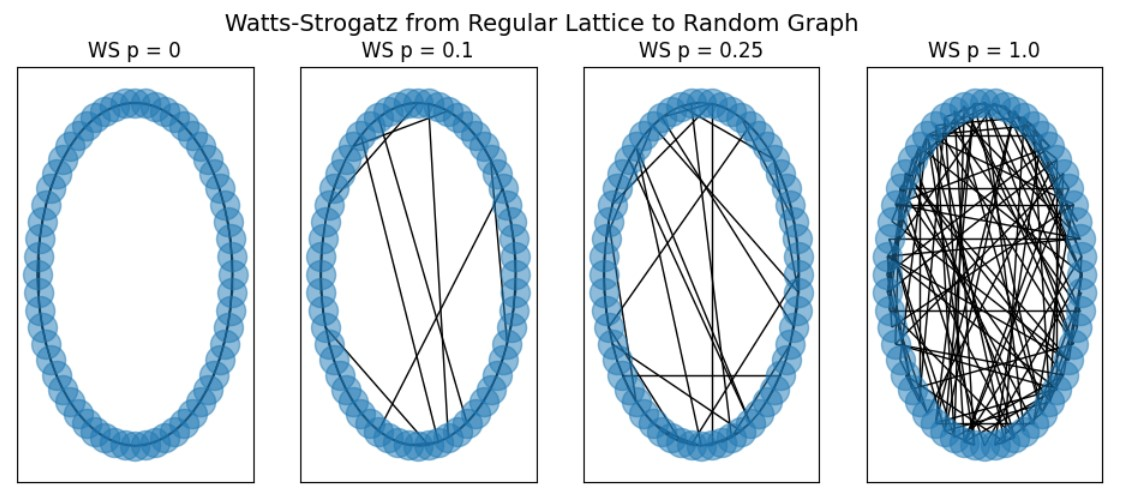
\includegraphics[width=\linewidth]{Figures/order_random.jpg}
	\caption{Watts-Strogatz Graphs with \(n = 60\), \(k = 4\) for different p-values, showing the liminal space between a regular lattice and random graph. \emph{Produced in Python}}
	\label{fig:order_random}
\end{figure*}

\begin{figure*} % Two column figure (notice the starred environment)
	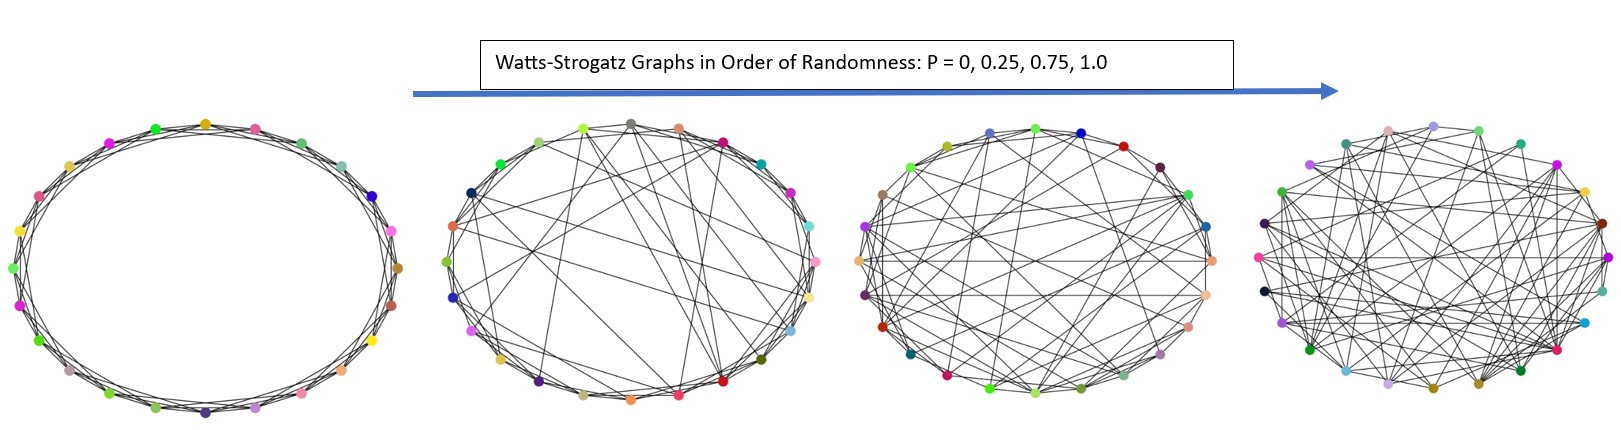
\includegraphics[width=\linewidth]{Figures/order_random_poster.jpg}
	\caption{Watts-Strogatz Graphs with \(n = 24\), \(k = 6\) for increasing p-values, showing the emergence of small-worlds between order and randomness. \emph{Produced in Python}}
	\label{fig:order_random_poster}
\end{figure*}

The implementation was verified ahead of simulations by examining the clustering coefficient and characteristic path-length of the generated graphs. Graphs were generated with size \(n = 1000 \) nodes, lattice neighbours \(k = 10\) and a range of values: 

\begin{align*}
P& = \numberlist{
	0.0001, 0.000125893, 0.000158489, 0.000199526, 0.000251189, 0.000316228, 0.000398107,0.000501187, 0.000630957, 0.000794328, 0.001, 0.001258925, 0.001584893, 0.001995262, 0.002511886, 0.003162278, 0.003981072, 0.005011872, 0.006309573, 0.007943282, 0.01, 0.012589254, 0.015848932, 0.019952623, 0.025118864, 0.031622777, 0.039810717, 0.050118723, 0.063095734, 0.079432823, 0.1, 0.125892541, 0.158489319, 0.199526231, 0.251188643, 
0.316227766, 0.398107171, 0.501187234, 0.630957344, 0.794328235, 1} \label{data:pvalues}
\end{align*} 

The graphs were uniformly assigned a random integer weight for each edge in the range \([0, 100]\). Then, the shortest paths from every node were calculated using Dijkstra's SSSP algorithm and the average of all the shortest path lengths taken for each graph. The clustering coefficient was also computed for each graph generated Figure: \ref{fig:ws_statistics}. \\

\begin{figure} % Single column figure
	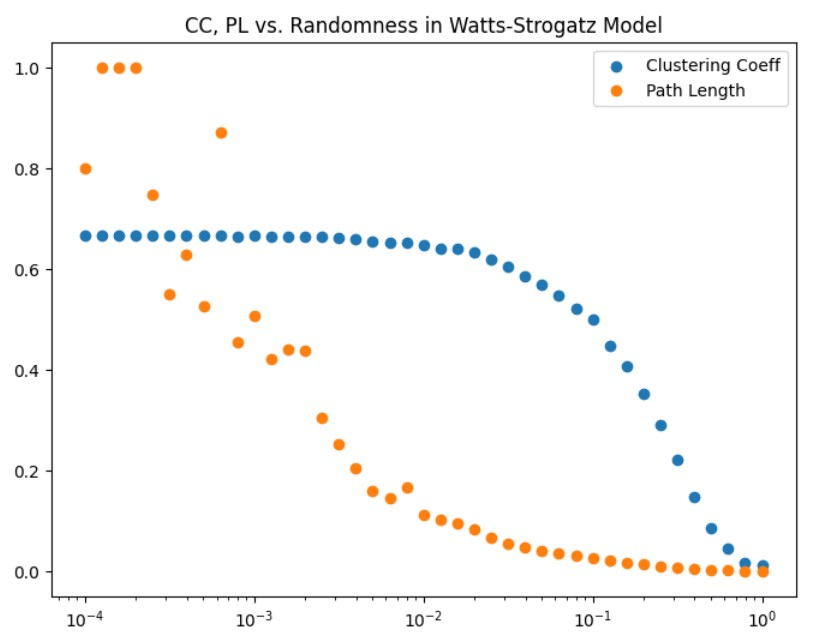
\includegraphics[width=\linewidth]{Figures/ws_statistics_log.jpg}
	\caption{Characteristic Path-Length and Clustering Coefficient for generated WS graphs with a range of P-Values (Logarithmic Scale). \emph{Produced in Python}}
	\label{fig:ws_statistics}
\end{figure}

These results Figure \ref{fig:ws_statistics} follow the original results published by Watts and Strogatz \cite{watts:98}. The clustering coefficient remains high whilst the shortest path length steeply decreased for increase values of \( p \), allowing for small world properties to arise until the network devolves into randomness. 

\subsubsection{Scale-Free Model}

This section will discuss the degree sequence and degree distribution of graphs. The \emph{degree} of a vertex in a graph is the number of edges that it shares with other nodes. In undirected graphs, the \emph{degree} refers to the count of all edges connected to the node. However, in directed graphs, vertices are referred to as having \emph{in-degree} and \emph{out-degree}, referring to the edges directed \emph{in} originating at the neighbour node and edges directed \emph{out} originating at the vertex itself, respectively. The \emph{degree sequence} of a graph is the set of degree values for all vertices, often given in descending order. The \emph{degree distribution} is determined by the number of vertices having each unique degree value in the network. \\

Informally, a network with the Scale Free (SF) property has a very few nodes that are share a high number of connections with other nodes, whilst the majority of nodes have fewer connections. In SF networks, densely connected nodes can act as communication hubs between sparsely connected majority. Formally, an SF network is characterised by it's degree distribution, where the fraction of nodes with degree \(k\) follows a power-law \(k^{-\gamma}\) (Eq. \ref{eq:sf_law}). 

\begin{equation}
	P_{deg}(k) \propto k^{-\gamma}
	\label{eq:sf_law}
\end{equation}

This rule enforces that the number of nodes with degree \(k\) decreases steeply for higher values of \(k\). Across scientific fields it has been claimed that the majority of real-world, both natural and technological, networks are scale free \cite{broido:19}. However, the details of these claim vary; for instance, the requirement for the value of \(\gamma\) varies and it is often only required that the power-law apply for the largest degrees whilst the lower tail of the distribution may devolve to another shape. In any case, the use and study of SF networks is widespread throughout network science including with respect to the study of communication and wireless networks \cite{broido:19}. 

For example, studies of subsets of the World Wide Web (WWW) have identified a SF structure with exponent \(\gamma = 2.1\) \cite{albert:02}; the Internet, actor casting and paper citation have also been identified to have a power-law distribution with \(\gamma = 2.1\), \(\gamma = 2.3\), \(\gamma = 3\), respectively. SF models have been used to study and improve the performance of network types relevant to the DSPRP, for example Internet of Things (IoT) and Wireless Sensor Networks (WSN) \cite{sohn:17}.\\

Barabasi and Albert proposed the random network model to generate graphs with degree distributions that fit the empirically obersved power-law. The Barabasi-Albert (BA) model conceptualises SF networks as evovling from an initial fully-connected topology. New nodes are successively added to the network and are preferentially connected with existing nodes having high degree \cite{albert:99}:

	\begin{enumerate}
		\item Begin with a fully connected topology of a small number \(m_0\) of nodes.
		\item Iteratively until the desired network size is achieved, or for every time step in a simulation of network evolution, add a new node having some value \(m \leq m_{0}\) edges with the existing nodes.
		\item Preferentially draw edges between a new node \(i\) and existing node \(j\) with probability \(P_{ij}\) (Eq. \ref{eq:ba_prob} which depends upon the contribution of the degree of node \(j\), \(k_{j}\), to the sum of degrees:
		\begin{equation*}
			P_{ij}(k_{j}) = \frac{k_{j}}{\sum_{n}k_{n}}
			\label{eq:ba_prob}
		\end{equation*}
		\item From \(t\) time-steps or iterations, emerges a network with \(N = t + m_{0}\) nodes and \(mt\) edges. 
	\end{enumerate}
	
The intended shape of a degree distribution following a power law can be examined by drawing random samples following a power law. Figure \ref{fig:powerlaw_log} depicts the count and fraction of `nodes' having degree \(k\), where rather than generating a network random samples \(r_{i}\) are coerced to a power-law with Eq. \ref{eq:power_law}.

\begin{equation}
	Pl_{i} = ((\Delta^{\gamma + 1} -  \delta^{\gamma + 1}) * r_{i} + \delta^{\gamma + 1})^{(1 / (\gamma + 1))}
	\label{eq:power_law}
\end{equation}

\begin{figure} % Single column figure
	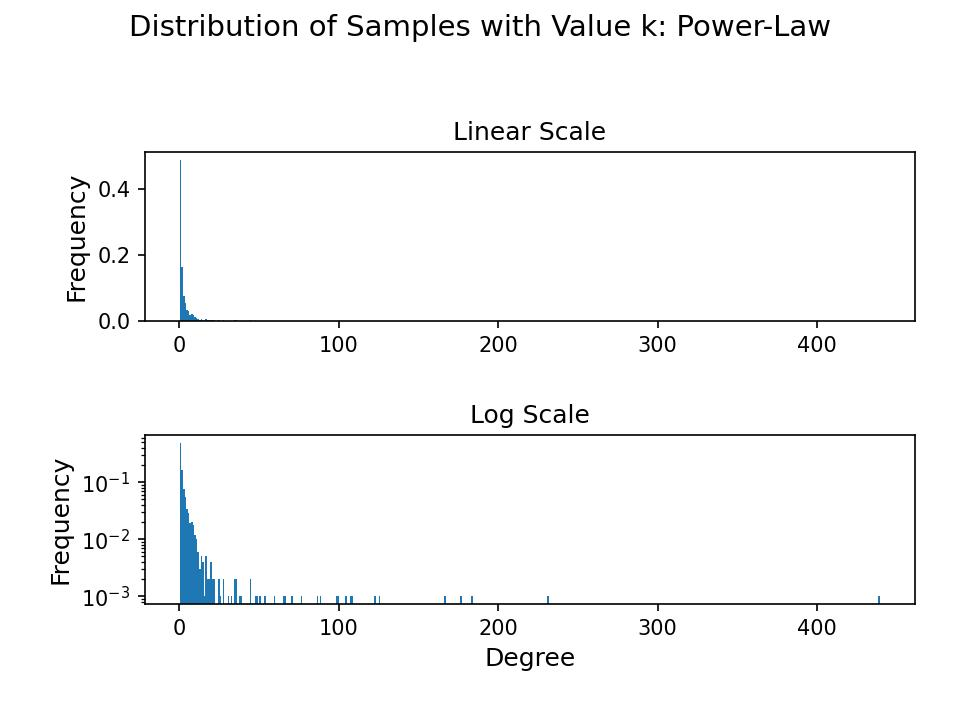
\includegraphics[width=\linewidth]{Figures/ba/power_law_dist.jpg}
	\caption{Distribution of \(1000\) random samples following a power-law produced with Eq. \ref{eq:power_law} for where \(\Delta = 999\), \(\delta = 1\) and \(\gamma = 2\) \emph{Produced in Python}}
	\label{fig:powerlaw_log}
\end{figure}

Where \(\Delta\) refers to the maximum value/degree; \(\delta\) refers to the minimum value/degree; \(\gamma\) refers to the power-law exponent which tends to have a value \(2 \leq \gamma \leq 3\) empirically \cite{albert:02}. The degree distribution of a network can be recognised as following a power-law by plotting it on a log-log scale, wherein the distribution will tend to fall on a descending line which spreads as the degree increases. The samples from Figure \ref{fig:powerlaw_log} are can be seen on a log-log scale in Figure \ref{fig:powerlaw_loglog}. 

\begin{figure} % Single column figure
	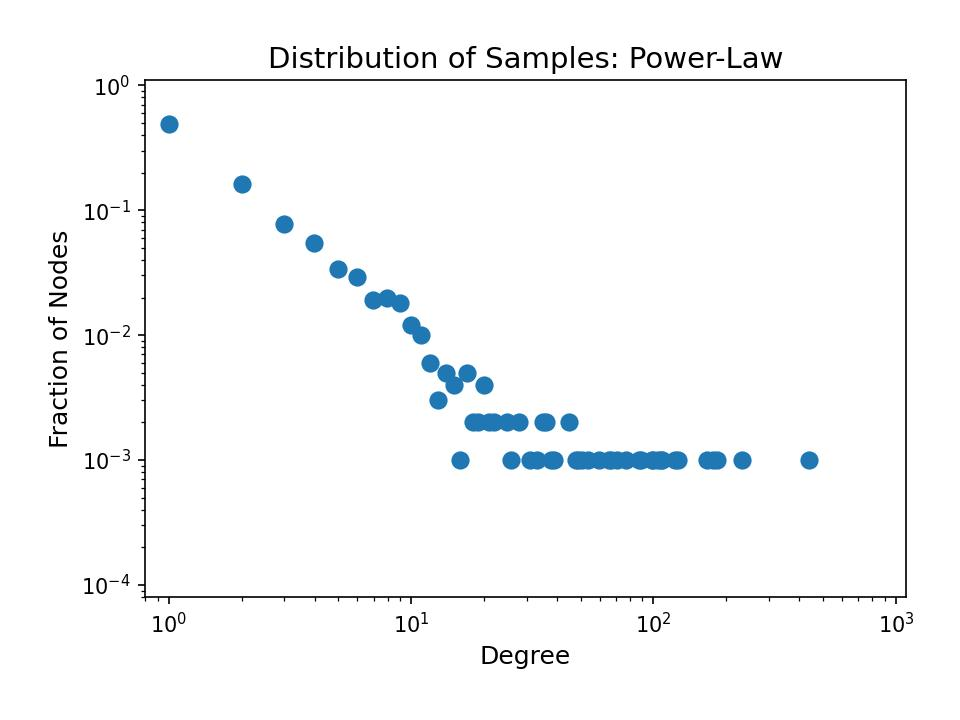
\includegraphics[width=\linewidth]{Figures/ba/power_law_dist_loglog.jpg}
	\caption{Distribution on Log-Log scale of \(1000\) random samples following a power-law produced with Eq. \ref{eq:power_law} for where \(\Delta = 999\), \(\delta = 1\) and \(\gamma = 2\). \emph{Produced in Python}}
	\label{fig:powerlaw_loglog}
\end{figure}

This paper implements the BA model programmatically and generates random networks which can be verified as having scale-free properties. The implementation follows the outline provided by Barabasi \& Albert \cite{albert:99}. For a simple generated network, the preferential structure can be well visualised as in Figure \ref{fig:sf_poster} where a few central nodes have high degree whilst the outer majority have few connections. The degree distribution is also as expected on a linear scale although the power-law is best is best identified on a Log-Log scale. \\

\begin{figure} % Single column figure
	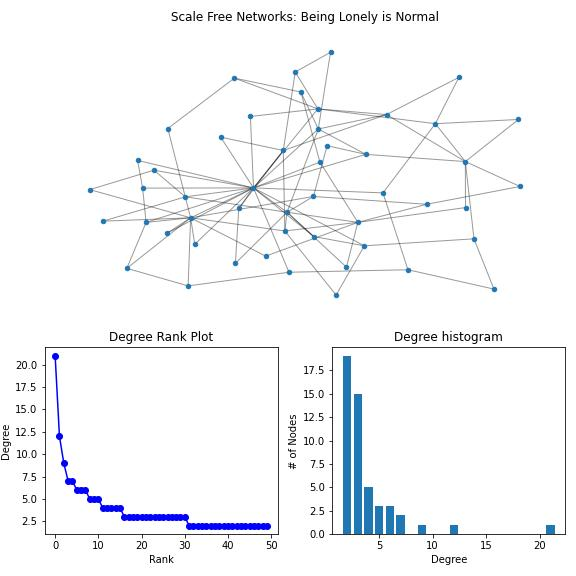
\includegraphics[width=\linewidth]{Figures/ba/sf_poster.jpg}
	\caption{Example Barabasi-Albert SF random network and degree histogram. \emph{Produced in Python}}
	\label{fig:sf_poster}
\end{figure}

Figure \ref{fig:example_sizes} presents three random graphs produced with the BA model of each network size that will be investigated in this paper. By examination of the degree distribution of the generated graphs, the scale-free structure can be verified. For a large \(n = 500\) graph, the degree distribution can be seen as having the expected shape and smooth density estimate (Kernel Density Estimate) in Figure \ref{fig:sf_kde} on a linear scale. The same shape can be seen for the distribution of a larger graph in Figure \ref{fig:dist_large}. When the same distribution is presented on a Log-Log scale in Figure \ref{fig:dist_loglog} it can be seen that the distribution falls along a descending line as is characteristic for power-law networks and compares well with the example given in Figure \ref{fig:powerlaw_loglog}. 

\begin{figure*} % Single column figure
	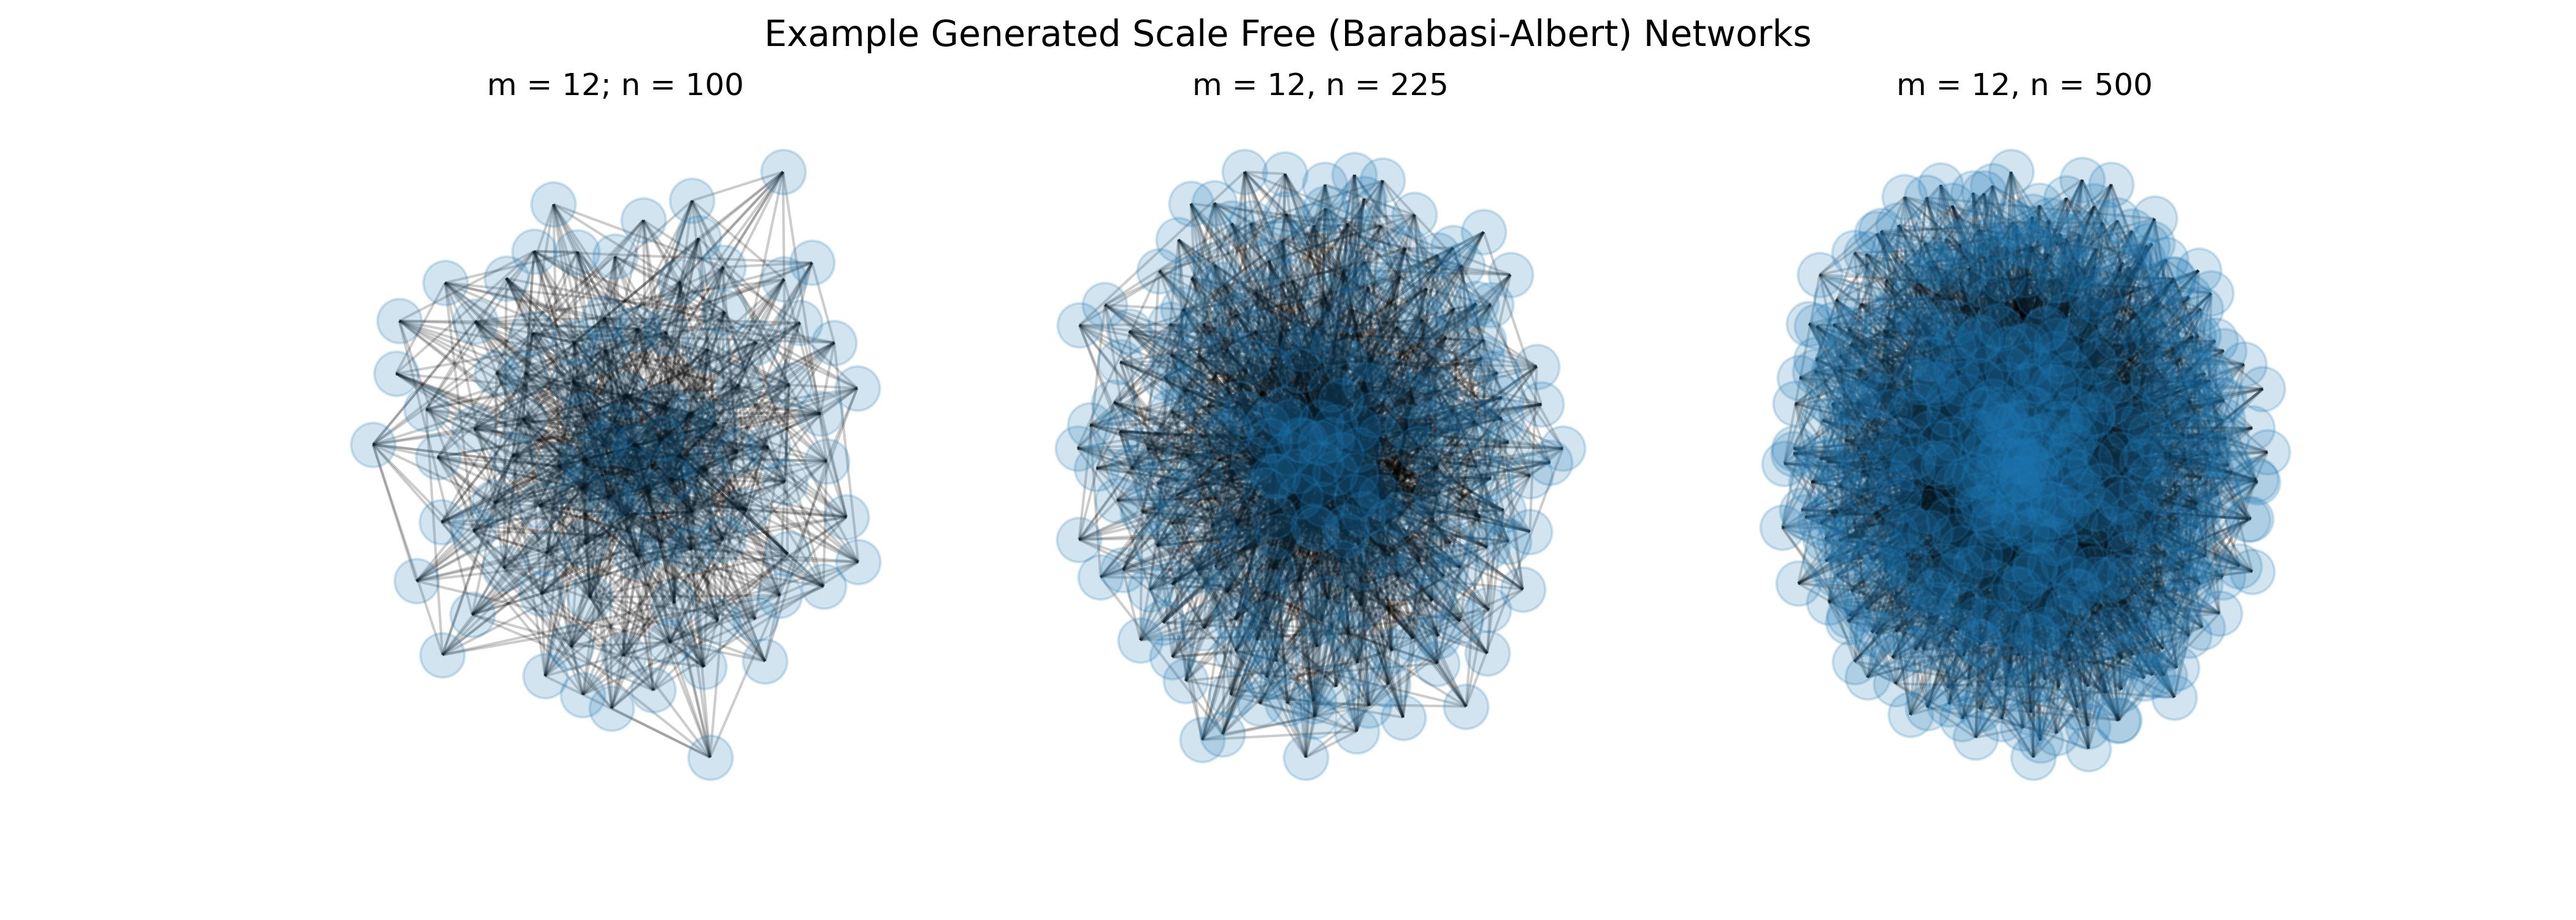
\includegraphics[width=\linewidth]{Figures/ba/example_sizes.jpg}
	\caption{Example Barabasi-Albert SF random networks of simulation sizes \(n = 100, 225, 500\). \emph{Produced in Python}}
	\label{fig:example_sizes}
\end{figure*}

\begin{figure}[H] % Single column figure
	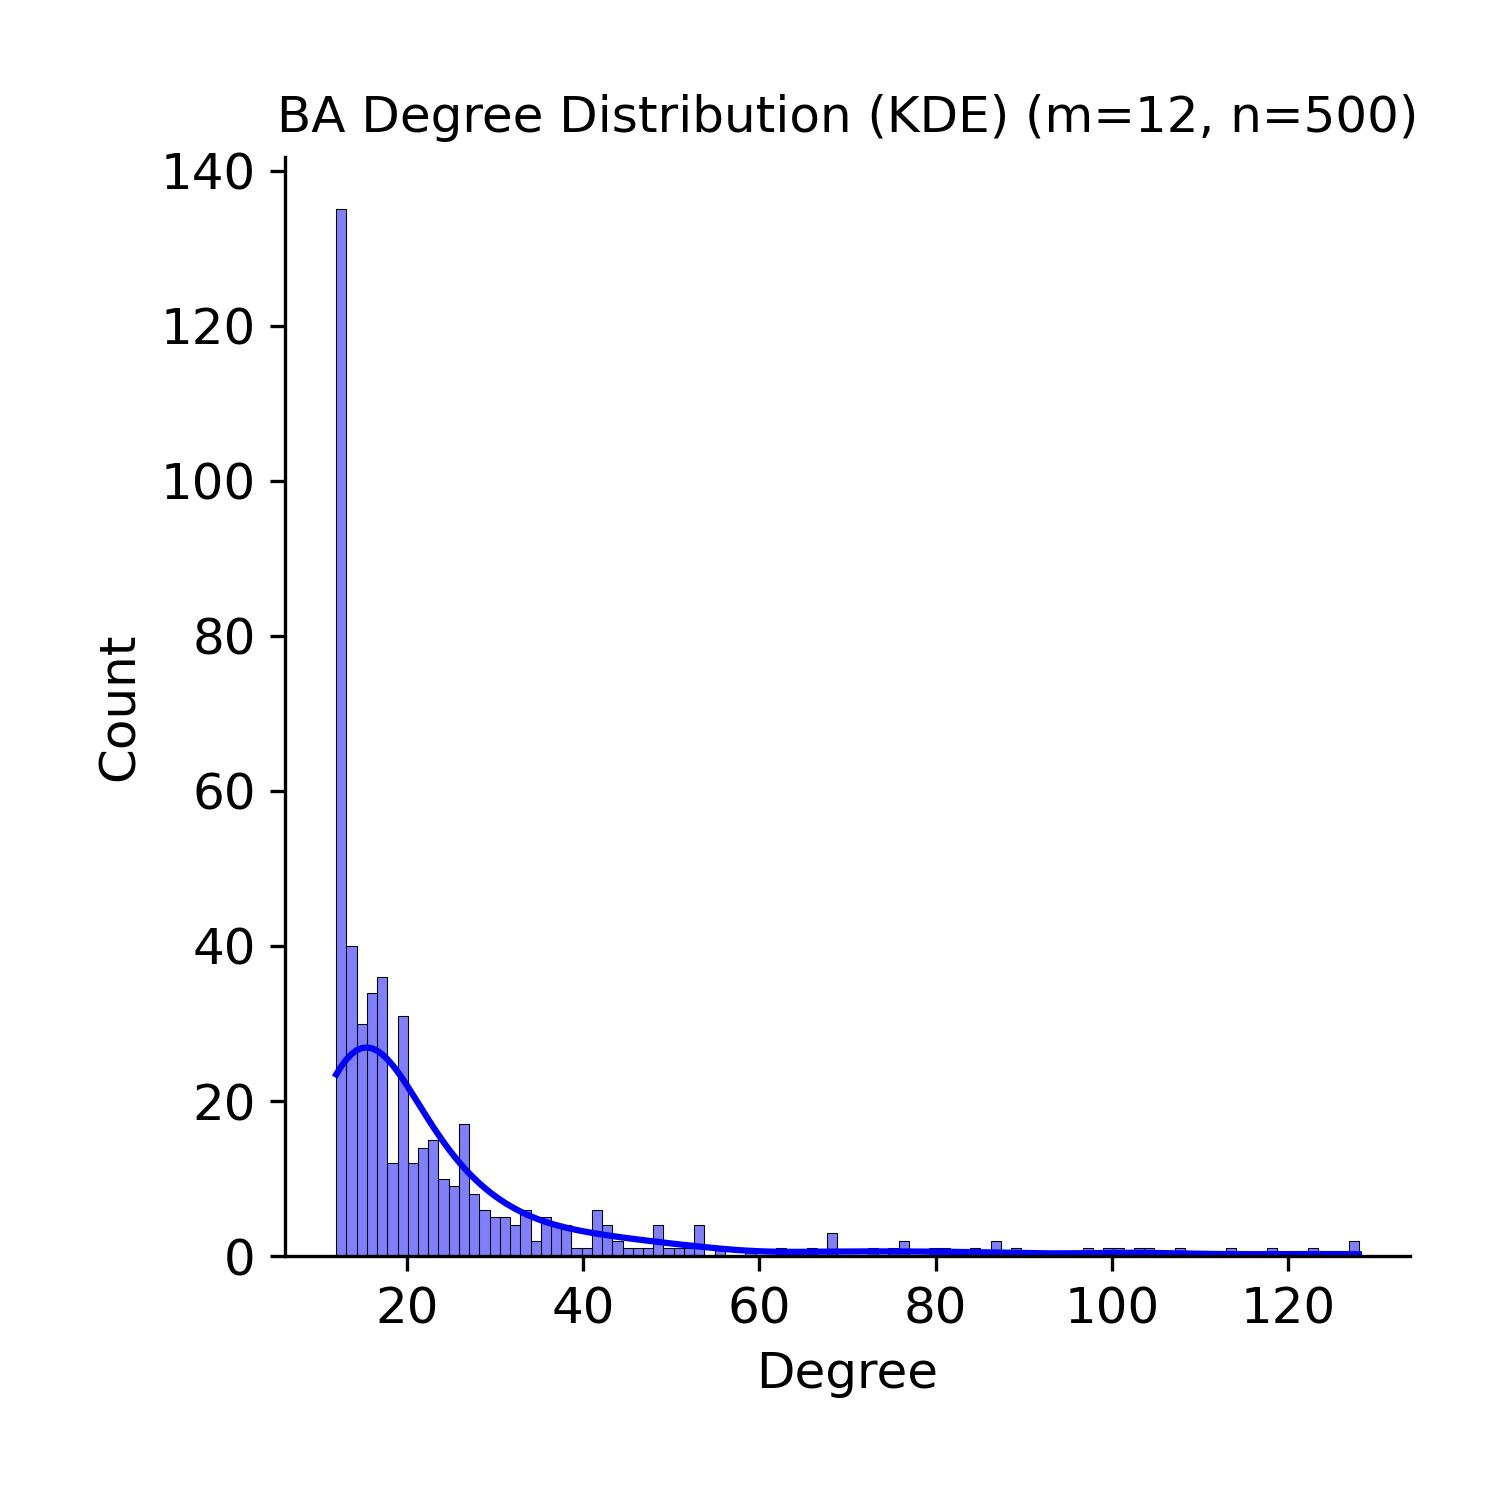
\includegraphics[width=\linewidth]{Figures/ba/degree_density_500.jpg}
	\caption{Degree distribution and Kernel Density Estimate (smooth line) of BA network \(m=12, n=500\) following a power-law.  \emph{Produced in Python}}
	\label{fig:sf_kde}
\end{figure}

\begin{figure}[H] % Single column figure
	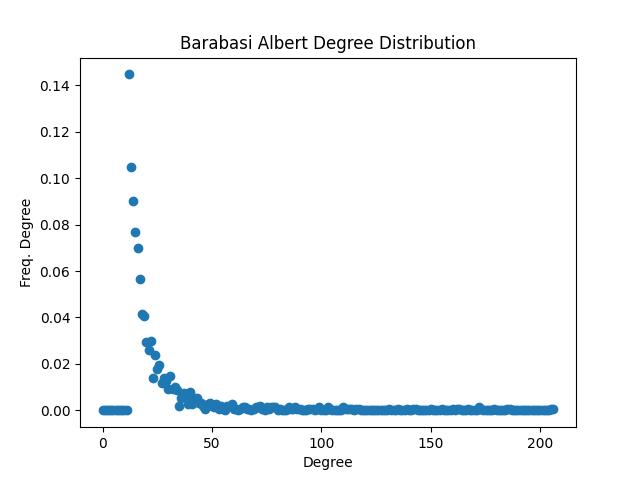
\includegraphics[width=\linewidth]{Figures/ba/ghetto_degree_dist.jpg}
	\caption{Degree distribution of the BA graph \(m = 12, n = 1500\) from Figure \ref{fig:dist_loglog} a scatter plot in linear scale. \emph{Produced in Python}}
	\label{fig:dist_large}
\end{figure}

\begin{figure}[H] % Single column figure
	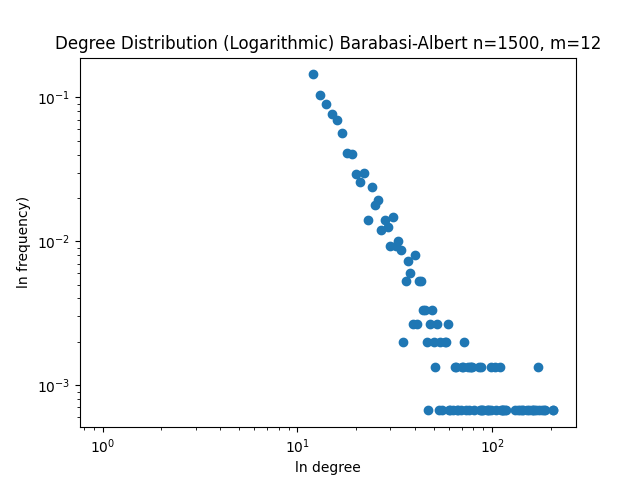
\includegraphics[width=\linewidth]{Figures/ba/degree_dist_log.png}
	\caption{Degree distribution in Log-Log scale of BA network \(m=12, n=1500\) illustrating the characteristic shape where samples follow a power-law.  \emph{Produced in Python}}
	\label{fig:dist_loglog}
\end{figure}

% Add additional plots for prosperity 

\begin{figure}[H] % Single column figure
	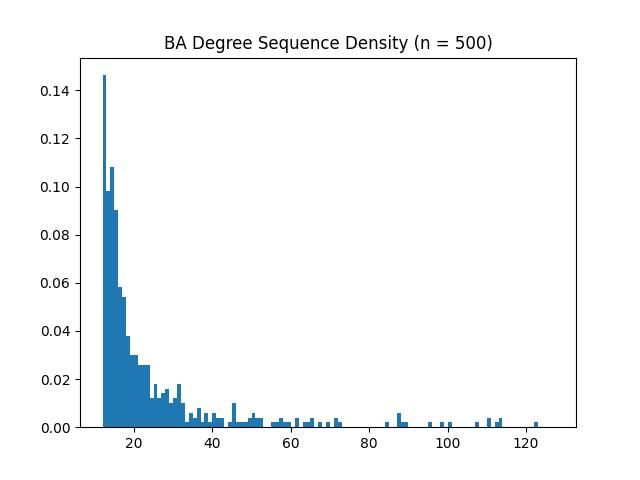
\includegraphics[width=\linewidth]{Figures/ba/degree_dist_density.jpg}
	\caption{Degree distribution density plot in linear scale of a generated BA network \(m=4, n=500\). \emph{Produced in Python}}
	\label{fig:sf_degree_density}
\end{figure}

\begin{figure}[H] % Single column figure
	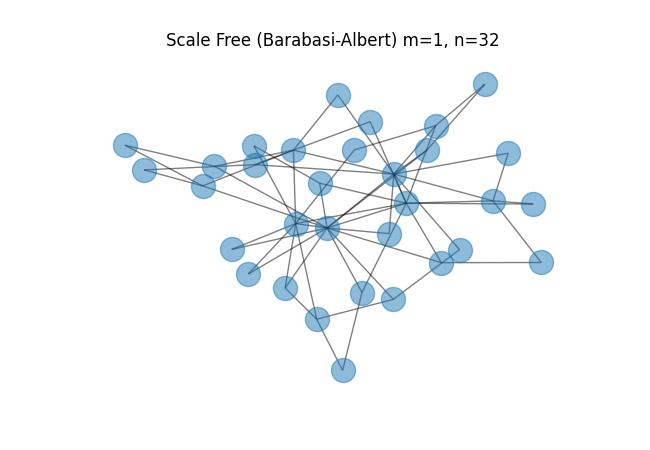
\includegraphics[width=\linewidth]{Figures/ba/example_m1.jpg}
	\caption{Example generated BA graph with minimum starting graph \(m = 1\).  \emph{Produced in Python}}
	\label{fig:sf_example_m1}
\end{figure}

\begin{figure}[H] % Single column figure
	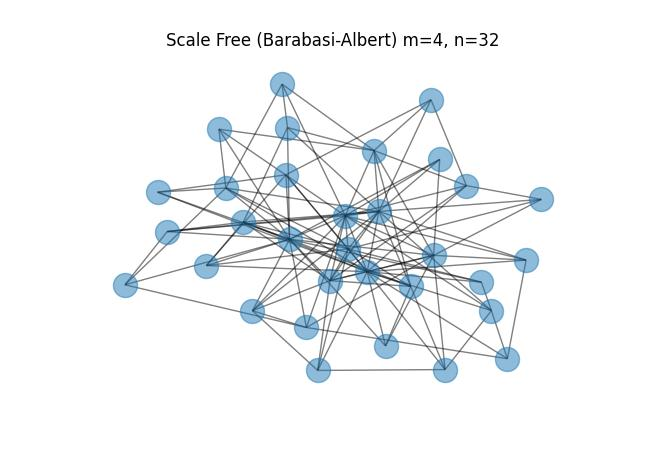
\includegraphics[width=\linewidth]{Figures/ba/example_small.jpg}
	\caption{Example generated BA graph with small starting graph \(m = 4\). \emph{Produced in Python}}
	\label{fig:sf_example_small}
\end{figure}

\subsubsection{Log-Normal Model} 
Though real-world networks are often claimed to be scale-free and many studies have supported sale-free properties to be widespread in a variety of domains both natural and technological \cite{broido:19}, the ubiquity of scale-free networks is contended in the literature. Broido \& Clauset note that the statistical methods used for performing network analysis vary as do the precise definitions of scale-free networks themselves, possibly leading to misdiagnosis of scale-free properties \cite{broido:19}. \\

Broido \& Clauset find in a rigorous analysis with improved analytical methods and a hierarchy of increasingly strict definitions of `scale-free' properties, that of ~1000 large networks, including technological and information networks, strongly scale-free networks having exponent \(2 \leq \gamma \leq 3 \) and where the power-law is obeyed throughout the distribution are empirically rare, whilst most networks studied are at best weakly scale-free where a power-law is obeyed within the upper-tail (highest degrees) of the distribution \cite{broido:19}. Broido \& Clauset find that for the majority of networks studied, at least 50\% of the network structure fits better to an alternative distribution. \\

Smith \cite{smith:21} offers an alternative model that can represent the commonly observed shared characteristics of complex networks that may otherwise be considred scale-free. Smith presents a model for complex networks that out performs ``popular power-law fitness explanations'' across 110 networks. The degree distribution of the modelled networks obeys a power-law at low densities and a log-normal distribution at larger densities. Overall, Smith concludes that log-normal distributions are more common and a better fit to most complex networks than a power-law. \\

Informally, The log-normal distribution is a continuous probability distribution of the exponential function of a normally distributed random variable. Inversely, the log-normal distribution is the probability distribution of a random variable the logarithm of which is normally distributed. Formally, a positive random variable \(X\) is log-normally distributed \(X \propto Lognormal(\mu_{x}, \sigma_{x}^{2}\) if the natural logarithm of \(X\) is normally distributed \(ln(X) \propto \mathcal{N}(\mu, \sigma^{2}\). Figure \ref{} visualises the distribution of \( 1000 \) samples of a log-normally distributed random variable  with \( \mu = 0, \sigma = 1 \) and probability density, given by Eq. \ref{eq:lognormal_pdf}. 

\begin{equation}
	p(x) = \frac{1}{\sigma{x}\sqrt{2\pi}}e^{-\frac{(ln(x) - \mu)^{2}}{2\sigma^{2}}}
	\label{eq:lognormal_pdf}
\end{equation}

\begin{figure}[H] % Single column figure
	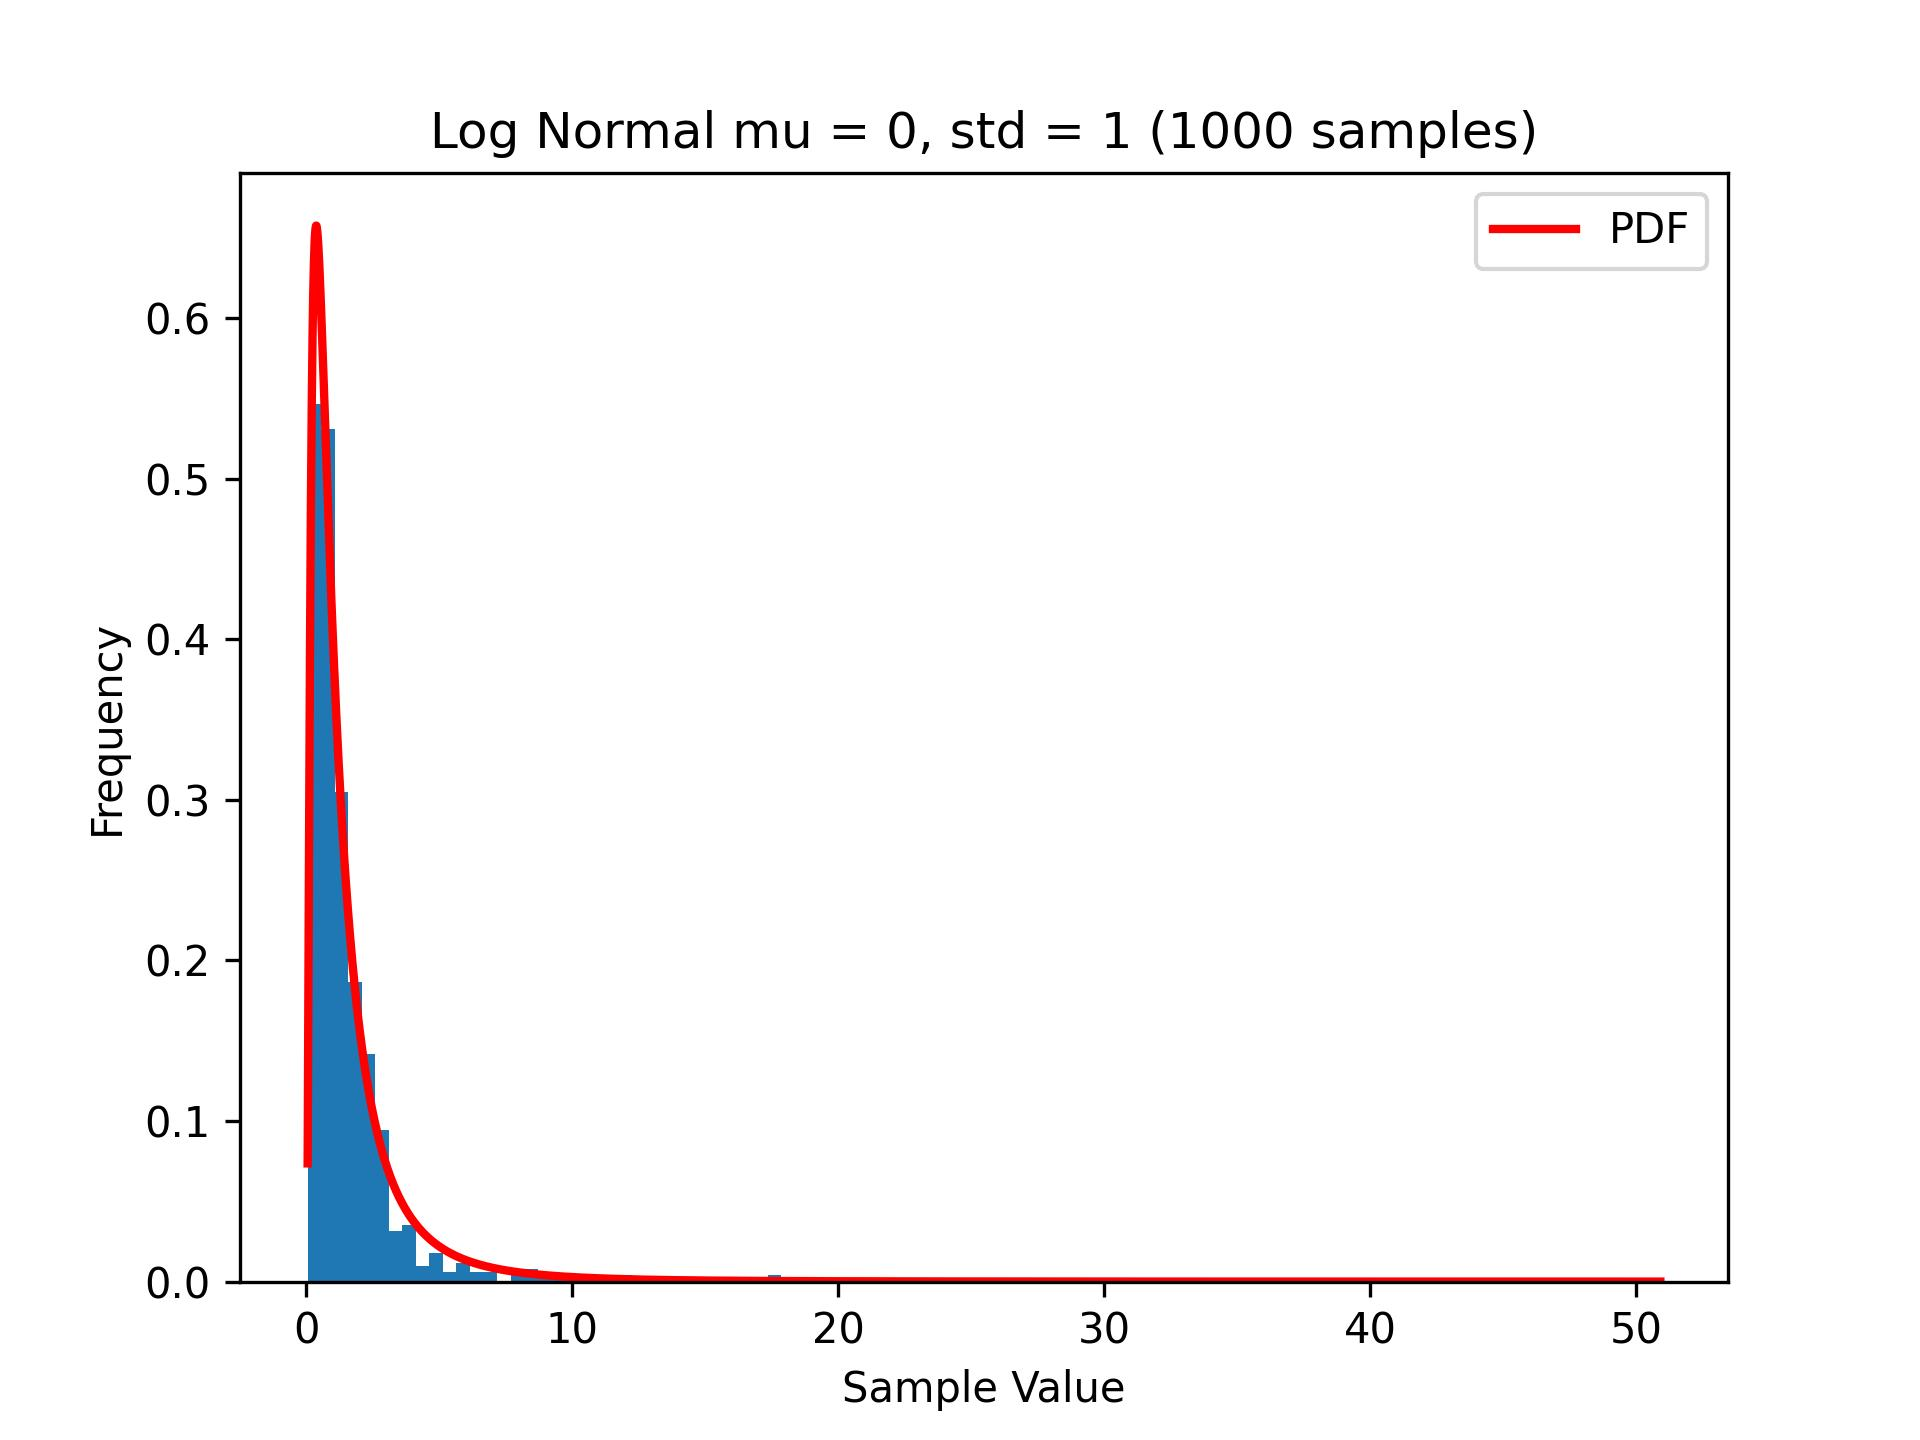
\includegraphics[width=\linewidth]{Figures/ln/lognormal_dist.jpg}
	\caption{Distribution/Probability Density Function (PDF) of a log-normal random variable. \emph{Produced in Python}}
	\label{fig:lognormal_dist}
\end{figure}

Considering the trends in the literature with respect to accurate modelling of complex networks, this paper proposes to model random networks having Log-Normal degree distribution for investigation in simulations. Smith presents a network model with two core components: (1) A ``surface factor'' assigned to each network node indicating it's independent, individual tendency to form connections; (2) A ``depth factor'' which represents the dyadic propensity of nodes to form connections, and is inversely proportional to their distance in Euclidean space. \\ 

Let \(V = {1, ..., n} \) be the set of nodes in a network. Each node is assigned a surface value  \( s_{i} \) that represents its individual tendency to form connections. This can be conceptualised as the size of the node, wherein larger nodes are more likely to form connections. Smith draws a conceptual parallel between the surface factor and empirically observed latent variables in network formation, such as the individual traits of extroversion and charisma which may effect a persons likelihood to form relationships in a human social network. \\

The depth factor represents dyadic information between two nodes that formalises the homophily principle that contact between similar network entities is more frequent than disimilar entities. Smith conceptualises latent spaces as encoding similarities between nodes, and formalises this as \(q\)-dimensional Euclidean space in which nodes are assigned coordinates. These coordinates may be considred as \(q\) latent variables \(x_{1}, x_{2}, ..., x_{q}\). Then, the similarity of two nodes can be given by some inverse distance function: \(d_{ij} = f(x_{1}(i), x_{1}(j), x_{2}(i), x_{2}(j), ..., x_{q}(i), x_{q}(j)) \). \\

This paper proposes to use the simplest realisation of Smith's concept: Nodes are assigned a position in Euclidean space uniformly in the interval \([0, 1]\), then the depth factor is calculated as the inverse of the straight-line distance pairs of nodes. This is such that, nodes that are close together are regarded as being similar, and will have a greater propensity of forming connections with one another and the depth factor can be given as in Eq. \ref{eq:depth_factor}. Though it is likely latent variables will have different distributive properties with respect to real-world networks, Smith \cite{smith:21} that uniform placement fits well to a variety of complex networks. \\

\begin{equation}
	d_{ij} = exp(-\sqrt{\sum_{k=1}^{q}(x_{ik} - x_{jk})^{2}})
	\label{eq:depth_factor}
\end{equation}

With respect to the surface values of nodes, Smith considers whether the individual tendencies are multiplicative or additive between pairs of nodes. The surface factor between two nodes is best computed as the addition of their surface values, as this relationship allows the sum of surface factors from a node \(s_{i}\) to all other nodes to scale linearly with \(s_{i}\). Hence, the surface factor is given in Eq. \ref{eq:surface_factor}.

\begin{equation}
	S_{ij} = (s_{i} + s_{j}) 
	\label{eq:surface_factor}
\end{equation}

Then, the probability of a connection being established is proportional to both the similarity of the nodes given by the depth factor and the combined individual tendency to form connections (Eq. \ref{eq:ln_prob}). Smith suggests that the edge weights can be taken as the product of the depth factor with the surface factor, however this paper takes the inverse for the weights such that disimillar/distant nodes will tend to be more expensive to traverse (Eq. \ref{eq:ln_weight}). 

\begin{equation}
	p_{ij} \propto d_{ij}(s_{i} + s_{j})
	\label{eq:ln_prob}
\end{equation}

\begin{equation}
	w_{ij} = (d_{ij}(s_{i} + s_{j}))^{-1}
	\label{eq:ln_weight}
\end{equation}

For this paper, the below procedure is followed to generate log-normally distributed graphs from Smith's surface-depth model in Python:
	\begin{enumerate}
  		\item \(n\) nodes are uniformly assinged coordinates on a 2D Euclidean plane. 
  		\item \(n\) samples are drawn from a log-normal distribution \(LN(\mu, \sigma)\) for \(\mu = 0.0\) and \(\sigma = 1.0\) and assigned to each node by array index. 
  		\item The straight-line distance \(d_{ij}\) between all pairs of nodes \((i, j)\) is calculated from the node coordinates.
  		\item The surface factor of each pair of nodes \((i, j)\) is taken as the sum of the individual surfaces \(S_{ij} = s_{i} + s_{j}\).
  		\item The link probability is taken as proportional to the product of the depth and surface factors for each pair of nodes \(Pr_{link} \propto d_{ij}(s_{i} + s_{j})\). 
  		\item Links are selected to be formed between pairs of nodes proportional to their link probability with Stochastic Universal Sampling (SUS) up to the desired number of edges \(M\) 
  		\item Edge weights \(w_{ij}\) are assigned with Eq. \ref{eq:ln_weight}. 
  		\subitem This process is repeated from scratch until a connected topology is formed 
	\end{enumerate}
	
Considering that the other network models used in this project do not provide a formula for weighting edges, the edge weights of all networks including log-normal are set to a random integer in the range \([1, 100]\) for DSPRP simulations. \\

The simulations in this paper assume a connected topology for each graph examined, hence the generation process must be repeated until a connected topology is formed. The implementation of this mathematics can be verified by plotting the degree distribution of generated networks.  Figure \ref{fig:ln_degree_dist} shows the degree distribution of a generated graph for comparison with the expected distirbution presented in Figure \ref{fig:lognormal_dist}. Figure \ref{fig:ln_example_sizes} gives examples of three networks of sizes \(100, 225, 500\) ndoes generated with the above procedure. 

\begin{figure}[H] % Single column figure
	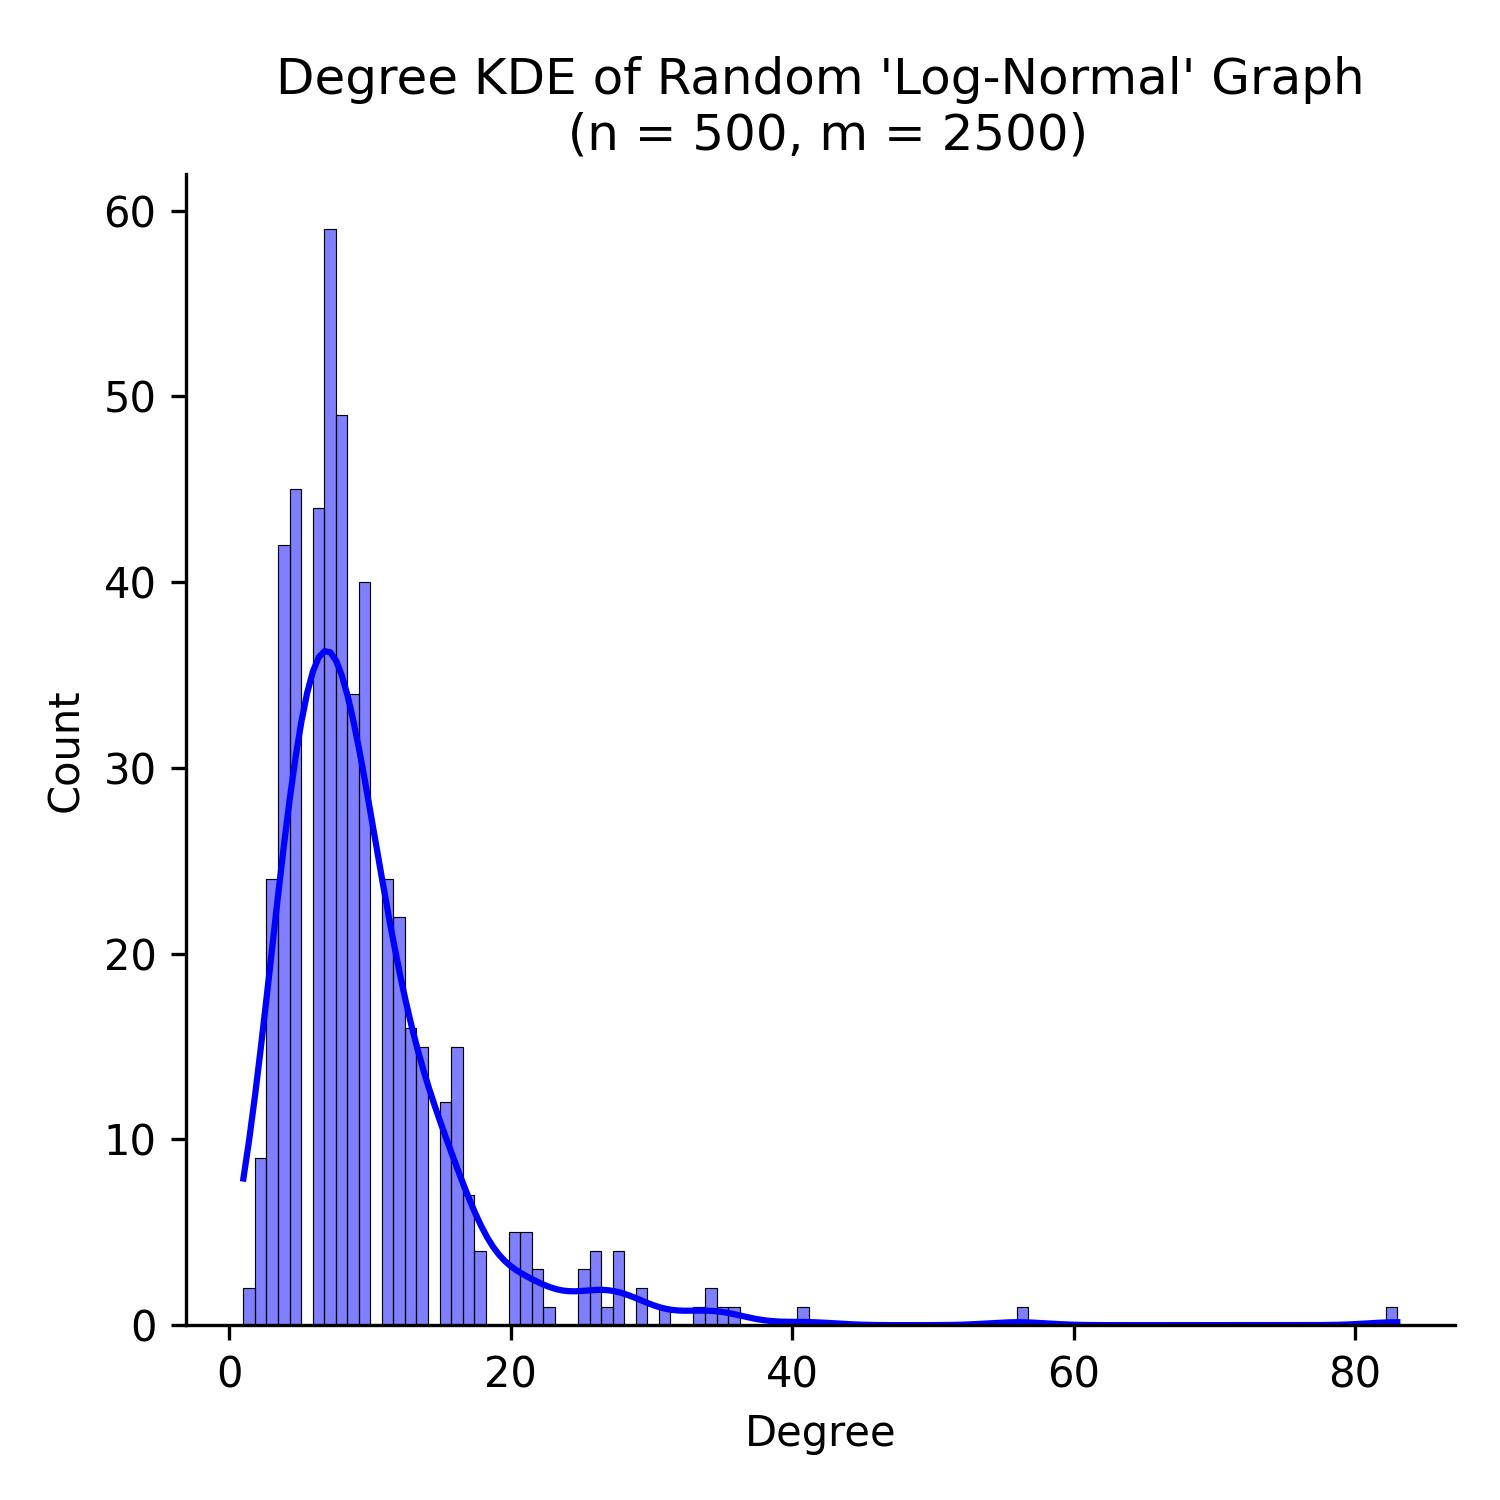
\includegraphics[width=\linewidth]{Figures/ln/ln_degree_dist.jpg}
	\caption{Degree Distribution and Kernel Density Estimation (smooth line) a network generated with the procedure proposed by Smith \cite{smith:21}. \emph{Produced in Python}}
	\label{fig:ln_degree_dist}
\end{figure}

\begin{figure*}
	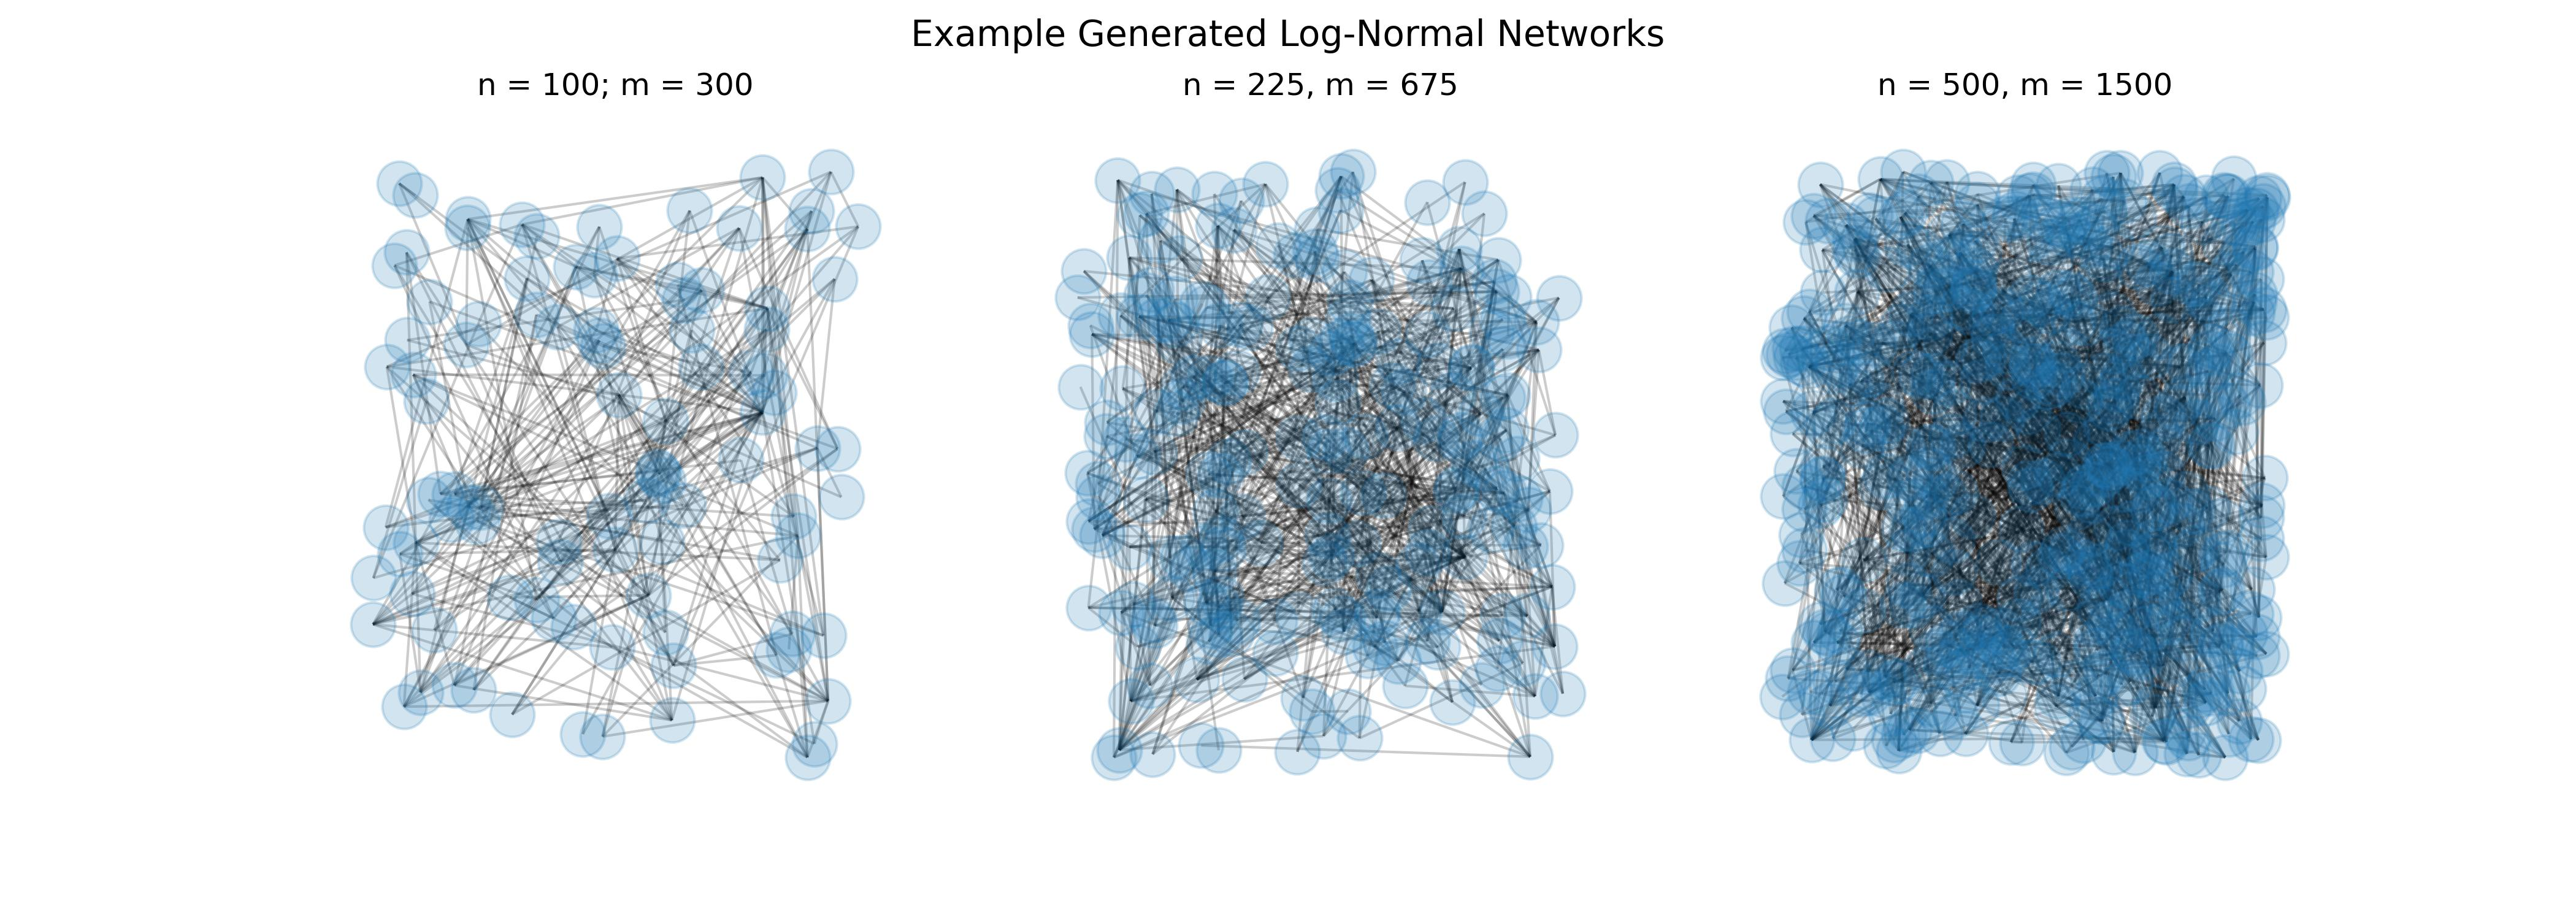
\includegraphics[width=\linewidth]{Figures/ln/example_sizes.jpg}
	\caption{Networks of sizes \(n = 100, 225, 500\) generated with the procedure proposed by Smith \cite{smith:21}\emph{Produced in Python}}
	\label{fig:ln_example_sizes}
\end{figure*}

Considering that it is not evident that any programmatic implementation of Smith's model \cite{smith:21} or another generative algorithm for producing random graph models with log-normal degree distribution - excluding generic algorithms for creating a network from a given degree sequence which may be log-normal - is in the public domain, the Python 3.9 implementation for the model is provded here. 

\lstset{
breaklines  = true,
breakatwhitespace   = false,
prebreak= \space,
postbreak   = \space,
language = Python
}

\lstinputlisting[language=Python]{./Listings/log_normal.py}

\subsection{Stochastic Topological Dynamics}

Yang \& Wang propose to simulate topological dynamics in a MANET model by effecting a change at regular intervals given by parameter \(R\), where for each change \(M\) nodes are activated or deactivated dependent upon their existing state. This simulation method is appropriate to represent the sleep-wake cycle of nodes observed in a variety of wireless networks, where node activity may be subejct to conditions such as limited battery life, changing geographical location and wireless connectivity issues \cite{yang:10}. \\

This paper proposes that a more broadly representative and realistic simulation can be achieved by subjecting each network component to its own independent probability of undergoing a change. This is such that, where the probability of a change is the same for each component, the frequency and severity of changes are stochastic as opposed to fixed by Yang \& Wang's \(M, R\) parameters and can be regulated by the single probability paramter. \\

Furthermore, this paper proposes to model topological dynamics effecting each separate aspect of the network: The node/vertex set \(V_{0}\); the edge set \(E_{0}\) and edge weight's, conceptualised in this paper as belonging to the set \(W_{0}\). In real-world dynamic networks, any aspect of the network structure may be subject to change and may affect the shortest routing paths. \\ 

This paper also investigates by how much each model effects the shortest path routes and lengths across the network, for different probabilities. Does the DSPRP require a dynamic solution? Network changes may not neccessarily effect any or all of the shortest paths in the network. The DSPRP benefits from being treated as a dynamic optimisation problem in the case where the shortest paths are frequently affected, such that deterministic calculation becomes intractable. For what probability of a change do such conditions arise? \\

\subsection{Weight Set Dynamics}

The first method investigated for simulating dynamic edge-weights is as follows: For each edge in the network at each time step, the weight is multiplied with some value \(m \sim \mathcal{N}(\mu = 1, \sigma = 0.25)\) drawn from a normal distribution with mean of one and standard deviation of a quater, bounded in the interval \([x, y], x = 0.25, y = 1.75\) to give a change of no greater than \(\frac{3}{4}\) the existing value, with probability \(Pr_{dyn}\). \\

\begin{equation}
	w_{ij}^{t+1} = w_{ij}^{t} \times m
	\label{eq:weight_mult}
\end{equation}

The multiplicative relationship between \(m\) and \(w_{ij}\) allows for proportionally small changes to the weights. Whereas it is not clear what \(\mu, \sigma\) would be used in an additive model. In concept, the coefficient \(m\) may be drawn from any distribution. Placing a normal distribution about mean of 1 with a small standard deviation is intended to encourage small changes with occasional outliers. This model may simulate, for example, a wireless network where the geographical separation of nodes changes resulting in greater/lesser transmission times. Such changes observed in a real-world network will likely obey some well known distribution, which could then be used with this method for simulations. \\

The second method proposed is arguably the simplest: In this model, the edges \(e: (i, j)\) in the graph are iterated, and for each edge the associated weight \(w_{ij})\) is assigned a new random value in the range \([wmin, wmax]\) with probability \(Pr_{dyn}\). By default in this project \(wmin = 1\) and \(wmax = 100\).  \\

\subsubsection{Simulations}

The first set of simulations for effective parameters examines the number of shortest paths changed at each time step in terms of the order of nodes traversed in the path. For each simulation, a new random WS graph is generated. 

\textbf{Simulation 1:} (Figure \ref{fig:ewd_ex1} For a probability of \(Pr_{dyn} = 1\) to update each edge weight, simulations are run for \(ts = 100\) time-steps with a range of standard-deviations: \(0.01, 0.05, 0.1, 0.2\). The total number of shortest paths changed from the previous time-step are calculated with Djikstra's SSSP. Only changes is the nodes/node-order are considered. 

\begin{figure}[H]
	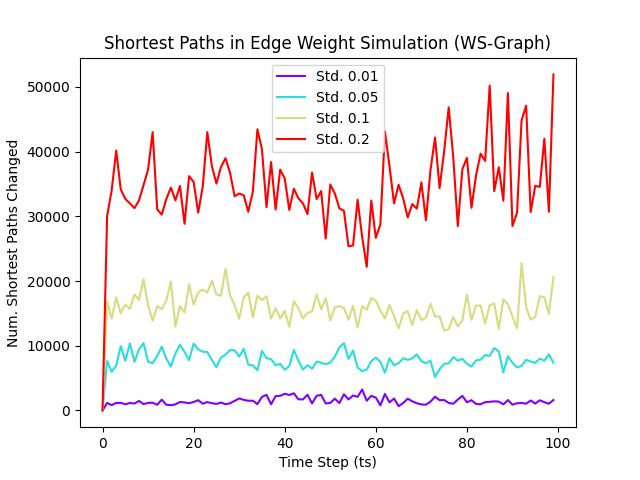
\includegraphics[width=\linewidth]{Figures/ewd/ew1_paths_std.jpg}
	\caption{Number of shortest paths changed for WS graph with Edge Weight Dynamics and a range of standard deviations. (\(Pr_{dyn} = 1\)). \emph{Produced in Python}}
	\label{fig:ewd_ex1}
\end{figure}

\textbf{Simulation 2:} (Figure \ref{fig:ewd_ex2}) For a standard deviation of \(\sigma = 0.2\) a range of probability parameters \(Pr_{dyn} = 0.05, -.25, 0.5, 0.75\) are investigated. For \(ts = 100\) time steps, the number of shortest paths changed from the previous time step are calculated.

\begin{figure}[H]
	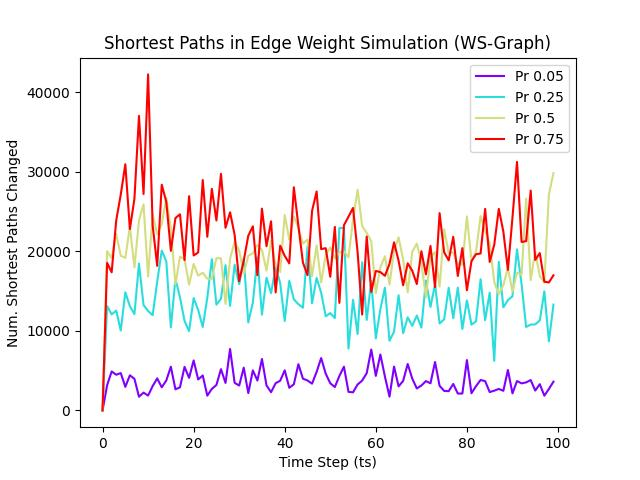
\includegraphics[width=\linewidth]{Figures/ewd/ew1_paths_prob.jpg}
	\caption{Number of shortest paths changed for WS graph with Edge Weight Dynamics, and a range of probability parameters. (\(\sigma = 0.2\)). \emph{Produced in Python}}
	\label{fig:ewd_ex2}
\end{figure}

The second set of simulations for effective parameters aims to examine \emph{by how much} the effected shortest paths change. This is achieved by calculated the average shortest pathlength (characteristic pathlength) at each time step. \\

\textbf{Simulation 3:} (Figrue \ref{fig:ewd_ex3}) For a probability of \(Pr_{dyn} = 1\) to update each edge weight, simulations are run for \(ts = 100\) time-steps with a range of standard-deviations: \(0.05, 0.1, 0.2, 0.3\). The average path length was calculated at each time step. \\

\begin{figure}[H]
	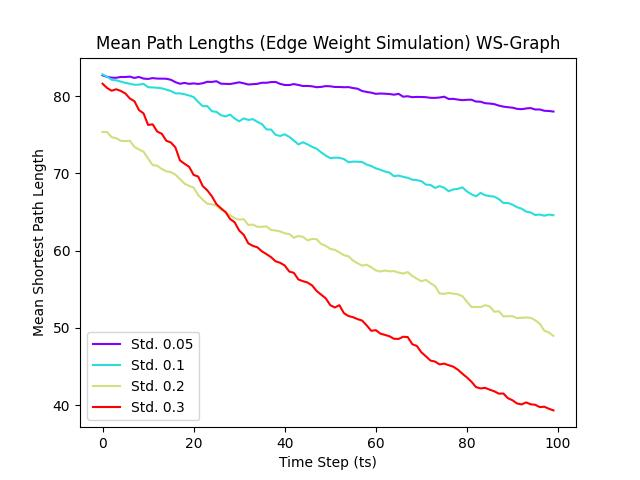
\includegraphics[width=\linewidth]{Figures/ewd/ew1_length_std.jpg}
	\caption{Average shortest path length for \(ts = 100\) time-steps and a range of \(\sigma\). WS Graphs. Edge weight Dynamics. \(Pr_{dyn} = 1\). \emph{Produced in Python}}
	\label{fig:ewd_ex3}
\end{figure}

\textbf{Simulation 4:} (Figure \ref{fig:ewd_ex4}) For \(sigma = 0.1\) and a range of probability parameters \(Pr_{dyn} = 0.05, 0.25, 0.5, 0.75\), the average path length was calculated at \(ts = 100\) time steps. \\

\begin{figure}[H]
	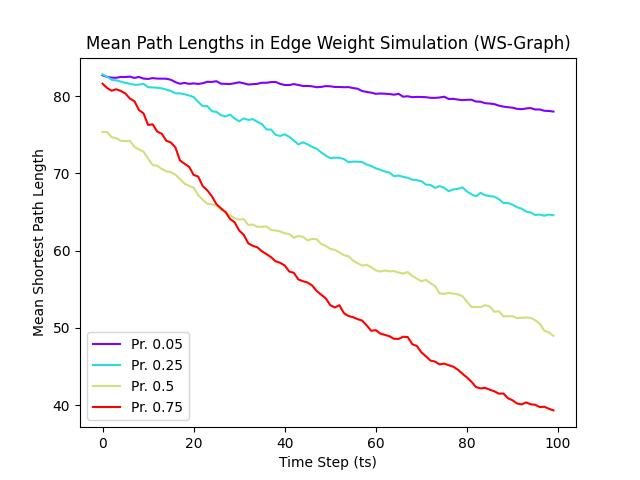
\includegraphics[width=\linewidth]{Figures/ewd/ew1_length_prob.jpg}
	\caption{Average shortest path length for \(ts = 100\) time-steps and a range of \(Pr_{dyn}\). \(\sigma = 0.1\) WS Graphs. Edge weight Dynamics. \emph{Produced in Python}}
	\label{fig:ewd_ex4}
\end{figure}

In summary, results show that a significant number of shortest paths are changed at each time step and that the mean number of paths changed increases in proportion to both the frequency, given by \(Pr_{dyn}\), and the severity of the change given by \(\sigma\). \\

Interestingly, calculation of the average path length shows that for this dynamic model the average shortest pathlength tends towards zero. This is unrealistic and would cause DSPRP simulations to provide biased results and quickly devolve. \\

Hence, the second model is proposed in which effected edge weights are simply assigned a new uniform random value in the given interval. Figure \ref{fig:ewd_ex5} examines the effect of different values of \(Pr_{dyn}\) on the number of shortest paths changed in each iteration (Simulation 5). Figure \ref{fig:ewd_ex6} evaluated the average path length for the same values of \(Pr_{dyn}\) and verifies that the path lengths in the network do not tend towards zero, whilst showing more variance with higher \(Pr_{dyn}\) values. \\

\begin{figure}[H]
	\includegraphics[width=\linewidth]{Figures/ewd/ew2_ex1_paths.jpg}
	\caption{Number of shortest paths changed for \(ts = 100\) time-steps and a range of \(Pr_{dyn}\) WS Graphs. Edge weight Dynamics. \emph{Produced in Python}}
	\label{fig:ewd_ex5}
\end{figure}

\begin{figure}[H]
	\includegraphics[width=\linewidth]{Figures/ewd/ew2_ex2_lengths.jpg}
	\caption{Average shortest path length for \(ts = 100\) time-steps and a range of \(Pr_{dyn}\). WS Graphs. Edge weight Dynamics. \emph{Produced in Python}}
	\label{fig:ewd_ex6}
\end{figure}

\subsection{Edge Set Dynamics}
Dynamics of the edge set are modelled as follows: For each edge \(e: (i, j)\) in \(E_{i}\), replace the edge with a new edge from node \(i\) to a random node chosen uniformlly \(e: (i, v), v \neq i \neq j\) with probability \(Pr_{dyn}\). With respect to this method, the only parameter to vary is \(Pr_{dyn}\). Simulations are conducted with Watts-Strogatz random graphs \(250\) nodes assigned uniform edge weights in the interval \([0, 100]\). \\

\subsubsection{Simulations}

\begin{figure}[H]
	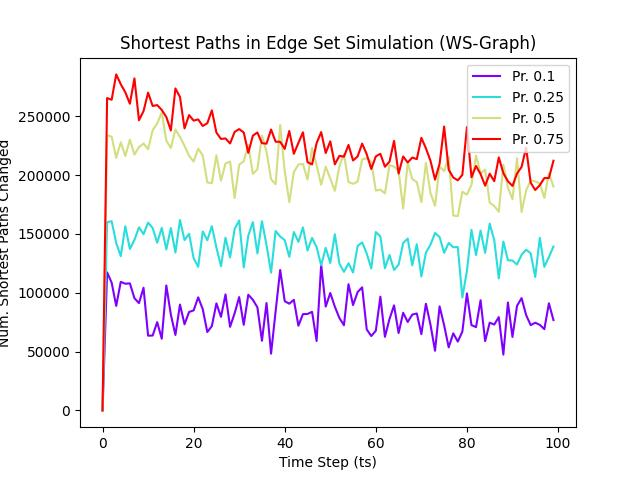
\includegraphics[width=\linewidth]{Figures/esd/paths.jpg}
	\caption{The number of shortest paths changed for \(ts = 100\) time-steps in a WS graph (\(n = 250, k = 10, p = 0.1\)) for a range of probabilities \(Pr_{dyn} = 0.1, 0.25, 0.5, 0.75\). Edge set dynamics. \emph{Produced in Python}}
	\label{fig:esd_paths}
\end{figure}

Figure \ref{fig:esd_paths} shows the number of shortest paths changed at each time step. The results show that the shortest paths are significantly effected by the reassignement of edges, even for relatively low probability values. The number of shortest paths effected scales in proportion to \(Pr_{dyn}\).  \\

\begin{figure}[H]
	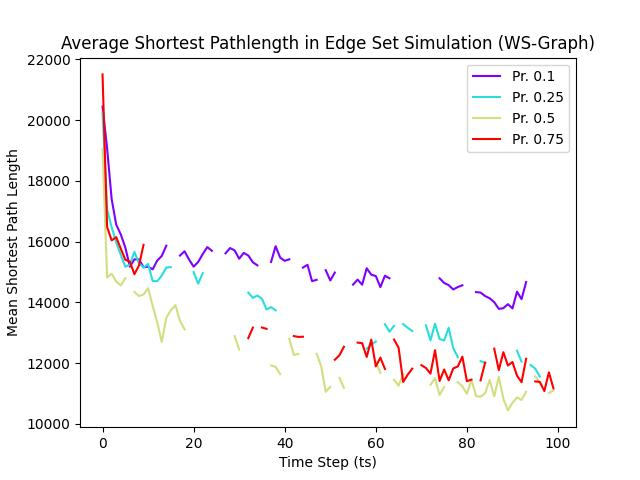
\includegraphics[width=\linewidth]{Figures/esd/lengths.jpg}
	\caption{Average shortest path length for \(ts = 100\) time-steps, for a range of probabilities \(Pr_{dyn} = 0.1, 0.25, 0.5, 0.75\). Edge set dynamics. \emph{Produced in Python}}
	\label{fig:esd_lengths}
\end{figure}

Figure \ref{fig:esd_lengths} shows that the average path length decreases over time. This can be explained by considering the process used to generate WS graphs: The edge-set dynamics continue the uniform random rewiring process. The decrease in shortest path length can be attributed to the consequent transition towards an Erdos-Renyi random graph from the initial WS topology \(G_{0}\). \\

There are also gaps in the analysis seen visually. This results from time-steps where at least one node became disconnected, making some of shortest paths lengths return as \emph{Not a Number} (NaN) in simulations. This simulation identifies that: (a) the proposed edge-set dynamics may alter the statistical properties of the initial topology; (b) for further simulations the connectedness of the toopology must be maintained.  Design of models of topological dynamics that do not denigrate the network statistics is an area warranting further work. \\

In order to maintain the connectedness of the network topology in subsequent simulations, the Edge-Set Dynamics function is modified such that it will not reassign edges connected to vertices with degree one.\\

\subsection{Node Set Dynamics}
Dynamics of the node set are modelled by giving each node in the network some probability \(Pr_{dyn}\) to drop out of the network at each time step. For each time step \(i\), the original topology \(G_{0}\) modified to generate topology \(G_{i}\). If the topology \(G_{i-1}\) is used to seed topology \(G_{i}\) then the number of nodes in the network will quickly approach zero. \\

Having identified that the shortest paths in the network are sensitive to the topological dynamics tested thus far, smaller values of \(P_{dyn}\) are examined with respect to the node set dynamics. \\

\subsubsection{Simulations} 
Taking WS graphs of size \(n = 250\), initial neighbours per-node  \(k = 10\) and rewiring probability \(p = 0.1\), for a range of small probability values \(P_{dyn} = 0.01, 0.05, 0.1\), simulations were conducted for \(ts = 100\) dynamic time steps to ascertain the number of shortest paths changed and the characteristic pathlength. In summary, the results show that just as the number of nodes dropoped out of the network increases in proportion to the probability parameter, so do the number of shortest paths effected: Figure \ref{fig:nsd_paths}. Further, these results show that there is increased variance in the average path length for higher values of \(Pr_{dyn}\), whilst the mean average path length appears to be stable: Figure \ref{fig:nsd_lengths}. \\

\begin{figure}[H]
	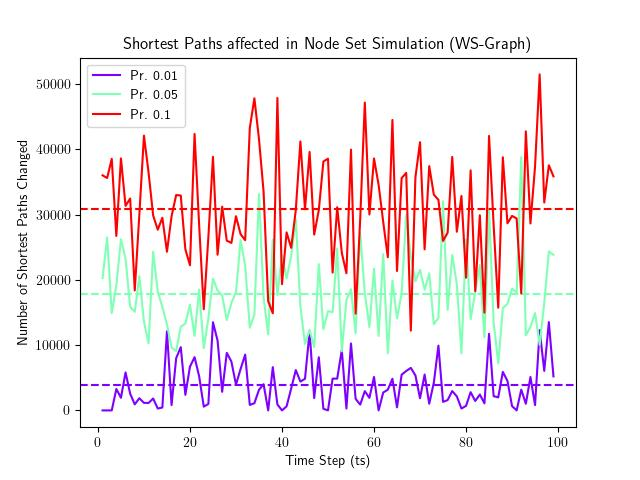
\includegraphics[width=\linewidth]{Figures/nsd/NS_ex1_paths_mean.jpg}
	\caption{Number of shortest paths changed for \(ts = 100\) time-steps of a WS graph. Range of probability values \(Pr_{dyn} = 0.01, 0.05, 0.1\). Node set dynamics. \emph{Produced in Python}}
	\label{fig:nsd_paths}
\end{figure}

\begin{figure}[H]
	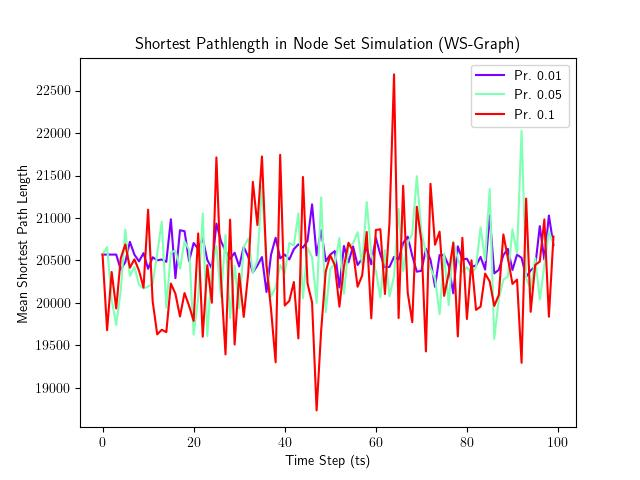
\includegraphics[width=\linewidth]{Figures/nsd/NS_ex3_avg_length.jpg}
	\caption{Average shortest path length for \(ts = 100\) time-steps, for a range of probabilities \(Pr_{dyn} = 0.01, 0.05, 0.1\). Node set dynamics. \emph{Produced in Python}}
	\label{fig:nsd_lengths}
\end{figure}

Examination of the distribution of the count of shortest paths effected for each time step illustrates that in fact the variance increases and the distributions spread out for higher values of \(Pr_{dyn}\) whilst small values (e.g. \(0.01\)) appear to be skewed towards very small changes, following a shape reminiscent of a power-law with a short upper tail: Figure \ref{fig:nsd_dist_prob}. For \(Pr_{dyn} = 0.1\) the number of shortest paths effected at each time-step appears to follow a normal distribution: Figure \ref{fig:nsd_dist}. 

\begin{figure}[H]
	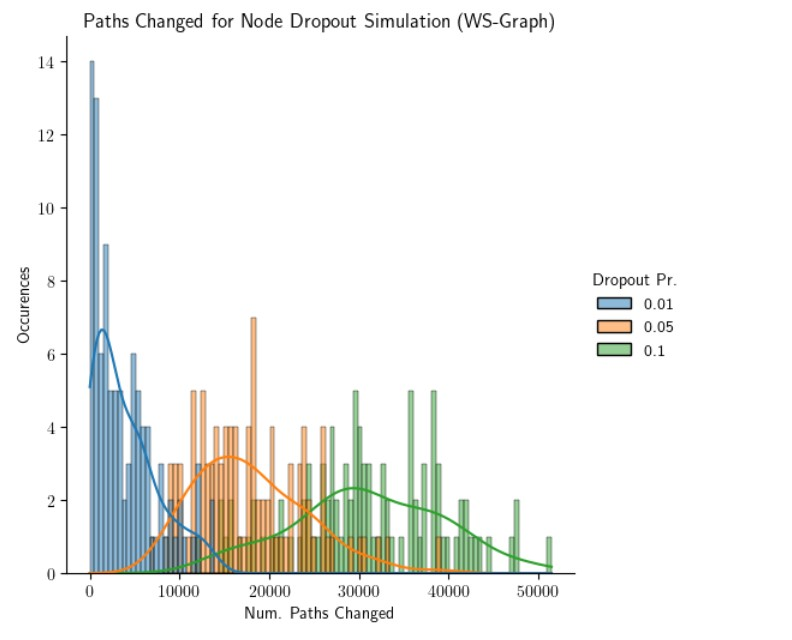
\includegraphics[width=\linewidth]{Figures/nsd/paths_prob_dist.jpg}
	\caption{Distribution of shortest paths changed for a range of \(Pr_{dyn}\) values and Kernel Density Estimate (KDE). Node set dynamics. \emph{Produced in Python}}
	\label{fig:nsd_dist_prob}
\end{figure}

\begin{figure}[H]
	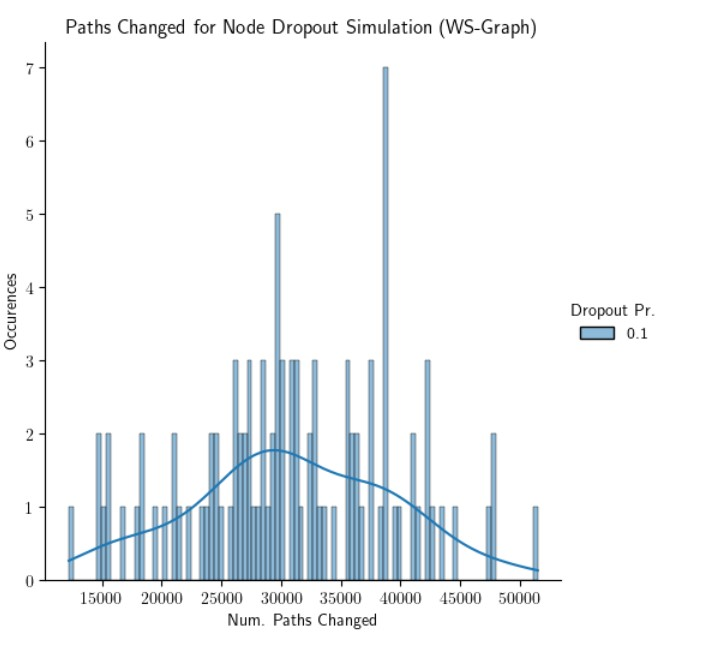
\includegraphics[width=\linewidth]{Figures/nsd/paths_dist.jpg}
	\caption{Distribution of shortest paths changed for a value of \(Pr_{dyn} = 0.1\) and Kernel Density Estimate (KDE). Node set dynamics. \emph{Produced in Python}}
	\label{fig:nsd_dist}
\end{figure}

%------------------------------------------------
\section{Proto-typical Genetic Algorithm for a Simplified Problem Defintion: Travelling Salesman} 

This paper takes an first-principles, incremental approach to development of a GA for the DSPRP. First, an example of a ``proto-typical'' GA is identified in the literature (Mitchell \cite{mitchell:97}). Then, it is applied with minimal adapatations to a relaxed problem definition. The relaxed problem definition is well studied and referred to as the \emph{Travelling Salesman Problem (TSP)}. The GA is then adapted to meet the requirements of a stricter problem definition: the SSSP problem. The same implementation may then be applied to simulations of the DSPRP, however the algorithm is further specialised with immigrant schemes.  \\

Informally, the TSP requires that the least cost path is found in which every vertex of a given fully-connected graph is visited from a given source vertex. The path identified is required to be acyclic. This project does not require paths to return to the source vertex at the end. \\

Genetic Algorithms are based on biological evolution. By the algorithmic processes of selection, crossover and mutation, components of candidate solutions, also referred to as hypotheses, are combined to produce new solutions where the aim is to improve the fitness of the population with each generation. \\

In simple terms, the GA process is as follows: 
\begin{enumerate}
	\item Initialise a population of candidate solutions stochastically 
	\item Evaluate the fitness of all candidates 
	\item Select candidates from the population according to some probably (e.g. probability proportional to fitness) 
	\item Perform crossover with pairs of selected candidates to produce 'child' solutoins which hold a combination of the information from their parents 
	\item Perform a mutation on the child solutions with some probability
	\item Replace the children in the population 
	\item Return to step two 
\end{enumerate} 

\subsubsection{Encoding} Hypohteses need to have representation over which the genetic operators can be applied. Typically, hypohteses are encoded as bit strings \cite{mitchell:97} as in Mitchell's GA. In this implementation the vertices of \(V_{0}\) are denoted with integer labels, and as such the candidate paths are represented as integer lists detailing the order in which vertices are visited. \\

\subsubsection{Hypotheses Generation} Mitchell proposes that in the proto-typical GA bit-strings simply need to be generated at random to initialise the population. Valid hypotheses for the TSP will represent some permutation of the set \(V_{0}\) starting with the source vertex, \(V_{0}(1) = s\). The hypotheses will also have no cycles such that \(\forall i, j \in H [v_{i} \neq v_{j}] \). 

The procedure defined to generate a new candidate solutions is as follows: Generate population size \(p\) permutations of the set of all vertices \(V_{0}\) by shuffling the elements of \(V_{0}\) randomly. The source vertex \(s\) is then removed and replaced at the first index in the list. This generates a set of paths \({P_{i} | i \in {0, 1, ... p}}\) of the form \(P_{i} = {s_{0}, v_{1}, v_{2}, ..., v_{n-1}}\) for \(n\) nodes to visit. \\

\subsubsection{Fitness \& Selection} 
The fitness function of a GA defines the criteria for quantifying the quality of a hypotheses generated. In the context of the TSP, SSSP and DSPRP the aim is to produce hypotheses representing paths about a give network which have the least length. Hence, the fitness function is defined as the inverse of the total pathlength specified by a hypotheses, such that a lesser pathlength corresponds to a greater fitness value Eq \ref{eq:fitness1}. 

\begin{equation}
	f(h_{i}: P(s, r)) = \frac{1}{\sum_{e: (i, j) \in P(s, r)} w_{i, j}}
	\label{eq:fitness1}
\end{equation}

The selection method of a GA effects the average quality of the population by determining the subet of the population at each generation that will be combined to generate the hypotheses of the next generation via the crossover operator. The parallel with natural selection is that parents, the selected hypotheses of the current generation, combine genetic material to create children, the hypotheses of the susbequent generation. For the selection of parents, Mitchell's prototypical GA assigns the probability that a hypothesis will be selected as the ratio of its fitness to the sum fitness of the other hypotheses in the population. This is referred to as fitness proportional or roulette wheel selection. For this implementation, Mitchells design is obeyed and candidates are selected to be parents with probability proportional to their fitness using an equivalent algorithm (Stochastic Universal Sampling (SUS)). (The details of SUS are widely available and trivial and hence excluded from this paper). 

\subsubsection{Crossover} 
The crossover operator combines the information of two ``parent'' hypotheses to produce two new ``child'' hypotheses. The elements at position \(i\) in each child is copied from the element at \(i\) in one of the parents. Mitchell suggests that a prototypical GA will use a crossover method such as single point, two point  or uniform crossover \cite{mitchell:97}. In these methods, the elements are alternated as coming from one parent or the other between uniformly chosen points. For the TSP, it is important that crossover does not produce any cyclic solutions. Hence, this paper proposes to use Order One Crossover (OX1). In OX1, elements from a random index range are taken from one parent and put into one child. Then, the remaining unique values from the alternative parent are inserted in the order in which they appear in the parent. 

\subsubsection{Mutation} 
The mutation operator of a GA makes some stochastic changes to the hypotheses being carried into the next generation, with some probability termed the \emph{mutation rate}, in order to increase the diversity of the population such that it does not converge to local optima. The prototypical mutation scheme presented by Mitchell uniformly chooses and inverts a bit in the hypotheses. For the TSP, a node could be replaced with a randomly selected element of \(V_{0}\) however it this would inevitably lead to an invalid path. Rather, the mutation method has been defined such that two unique indexes in the path are chosen uniformly, and the values at those indexes are swapped. \\

\begin{algorithm}[H]
	\caption{Algorithm 1: Prototypical Genetic Algorithm for the Travelling Salesman Problem}
	\begin{algorithmic}[1]
		\Procedure{GA}{$Fitness, threshold, iterations, graph, p, m, r, s$} 
			\State Fitness: A function that assigns evaluation score given a hypothesis 
			\State threshold: Best of generation fitness value to by achieved before termination 
			\State graph: The graph topology to traverse
			\State s: The starting vertex 
			\State p: Population size (number of hypothese)
			\State r: The fraction of the population to be replaced by Crossover at each step
			\State m: The mutation rate 
			\State Initialise the population: 
				\State \(P \leftarrow\) Generate p permutations of vertex set \(V_{0}\) 
				\State \(P \leftarrow\) Swap values of \(p_{0}, p_{i} = p_{i}, p_{0}\) where \(p_{i} = s\) 
			\State Evaluate: For each $h$ in $P$, compute $Fitness(h)$
			\State $count \leftarrow 0$ 
			\While{$([max_{h} Fitness(h)] < threshold) \land (count < iterations)$} 
				\State Create a new generation, 
				$P_{i}$
				\State (Stochastic Universal Sampling) Select $(1 - r)p$ hypotheses from $P$ to add to $P_{i}$ with fitness proportional probability $Pr(h_{i})$ for hypotheses $h_{i} \in P$ given by: 
					\State \[ Pr(h_{i}) = \frac{Fitness(h_{i})}{\sum_{j=1}^{p} Fitness(h_{j})} \]
				\State (OX1) Select $\frac{rp}{2}$ pairs of hypotheses from P according to $Pr(h_{i})$. 
						\State For each parent pair $(h_{1}, h_{2})$ produce two children $(h_{3}, h_{4})$ and append them to $P_{i}$
					\State (Mutation) Choose $pm$ hypotheses from $P_{i}$ uniformly
						\State For each $h_{i}$ select choose two elements uniformly and swap their values 
					\State Update $P \leftarrow P_{i}$
					\State Update $count \leftarrow (count + 1)$ 
			 \EndWhile  \label{Generation Loop}
		\EndProcedure			
	\end{algorithmic}
	\label{alg:tsp} 
\end{algorithm}

\subsubsection{Simulations} 

From Mitchell's proto-typical GA \cite{mitchell:97} a solution to the TSP has been defined, described formally in Listing \ref{alg:tsp}. The performance of this GA can be ascertained visually: First, a ring lattice (Figure \ref{fig:ring_optimal}) of size \(n = 16\) where each node is connected with it's \(k = 2\) adjacent neighbours is defined. The edge weights in the lattice are set as zero, \(\forall i, j \in V_{0} [w_{ij} = 0]\). Then, edges are added to the ring for all possible pairs of nodes where they do not already exist and excluding self-connections, with a nominally higher weight of \(100\). This produces a fully-connected topology, which can also be conceptualised as a ring lattice of \(n = 16\) and \(k = 15\). \\

\begin{figure}[H]
	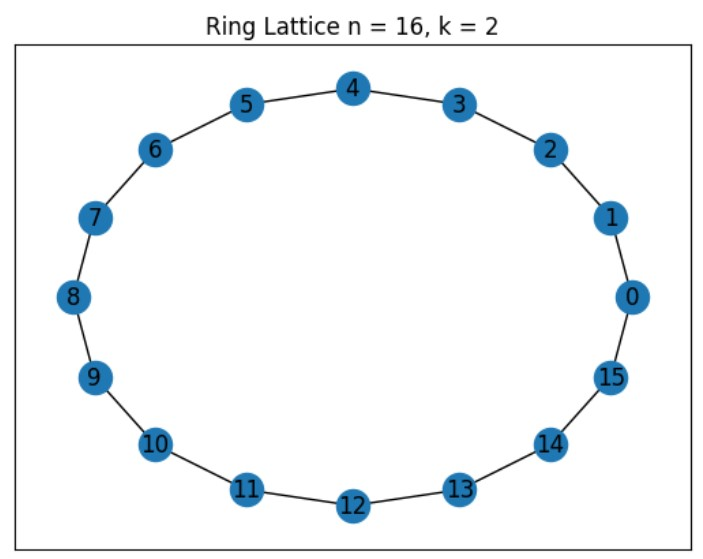
\includegraphics[width=\linewidth]{Figures/tsp/ring_optimal.jpg}
	\caption{Ring lattice with edge weights zero representing the optimal path in the later tested fully-connected topology. \emph{Produced in Python}}
	\label{fig:ring_optimal}
\end{figure}

Clearly, the shortest path to visit all nodes in the network is about the original ring of path cost zero. The distance between the known optimal solution and the solution produced by the GA can be considered as the number of wasted connections where the ring is not obeyed. Consistently, the GA converged to an optimal or near-optimal solution in this setting. Figure \ref{fig:ring_solution} depicts one such solution, where the optimal ring is obeyed with the exception of two wasted connections. \\

\begin{figure}[H]
	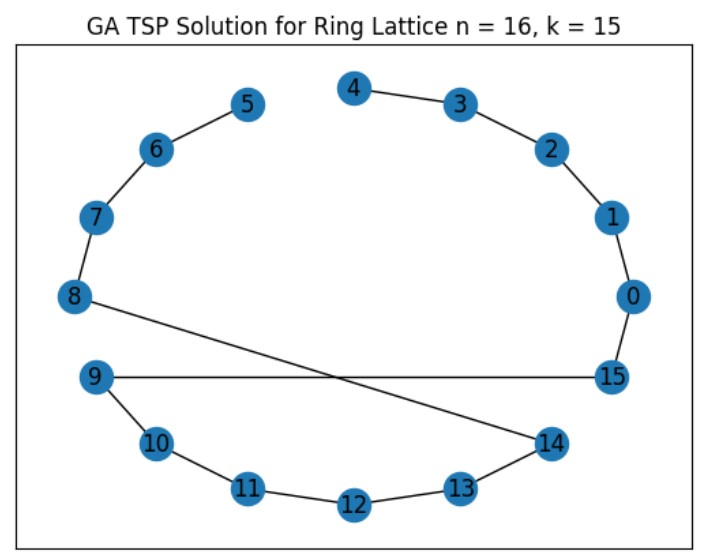
\includegraphics[width=\linewidth]{Figures/tsp/ring_solution.jpg}
	\caption{The path of one solution generated by the GA TSP where the optimal path follows a ring about the nodes, whilst two connections have been wasted. \emph{Produced in Python}}
	\label{fig:ring_solution}
\end{figure}

The learning history of the GA is recorded by the generational mean fitness and maximum fitness, meaning fitness of the best candidate at each generation. Figure \ref{fig:tsp_history} depicts the learning history to achieve the solution presented in Figure \ref{fig:ring_solution}. The generational fitness rises and converges to a maximum of \(0.005\) where it remains. \\

\begin{figure}[H]
	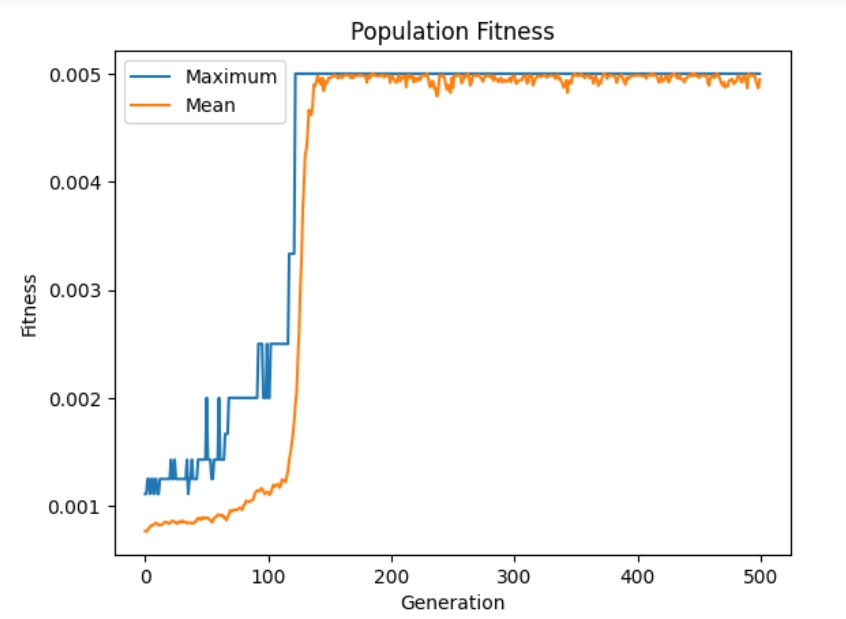
\includegraphics[width=\linewidth]{Figures/tsp/history.jpg}
	\caption{Learning history of the GA for TSP to produce the solution depicted in Figure \ref{fig:ring_solution}. The mean and maximum [best of] generation fitness are plotted. GA converges to a near-optimal solution after ~100 generations. \emph{Produced in Python}}
	\label{fig:tsp_history}
\end{figure}

%------------------------------------------------
\section{Specialised GA for SSSP Routing}

The problem definition can be further restricted to define the SSSP problem. For the SSSP problem the aim become to determine the path \(P_{i} (s, d)\) about the network \(G_{i}\) starting at a source vertex \(s\) and ending on a destination vertex \(d\). Note here that \(d\) represents the destination vertex, whilst \(r\) denotes the reproduction rate, the number of hypohteses selected for crossover, of the GA. Crucially, the TSP requirement that \(G_{i}\) be a fully-connected topology is relaxed: \(G_{i}\) is only required to be a connected topology, such that \(\exists P_{i}(s, d) \forall s, d \in V_{i}, where s \neq d\). \\

In order to solve the SSSP problem, the GA presented in Algorithm \ref{alg:tsp} is modified to meet the new requirements. The destination vertex, \(d\), is taken as an additional parameter. The method of population generation is changed in order to generate random paths \(P_{i} (s, d)\) over the network \(G_{i}\). The genetic operators for crossover and mutation are changed. \\

\subsubsection{Population Generation} In the previous GA, each hypotheses was required to contain each element of the node set \(V_{i}\) exactly once. Edges existed between each possible pair of nodes in the fully-connected topology. Hence, it was sufficient to uniformly permute the set and place the source vertex \(s\) at the first position. However, for the SSSP problem does not mandate a fully-connected topology.
To generate a new hypothesis, the method proposed traverses the graph from the source vertex, uniformly the next vertex from the set of neighbouring vertices at each step, until the destination vertex \(d\) is reached. This method is effectively employed in the literature \cite{yang:10} \cite{yussof:09} \cite{kumar:10}. This process is repeated \(p\) times to generate a population of size \(p\) random hypotheses. 

\subsubsection{Mutation} The mutation method proposed for the SSSP problem utilises the random hypotheses generation method. For a chosen hypotheses \(h_{i}\) one vertex, \(v\) in the path (chromosome) is uniformly selected. The subpath \(v \xrightarrow[subpath]{old} d\) is replaced with a new random subpath \(v \xrightarrow[subpath]{new} d\) giving path \(P_{i} = (s \xrightarrow[subpath]{} v \xrightarrow[subpath]{new} d\).  \\

\subsubsection{Crossover} The crossover method is also used by Yang \& Wang to solve the SSSP problem \cite{yang:10}. Single-point crossover is adopted as described by Mitchell \cite{mitchell:97} and requires that the hypotheses \(h_{a}, h_{b}\) have at least one common vertex. Of the common vertices, one is chosen with uniform probability. Then each hypotheses can be divided by the common vertex \(v\),  \(h_{a}: (s \xrightarrow[h_{a}]{} v) \rightarrow (v \xrightarrow[h_{a}]{} d)\) and \(h_{b}: (s \xrightarrow[h_{b}]{} v) \rightarrow (v \xrightarrow[h_{b}]{} d)\). The crossover operation exchanges the subpaths \((v \xrightarrow[h_{a}]{} d)\) and \((v \xrightarrow[h_{b}]{} d)\) to create two new hypotheses. \\

Initial testing of the specialised algorithm indicates that good performance is possible for small Erdos-Renyi (ER) graphs although results were initially less encouraging for large graphs. For a small ER \(G(n, p)\) graph generated with \(n = 100, p = 0.4\), the learning history shows that the GA improves in fitness with each generation before converging to a short path: Figure \ref{fig:sssp_result_small_1}; Figure \ref{fig:sssp_solution}; Figure \ref{fig:sssp_history_1}. 

% Figure of output from small graph 
% Figure of training in small/large graph 
% Figure of path found in graph 

\begin{figure}[H]
	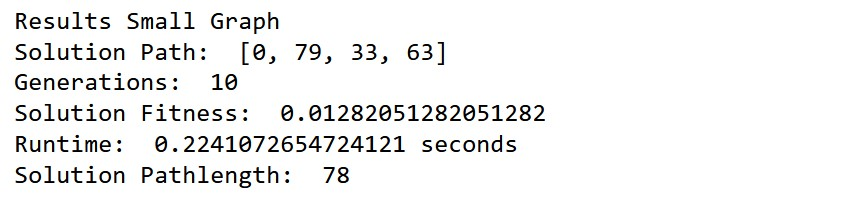
\includegraphics[width=\linewidth]{Figures/sssp/result_small.jpg}
	\caption{Printed output of Specialised GA for an example problem on an ER graph \(n = 100, p = 0.4\) for source and desitnation vertices \(s = 0, d = 63\). (Excl. learning history data).  \emph{Produced in Python}}
	\label{fig:sssp_result_small_1}
\end{figure}

\begin{figure}[H]
	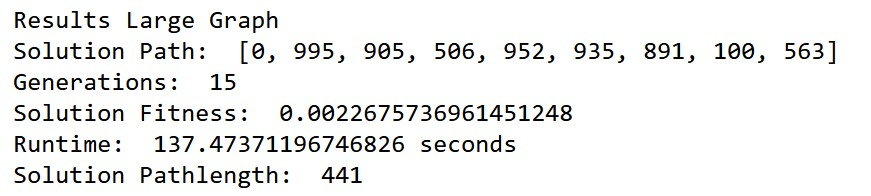
\includegraphics[width=\linewidth]{Figures/sssp/result_large.jpg}
	\caption{Printed output of Specialised GA on an ER graph \(n = 1000, p = 0.4\) for source and desitnation vertices \(s = 0, d = 563\). (Excl. learning history data).\emph{Produced in Python}}
	\label{fig:sssp_result_large}
\end{figure}

\begin{figure}[H]
	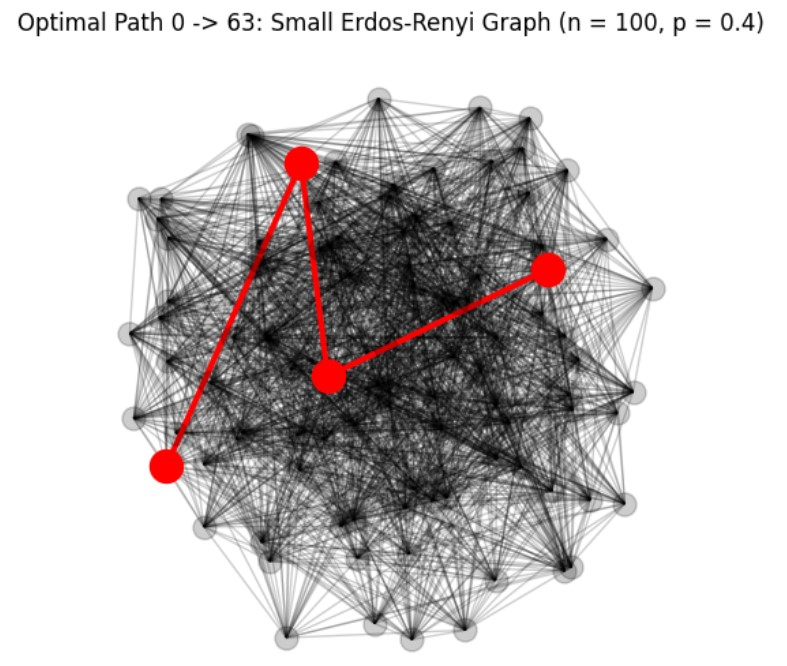
\includegraphics[width=\linewidth]{Figures/sssp/solution.jpg}
	\caption{Example solution path computed with Specialised GA for an ER graph \(n = 100, p = 0.4\). The optimal path found \(SP_{i}(s, d)\) is shown in red. \emph{Produced in Python}}
	\label{fig:sssp_solution}
\end{figure}

\begin{figure}[H]
	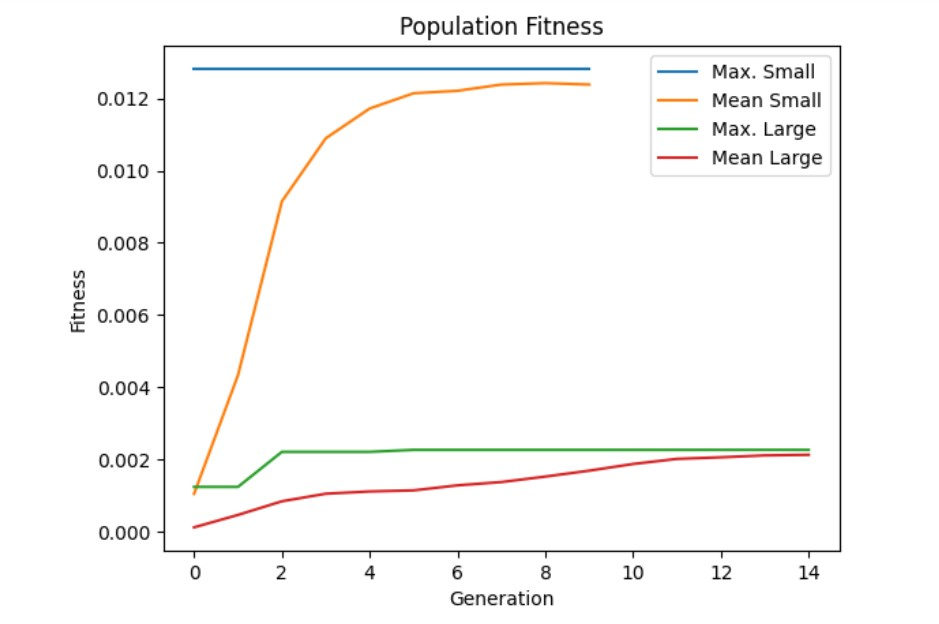
\includegraphics[width=\linewidth]{Figures/sssp/history.jpg}
	\caption{Learning history of the Specialised GA for small ER graph \(n = 100, p = 0.4\) and large ER graph \(n = 1000, p = 0.4\). Mean and maximum of generation fitness is plotted. \emph{Produced in Python}}
	\label{fig:sssp_history_1}
\end{figure}

\subsubsection{Performance Issues} However, the fitness did not improve by as much for an ER graph with \(n = 1000, p = 0.4\): Figure \ref{fig:sssp_history_1}. Futhermore, the solution for a large graph took longer to compute: Figure \ref{fig:sssp_result_large}. Initially, it was considered that the mutation method may scale poorly with the size of the network. In order to rectify and investigate this, an alternative mutation method was proposed,  implemented and investigated. The new method failed to perform as expected in terms of fitness and convergence and did not offer improved runtime: See Figure \ref{fig:mutation_table} and Figure \ref{fig:mutation_comparison} which compare the solution fitness and runtime of the original mutation method (A) and alternative (B) and Best of Generation Fitness (BGF) of (A) and (B) for an exmpale graph, respectively. 

offered simillar fitness and runtime: Figure \ref{fig:sssp_result_small_2}; Figure \ref{fig:sssp_result_large_2}; Figure \ref{fig:sssp_history_2}. \\

\begin{enumerate}
	\item The alternative mutation operator selects a vertex in the path uniformly and replaces it with an alternative vertex that also neighbours the preceeding and succeeding ndoes, producing a new valid path from \((s \rightarrow d)\). 
\end{enumerate}

\begin{figure}[H]
	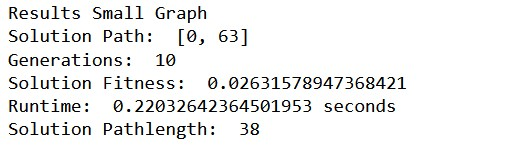
\includegraphics[width=\linewidth]{Figures/sssp/result_small_2.jpg}
	\caption{Printed output of Specialised GA \#2 with alternative mutation method on an ER graph \(n = 100, p = 0.4\) for source and desitnation vertices \(s = 0, d = 63\). (Excl. learning history data).\emph{Produced in Python}}
	\label{fig:sssp_result_small_2}
\end{figure}

\begin{figure}[H]
	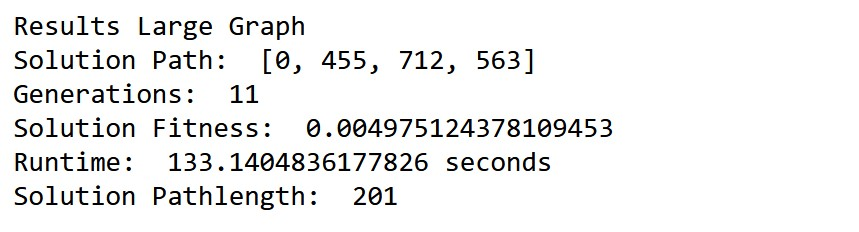
\includegraphics[width=\linewidth]{Figures/sssp/result_large_2.jpg}
	\caption{Printed output of Specialised GA \#2 with alternative mutation method on an ER graph \(n = 1000, p = 0.4\) for source and desitnation vertices \(s = 0, d = 563\). (Excl. learning history data).\emph{Produced in Python}}
	\label{fig:sssp_result_large_2}
\end{figure}

\begin{figure}[H]
	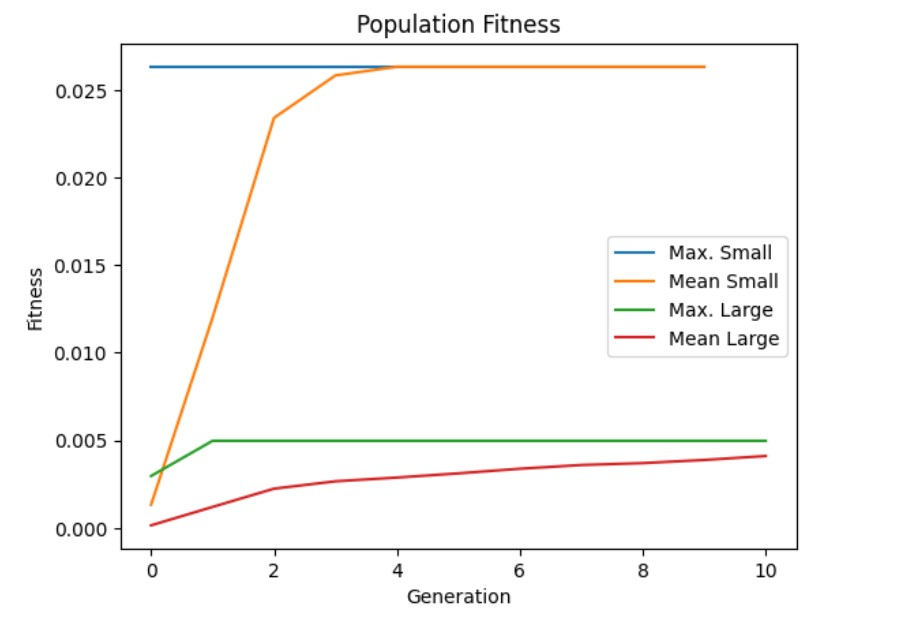
\includegraphics[width=\linewidth]{Figures/sssp/history_2.jpg}
	\caption{Learning history of the Specialised GA \#2 with alternative mutation method for small ER graph \(n = 100, p = 0.4\) and large ER graph \(n = 1000, p = 0.4\). Mean and maximum of generation fitness is plotted\emph{Produced in Python}}
	\label{fig:sssp_history_2}
\end{figure}

\begin{figure*}
	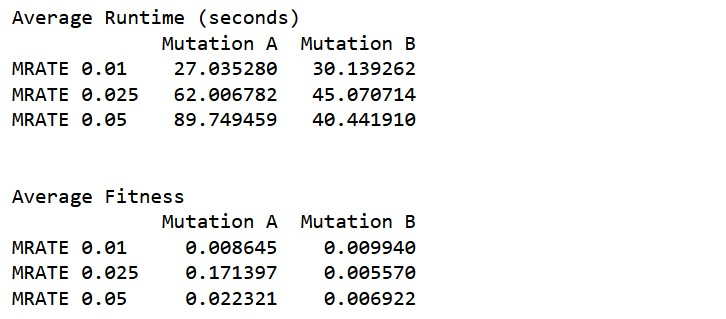
\includegraphics[width=\linewidth]{Figures/sims/mutation/mutation_table.jpg}
	\caption{Mean runtime and solution (converged) fitness for a range of mutation rates with the original (A) and alternative (B) mutation methods. A: Produce a new random subpath from a vertex \(v\) to destination; B: Uniformly replace a single vertex in path .  \emph{Produced in Python}}. 
	\label{fig:mutation_table}
\end{figure*}

\begin{figure*}
	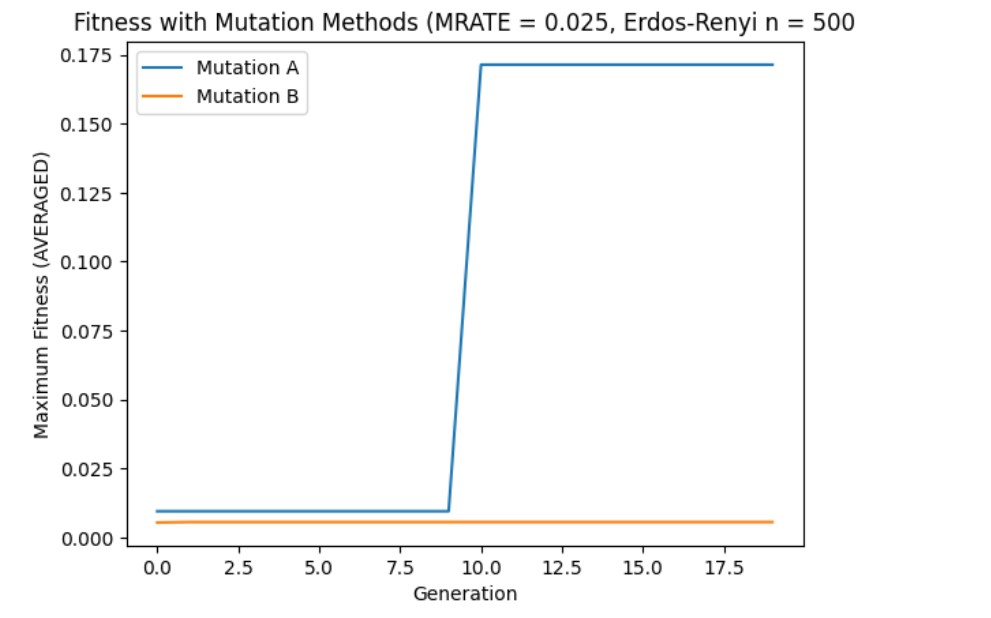
\includegraphics[width=\linewidth]{Figures/sims/mutation/mutation_comparison.jpg}
	\caption{Mean Best of Generation Fitness (BGF) for two mutationa methods: The original (A) and alternative (B). A: Produce a new random subpath from a vertex \(v\) to destination; B: Uniformly replace a single vertex in path . The original Mutation A performs as expected whilst Mutation B fails to converge. \emph{Produced in Python}}. 
	\label{fig:mutation_comparison}
\end{figure*}

Then, it was hypothesised that as the mutation method and population generation utilise the same random path generation algorithm, that is could be this algorithm and consequently the both the mutation method and population generation that scale poorly with large graphs. Intuitively, traversing a graph at random until landing on a desired vertex is likely to require more iterations for a large graph. This hypothesis was confirmed by running the Specialised GA for graphs of increasing size and recording the time taken to generate the initial population and time taken to converge the GA separately: Figure \ref{fig:sssp_runtime}. 

\begin{figure}[H]
	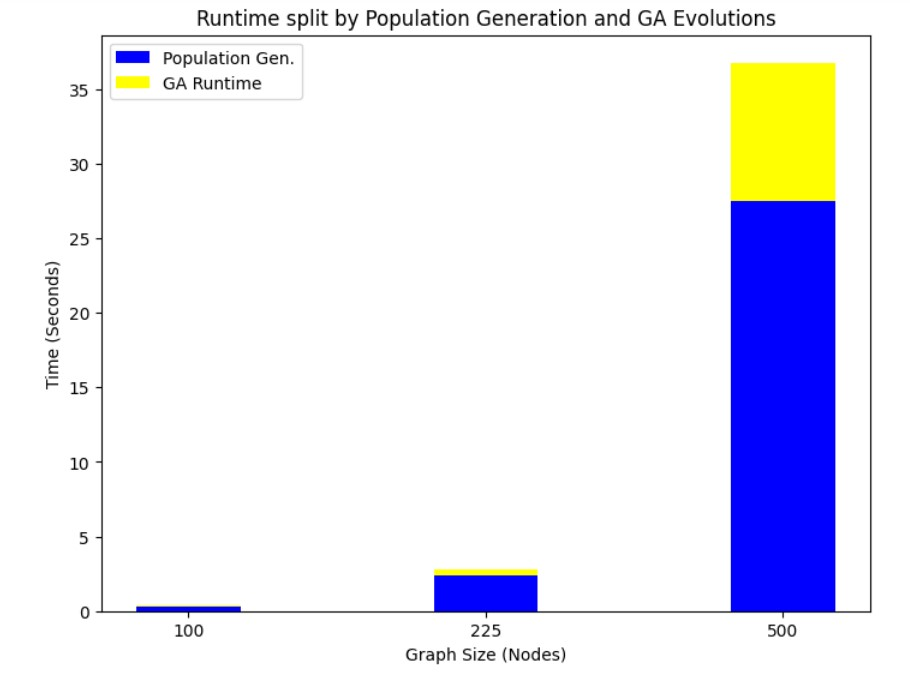
\includegraphics[width=\linewidth]{Figures/sssp/runtime.jpg}
	\caption{Runtime of the Specialised GA by population generation (blue) and convergence (yellow) for ER graphs of increasing size. This plot clearly shows that initial population generation is the most time consuming stage of the GA which also scales poorly with the size of the network. \emph{Produced in Python}}
	\label{fig:sssp_runtime}
\end{figure}

%------------------------------------------------
\section{Specialised GA with Immigrant Schemes for DSPRP} 

% Explain immigrant schemes (elitist) 
% Pseudocode GA with immigrant schemes 
% Show some initial results 
For DOPs, GAs may fail to converge as changing environments require the GA to maintain a higher population diversity in order to adapt new search space and optimum. The process of convergence is itself a process of reducing the population diversity as the hypotheses become increasingly simillar to a desired optimum. Hence, a partially converged population may be less tolerant to change and struggle to evolve towards a new optimum. \\

To address this problem, Immigrant Schemes have been proposed \cite{yang:10}. The Random Immigrant GA (RIGA) was proposed by Grefenstette \cite{}. The random immigrants scheme inserts a small set of new random hypotheses to the population at each generation. These \emph{random immigrants} replace either the uniformly selected hypotheses in the population, or the least fit hypotheses in the population. This paper adopts the later strategy.  \\

However, in a slowly changing environment where maintenance of diversity is less important the introduced random immigrants may disrupt convergence towards the global optimum and degrade performance \cite{yang:10}. Where the severity of changes is small, the existing solutions may still be fit in the new environment if few or no shortest paths are affected. Based on this consideration for dynamic environments, Yang \& Wang investigate elitism based immigrants GA (EIGA) \cite{yang:10}. The Hybrid Immigrants GA (HIGA) utilises the immigrant schems of both RIGA and EIGA. \\

This paper investigates the introduction of random, elitism and hybrid immigrants into the population maintained by the Specialised GA for the SSSP, in an attempt to improve performance in DSPRP simulations. Yang \& Wang demonstrated improved performance over a standard GA with RIGA, EIGA and HIGA for dynamic environments. The ratio of the number of immigrants to the size of the population is set at \(0.2\) in this paper as in \cite{yang:10} for RIGA, EIGA and HIGA. In the HIGA, the set of immigrants at each generations consists of \(0.1 * p\) Random Immigrants and \(0.1 * p\) Elitism Immigrants. \\

The EIGA is specified by Yang \& Wang as follows: For each generation \(i\) the `elite' most fit hypothesis from the previous generation \(P_{t-1}\), denoted \(E_{t-1}\), is mutated with with some probability \(P_{i}^{m}\), \(ei * p\) times where \(ei\) is the fraction of the population to replace with elitism immigrants. In the case where \(E_{t-1}\) is not mutated, a copy of \(E_{t-1}\) itself is inserted into the immigrant population. In this paper, the elitism mutation probability \(P^{i}_{m}\) is set at \(0.8\) as in Yang \& Wang \cite{yang:10} in order to have few relatively few copies of \(E_{t-1}\) and increased diversity within the EIGA, considering that the prevoius simulations indicated turbulent dynamic environments for even small change probabilities. \\

This paper proposes to run DSPRP simulations with the RIGA, EIGA and HIGA variants of the Specialised GA. Pseudocode is provided in \textbf{Algorithm 2}. 


\begin{algorithm}[H]
	\caption{Algorithm 2: Specialised Genetic Algorithm with Immigrant Schemes}
	\begin{algorithmic}[1]
		\Procedure{GA}{$Fitness, threshold, iterations, graph, p, m, r, s$} 
			\State \textbf{Input} $ri, ei, im, random, elite$ 
			\State Fitness: A function that assigns evaluation score given a hypothesis 
			\State threshold: Number of generations with unchanged maximum fitness before termination
			\State graph: The graph topology to traverse
			\State s: The starting vertex 
			\State p: Population size (number of hypothese)
			\State r: The fraction of the population to be replaced by Crossover at each step
			\State m: The mutation rate 
			\State ri: Fraction of population to replace with random immigrants
			\State ei: Fraction of population to replace with elitist immigrants
			\State im: Probability to mutate elitist immigrants 
			\State random: Boolean flag to inject random immigrants 
			\State elite: Boolean flag to inject elitism immigrants 
			\State Initialise the population: 
				\State \(P \leftarrow\) Generate p random paths \((s \rightarrow d)\) 
			\State Evaluate: For each $h$ in $P$, compute $Fitness(h)$
			\State $count \leftarrow 0$ 
			\State $unchanged \leftarrow 0$ 
			\While{$(unchanged < threshold) \land (count < iterations)$} 
				\State Create a new generation, $P't$
				\State (Stochastic Universal Sampling) Select $(1 - r)p$ hypotheses from $P$ to add to $P't$ with fitness proportional probability $Pr(h_{i})$ for hypotheses $h_{i} \in P$ given by: 
					\State \[ Pr(h_{i}) = \frac{Fitness(h_{i})}{\sum_{j=1}^{p} Fitness(h_{j})} \]
				\State (Crossover) Select $\frac{rp}{2}$ pairs of hypotheses from P according to $Pr(h_{i})$. 
						\State For each parent pair $(h_{1}, h_{2})$ produce two children $(h_{3}, h_{4})$ and append them to $P_{i}$:
							\State Uniformly select a vertex \(v\) from the set of common vertices\(\gamma \leftarrow x, \forall x \in h_{1} \land x \in h_{2}\) 
							\State Define two children $h_{3}: (s \rightarrow[h_{1}] v \rightarrow[h_{2}] d)$ and $h_{4}: (s \rightarrow[h_{2}] v \rightarrow[h_{1}] d)$ 
					\State (Mutation) Choose $pm$ hypotheses from $P_{i}$ uniformly
						\State For each $h_{i}$ uniformly choose a vertex \(v \in h_{i}, v \neq d\) in the path \((s \rightarrow v \rightarrow d)\) and replace the subpath \((v \rightarrow d)\) with a new random subpath \((v \rightarrow[rnd] d)\).	
		\EndWhile  
	\EndProcedure
	\end{algorithmic}
	\label{alg:higa} 
\end{algorithm}
\begin{algorithm}[H]
	\begin{algorithmic}[30]
					\State Evaluate the interim population $P't$
					\State $E(t-1) \leftarrow$ The `elite' highest-fitness hypothesis from the previous generation $P(t-1)$ 
					\If{$elite$}
						\If{$E(t -1)$ is not a valid path in $G_{t}$}
							\State Utilise the fittest hypothesis of the current population: 
							\State $E(t - 1) \leftarrow \max_{h \in P} Fitness(h)$ 
						\EndIf
						\State Generate $ei * p$ elitism immigrants by mutating $E(t-1)$ with probability $im$ 
						\State Evaluate elitism immigrants 
					\EndIf
					\If{$random$}
						\State Generate $ri * p$ random immigrants by generating new random paths \((s \rightarrow d)\) 
						\State Evaluate random immigrants 
					\EndIf
					\State Replace the $((ei * p) + (ri * p))$ least fit hypotheses from interim population $P't$ with the immigrant hypotheses 
					
					\If{$\max_{h \in P} Fitness(h) = \max_{h \in P't} Fitness(h)$}
						\State Update $unchanged \leftarrow (unchanged + 1)$
					\Else 
						\State Update $unchanged \leftarrow 0$ 
					\EndIf
					\State Update $P \leftarrow P't$
					\State Update $count \leftarrow (count + 1)$ 		
	\end{algorithmic}
	\label{alg:higa} 
\end{algorithm}

%------------------------------------------------
\section{Basic Simulation Results \& Analysis} 



\subsection{Defining Optimal Parameters} 

First, simulations are run on static topologies to investigate the population size and mutation rate that encourage convergence and maximum generation fitness. 

\subsubsection{Simulation 1} Log-Normal (LN), Watts-Strogatz (WS) and Barabasi-Albert (BA) models of the maximum size \(n = 500\) considred in this paper are selected as representatives to investigate the required population size for good results. 

Initially,  population sizes \(50, 75, 100\) hypotheses are investigated for Log-Normal graphs of size \(100, 225, 500\) nodes. Ten runs of the GA are committed with new graphs for each configuration of population and network size and the average of results are taken. The mean best-of-generation fitness (BGF) is plotted, revealing that the best performance on average is achieved for population size \(100\): Figure \ref{fig:pop_1}. 

\begin{figure*}
	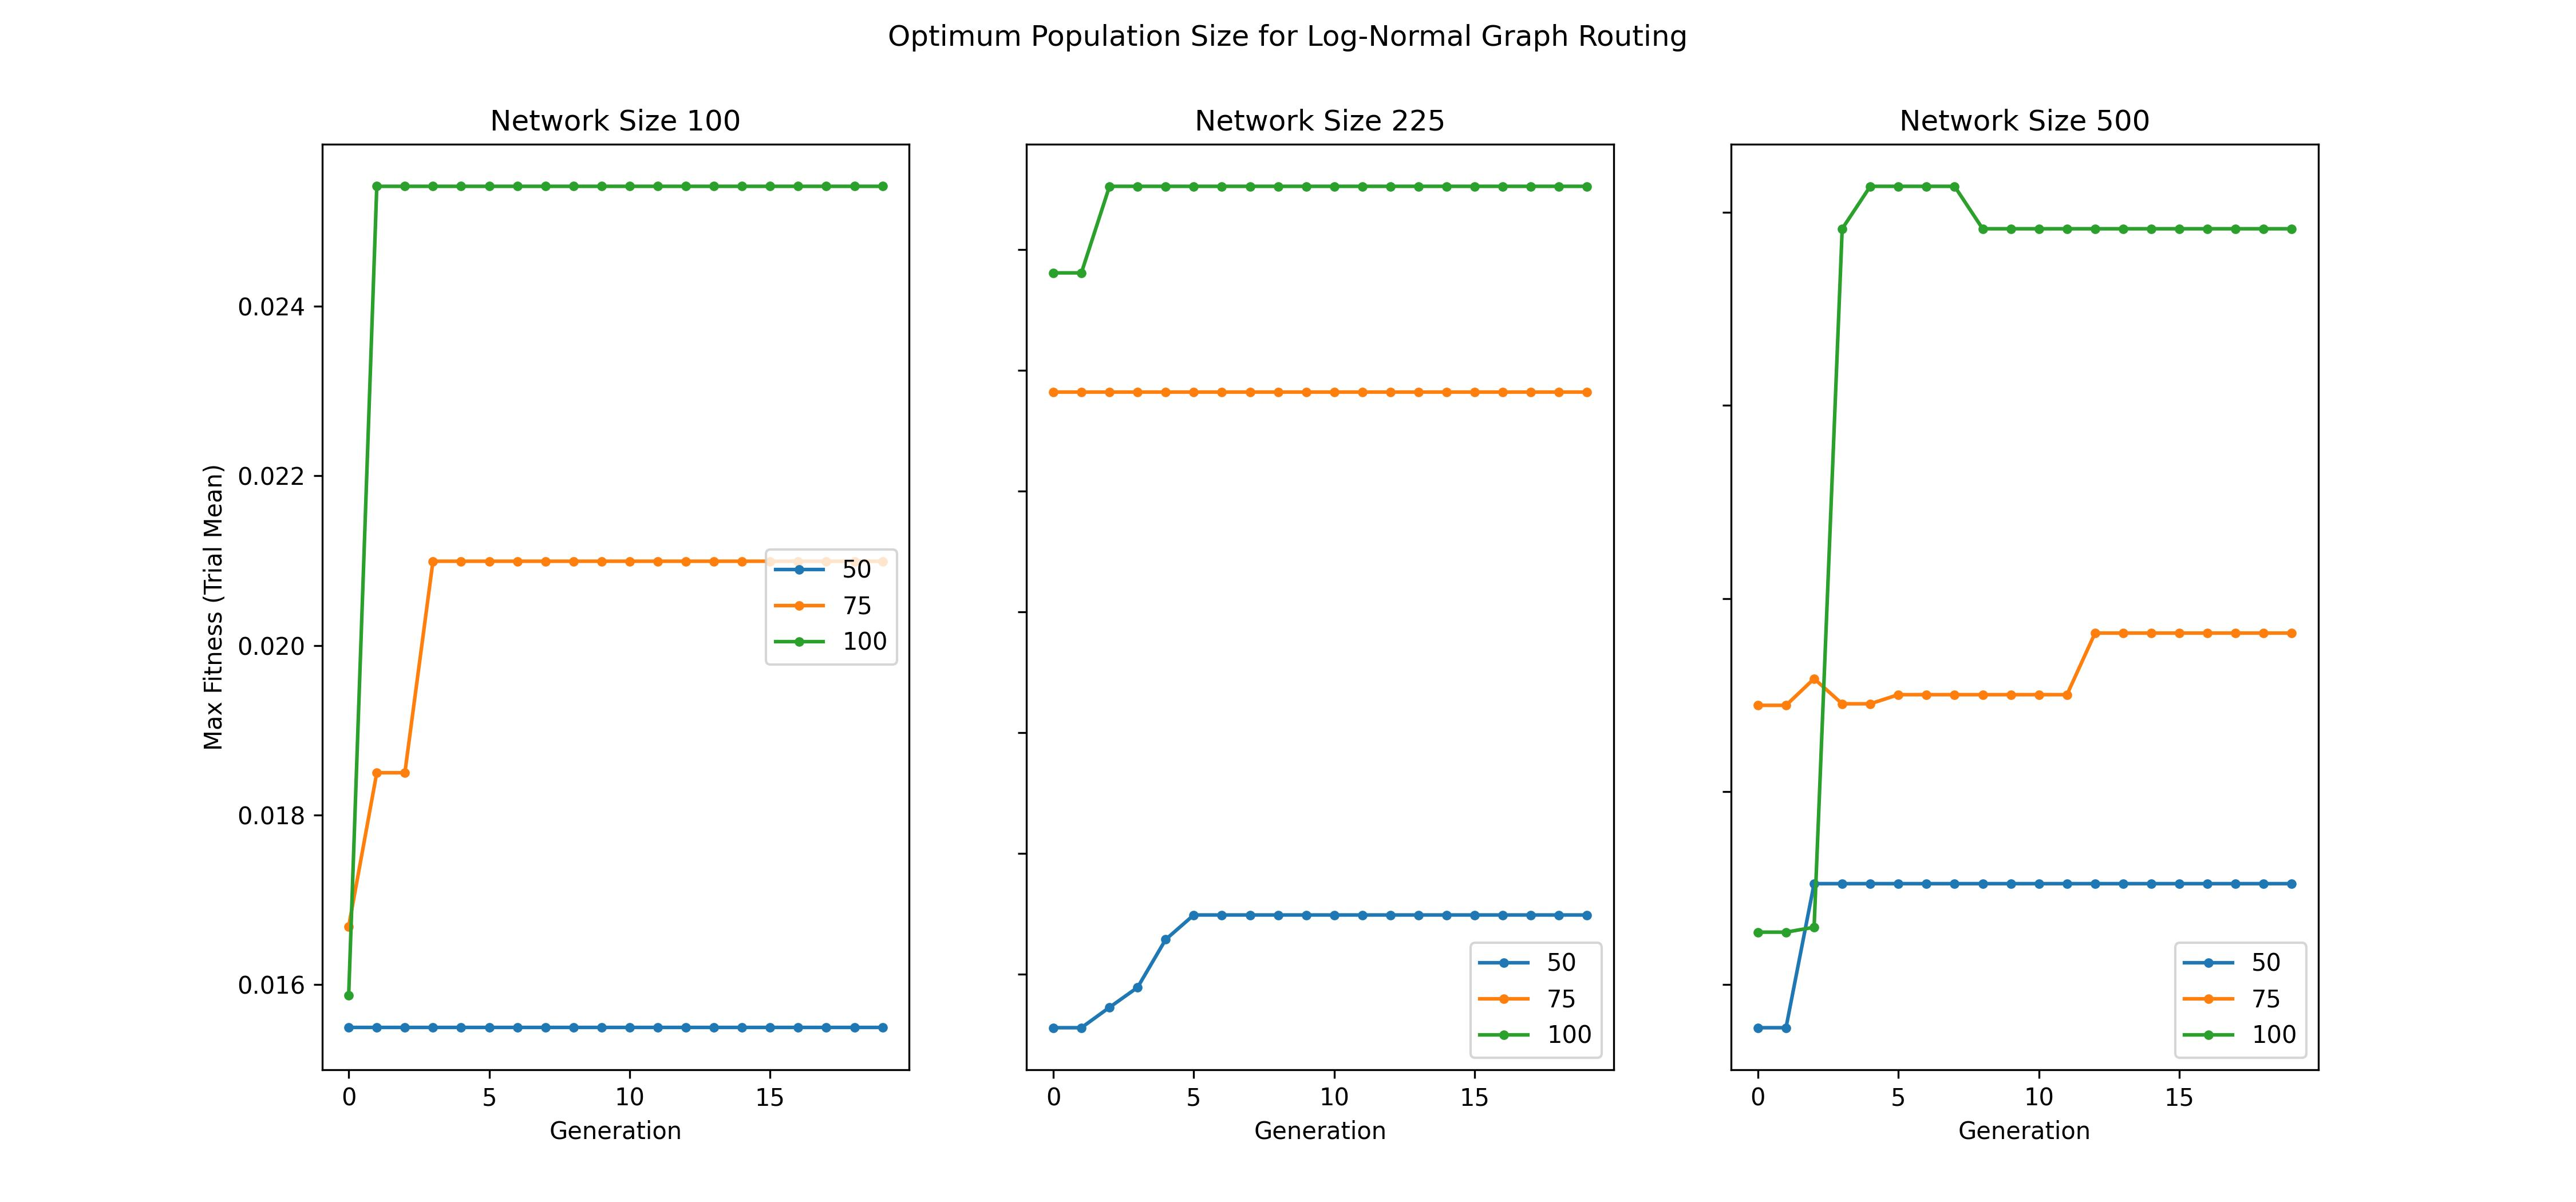
\includegraphics[width=\linewidth]{Figures/sims/population/lognormal.jpg}
	\caption{BGF with population sizes \(50, 75, 100\) with random LN graphs of sizes \(100, 225, 500\) nodes. Mean of 10 runs. This simulation shows that population size \(100\) gives better performance on average. \emph{Produced in Python}}. 
	\label{fig:pop_1}
\end{figure*}

Based on the improved performance with population size \(100\) a further simulation was conducted to ascertain whether further increasing the population size would be beneficial: Figure \ref{fig:ln_500}. For LN 500 node graphs randomly generated for each trial, the population sizes \(100, 110, 120\) were evaluted. The mean BGF of ten trials is taken for presentation. Population size \(100\) gave higher BGF on average. 

\begin{figure}[H]
	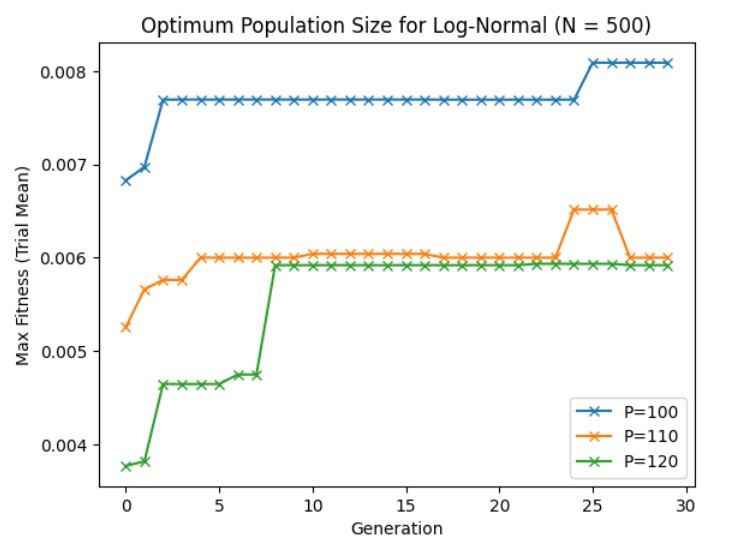
\includegraphics[width=\linewidth]{Figures/sims/population/ln_500.jpg}
	\caption{BGF with population sizes \(100, 110, 120\) with LN graphs of size \(n = 500\). Mean of 10 runs. This simulation shows that population size \(100\) gives better performance on average. \emph{Produced in Python}}. 
	\label{fig:ln_500}
\end{figure}

Following from this affirmation for a population size of \(100\) hypotheses, a set of similar simulations were conducted with WS, BA and LN 500 node topologies to confirm that the results are consistent for each topology. The graph size of \(500\) nodes is chosen as representative considering that: (1) Results for \(100, 225, 500\) nodes were consistent for LN graphs; (2) Larger graphs present a larger search space and are therefore more likely to show poor performance and set the requirement for the population size.\\

The results in Figure \ref{fig:all_pop} confirm that the population size \(100\) is optimal except for in WS graphs for which population size \(75\) performs better.\\

\begin{figure*}
	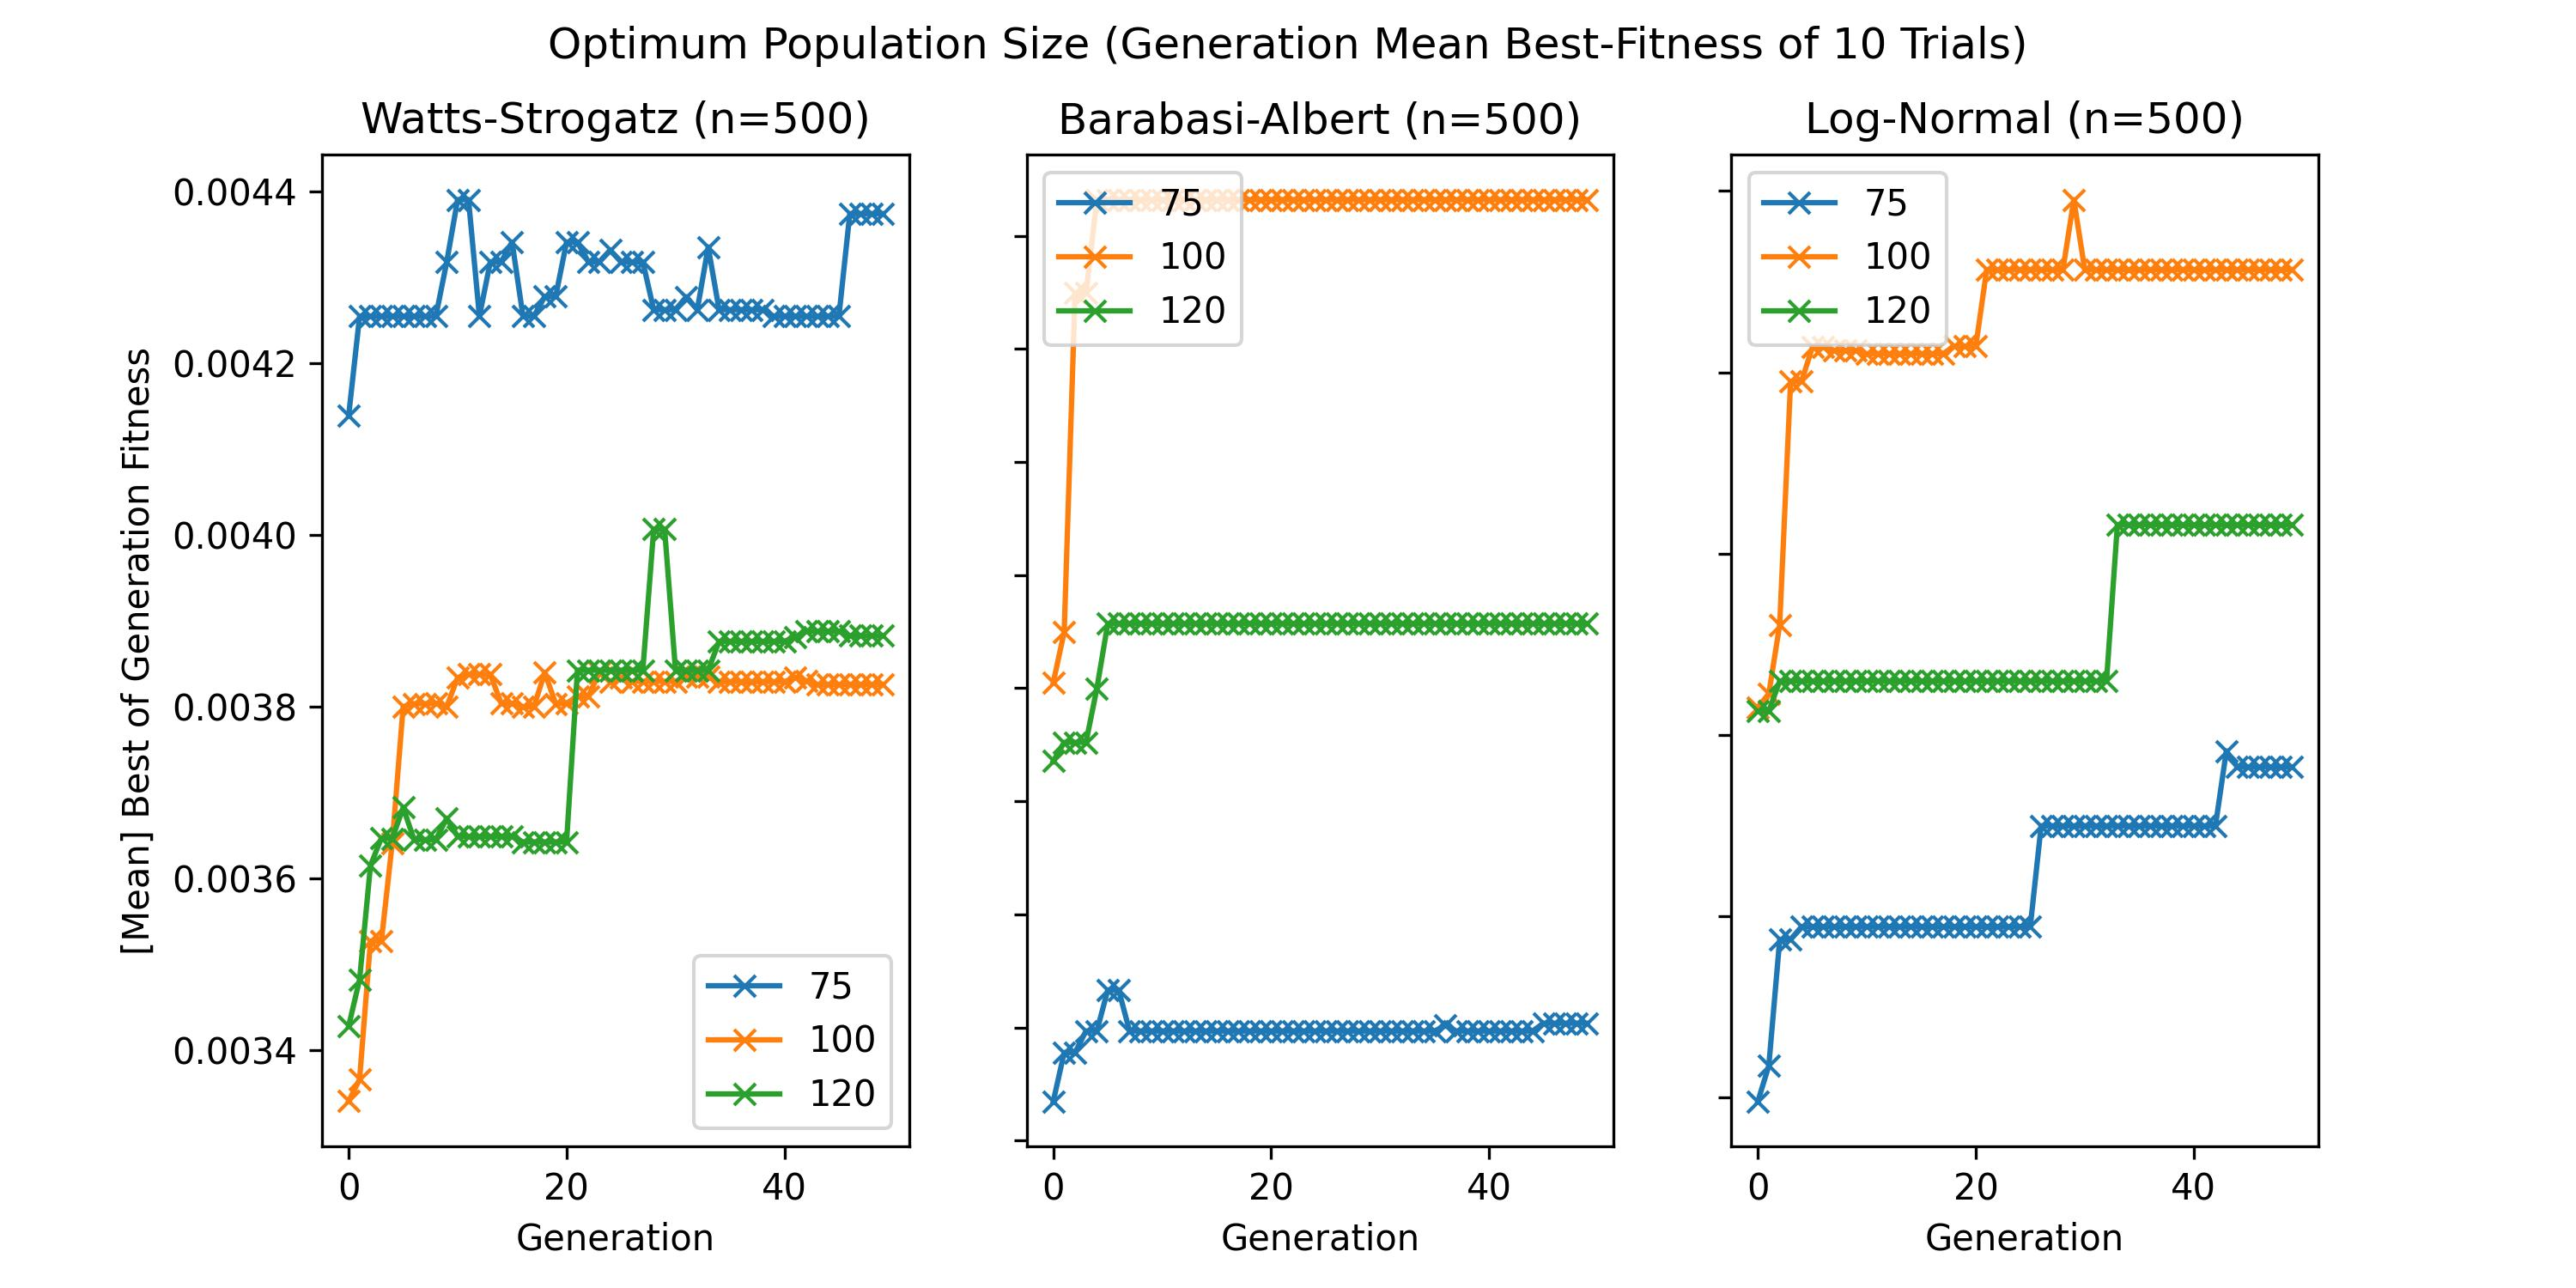
\includegraphics[width=\linewidth]{Figures/sims/population/all_pop.jpg}
	\caption{BGF with population sizes \(75, 100, 120\) with random WS, BA, LN graphs of size \(n = 500\). Mean of 10 runs. Population size \(100\) gives better performance on average except in WS graphs. \emph{Produced in Python}}. 
	\label{fig:all_pop}
\end{figure*}

The mean Best of Generation Fitness (BGF) of ten trials is taken for Figure \ref{fig:all_pop}, Figure \ref{fig:ln_500}. For each trial, a new random graph of the given parameters is generated and each variation of the GA with different population sizes is run on the same topology for that trial such that the average BGF is comparable. \\ 

These simulations indicate that the overall optimum population size for the SSSP GA is \(100\) hypotheses. However, performance may be improved in strong Small-Worlds by reducing the population size by a quater. Further to this, it was considered that for Immigrant GAs an increased population size may be beneficial to account for the fraction of the population replaced at each generation. Figure \ref{fig:higa_pop} illustrates the mean BGF of ten runs of the HIGA for a LN 500 graph (3000 edges). Population size \(100\) performed best on average. \\

\begin{figure}[H]
	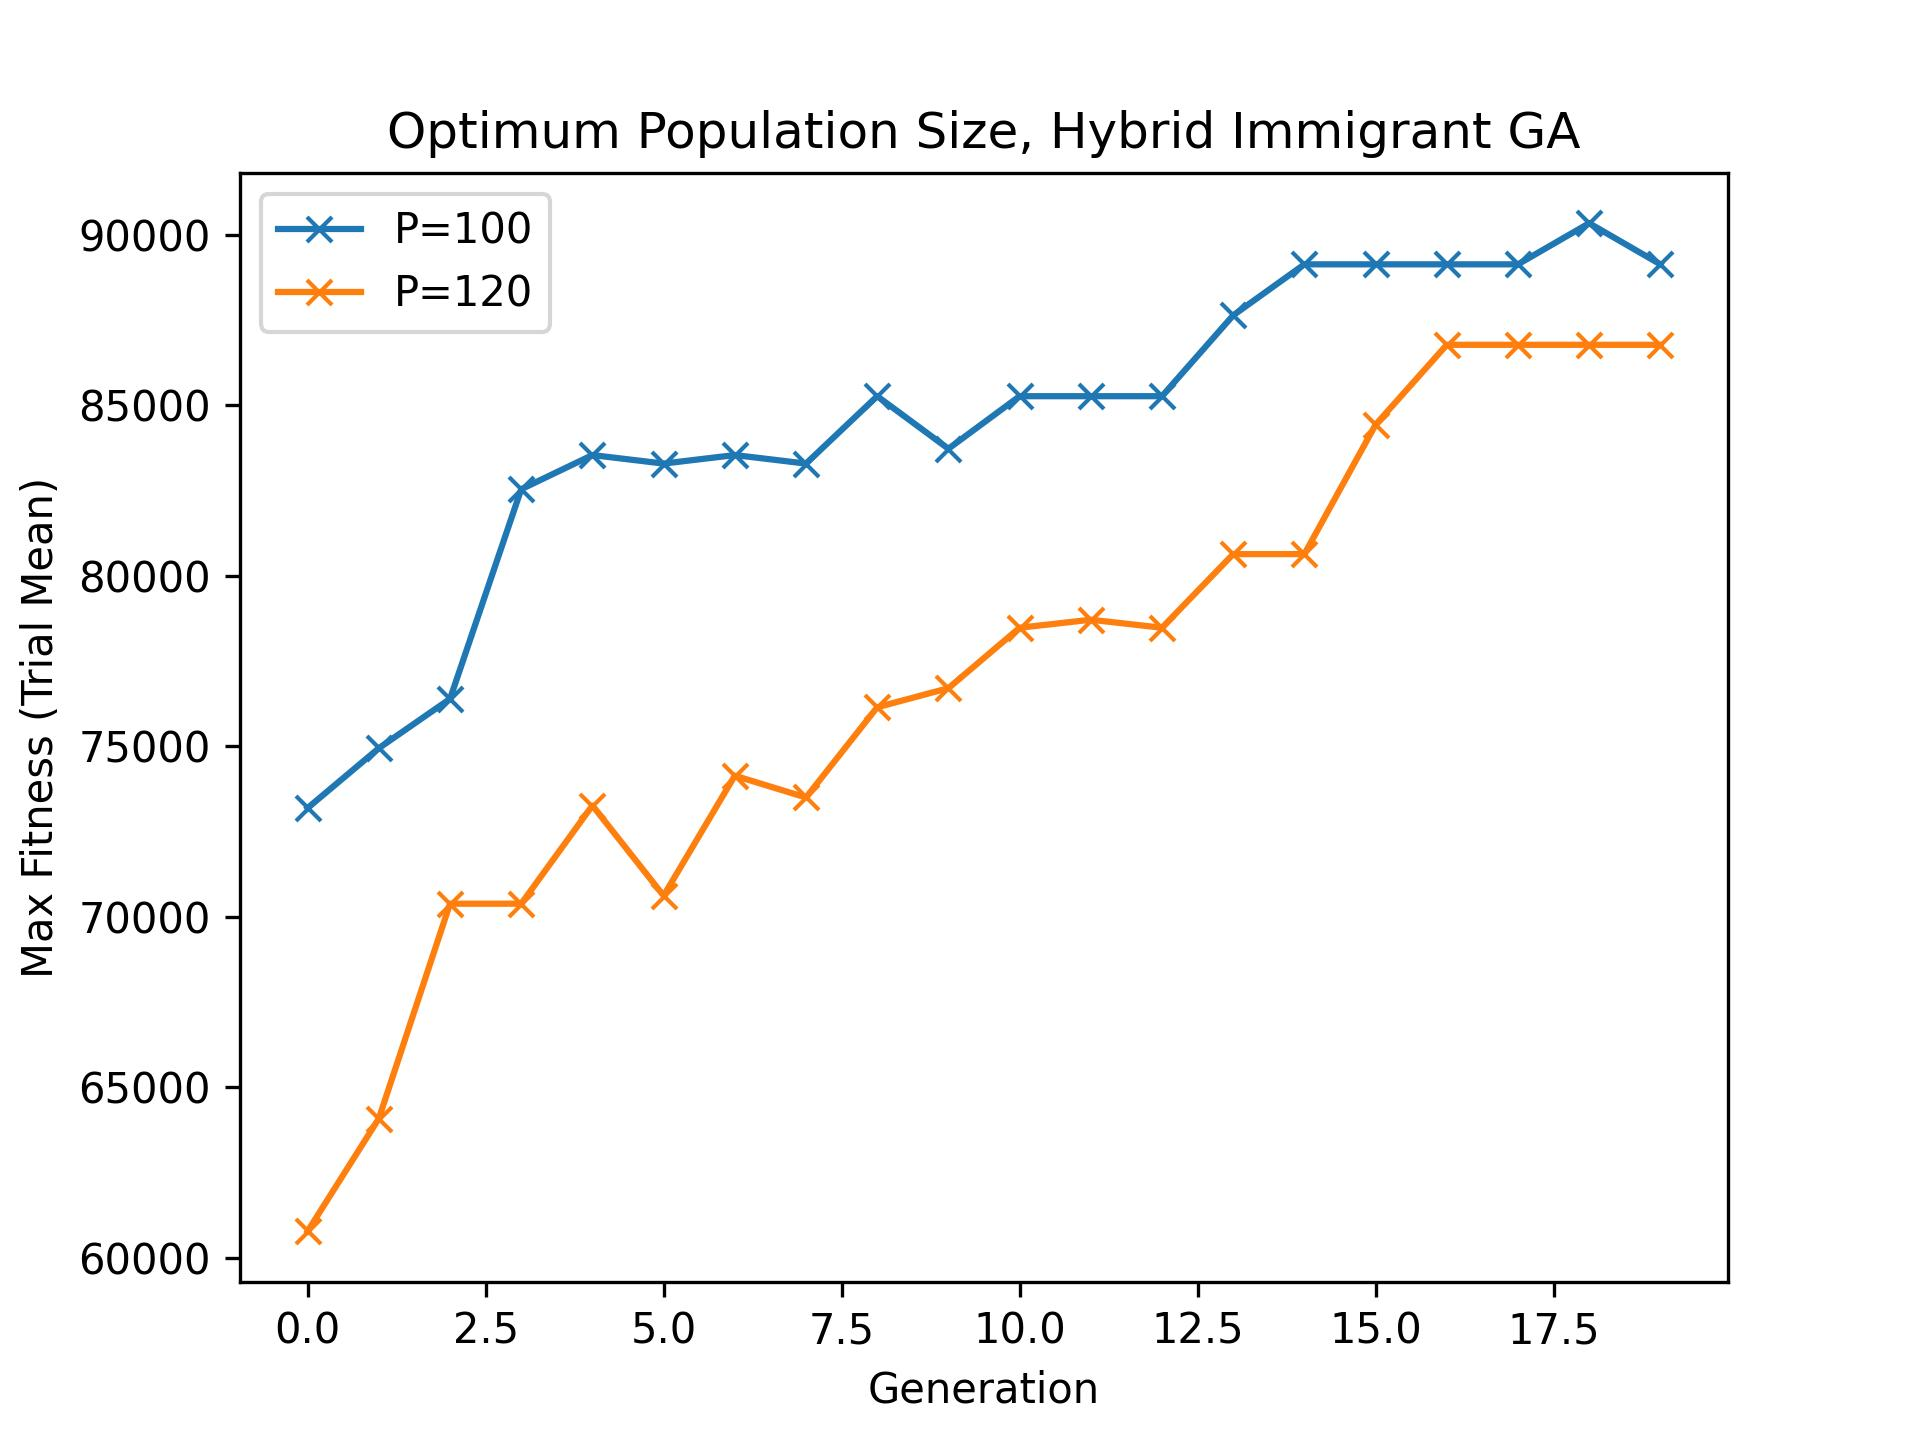
\includegraphics[width=\linewidth]{Figures/sims/population/higa_pop.jpg}
	\caption{Mean BGF of ten trials with population sizes \(100, 120\) over random LN graph \(n = 500, degree = 3000\). Population size \(100\) gives better performance. \emph{Produced in Python}}. 
	\label{fig:higa_pop}
\end{figure}

\subsubsection{Simulation 2} This set of simulations seeks to identify the optimum \(mutation rate\) for static topologies, given the optimum population size \(100\). LN graphs of sizes \(100, 225, 500\) are chosen. Mutation rates \(0.02, 0.025 and 0.03\) are investigated. Figure \ref{fig:mutation_opt} shows the mean BGF of three trials and the results are variable. Figure \ref{fig:mutation_opt_2} shows a repeat of this simulation where the mean BGF is taken of ten trials. 

\begin{figure*}
	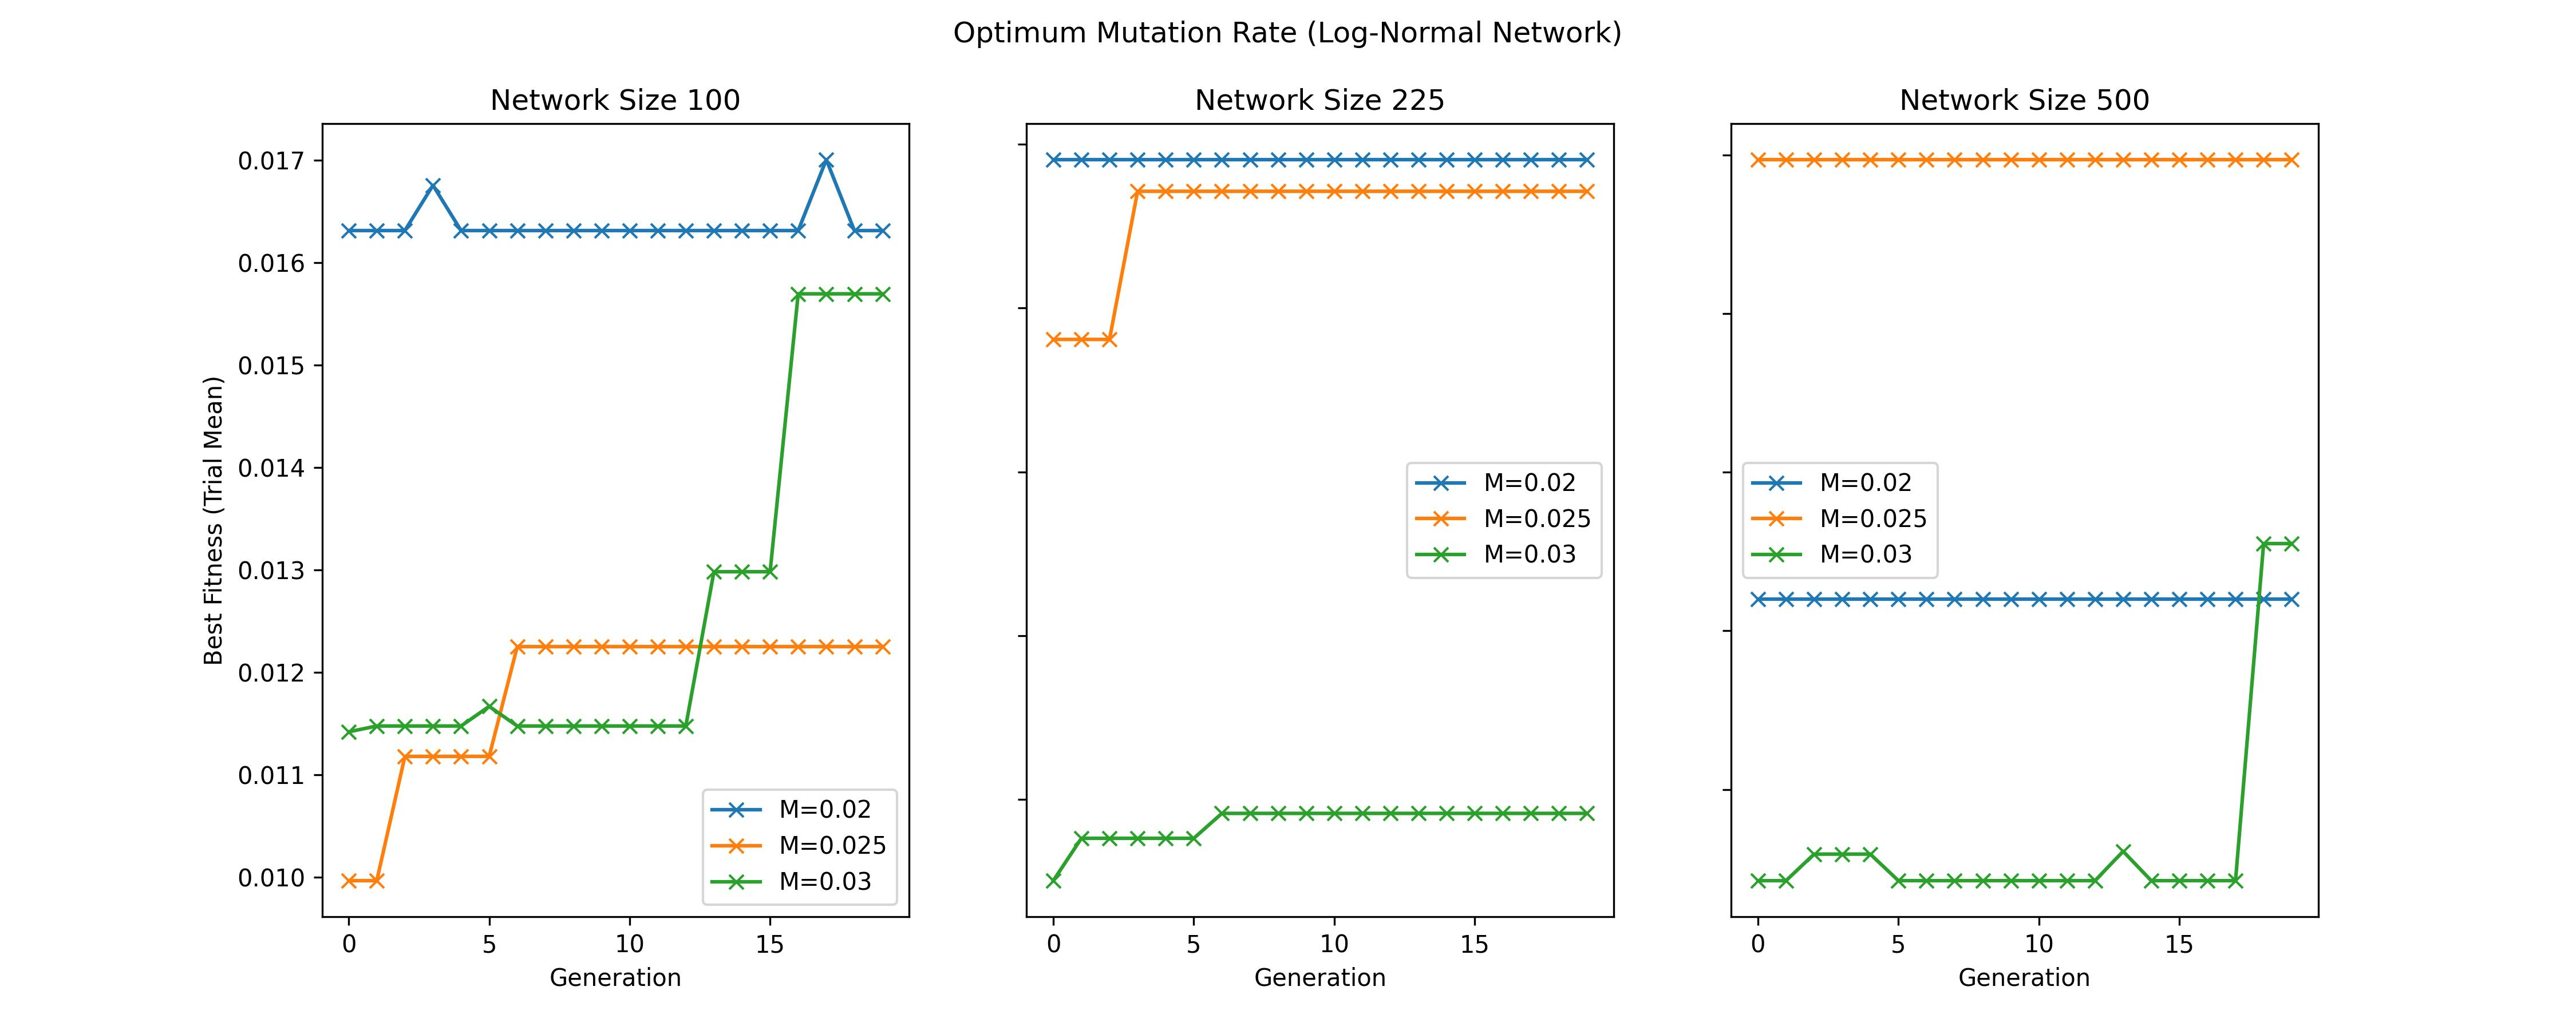
\includegraphics[width=\linewidth]{Figures/sims/mutation/optimum.jpg}
	\caption{BGF for a range of mutation rates in LN graphs. Mean of three trials. Results are variable. \emph{Produced in Python}}. 
	\label{fig:mutation_opt}
\end{figure*}

\begin{figure*}
	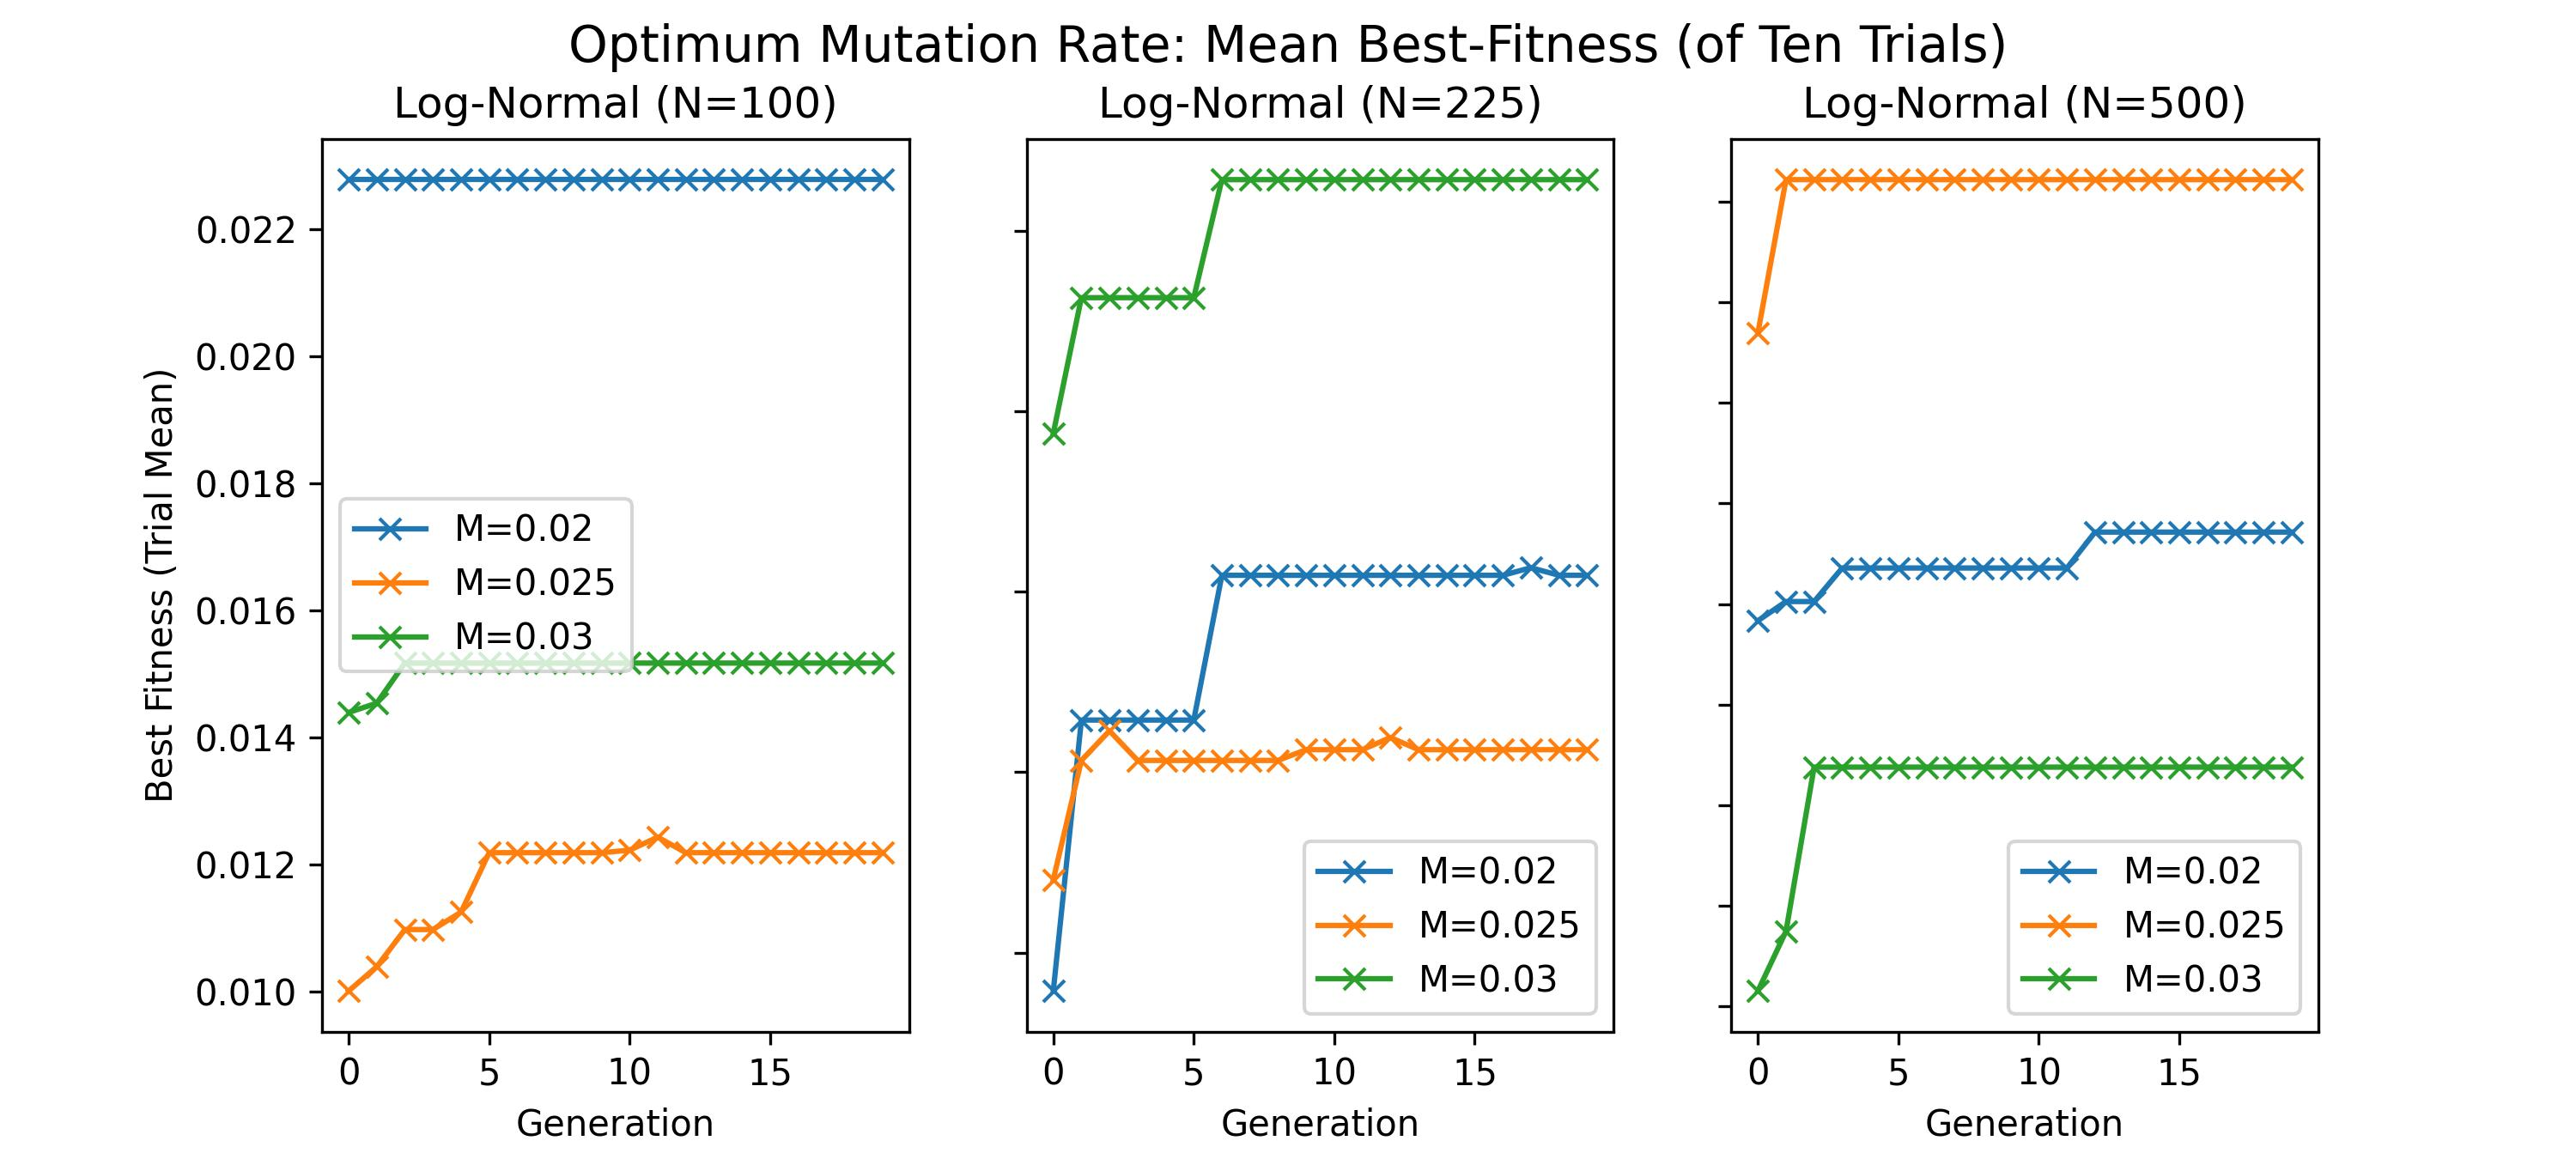
\includegraphics[width=\linewidth]{Figures/sims/mutation/optimum_ten.jpg}
	\caption{BGF for a range of mutation rates in LN graphs of sizes \(100, 225, 500\). Mean of ten trails.  \emph{Produced in Python}}. 
	\label{fig:mutation_opt_2}
\end{figure*}

The results are variable. The face value of the results would indicate that a mutation rate of \(0.02\) is optimal for network size \(100\); and \(0.025\) is optimal for network size \(500\). However, the results for size \(225\) are conflicting. Further to this, a test was conducted to record the mean solution (path converged to at threshold) fitness for several GA trials against a range of mutation rates: Figure \ref{fig:mutation_v_fitness}. This simulation indicates that on average mutation rate \(0.025\) converges to a better solution. 

\begin{figure}[H]
	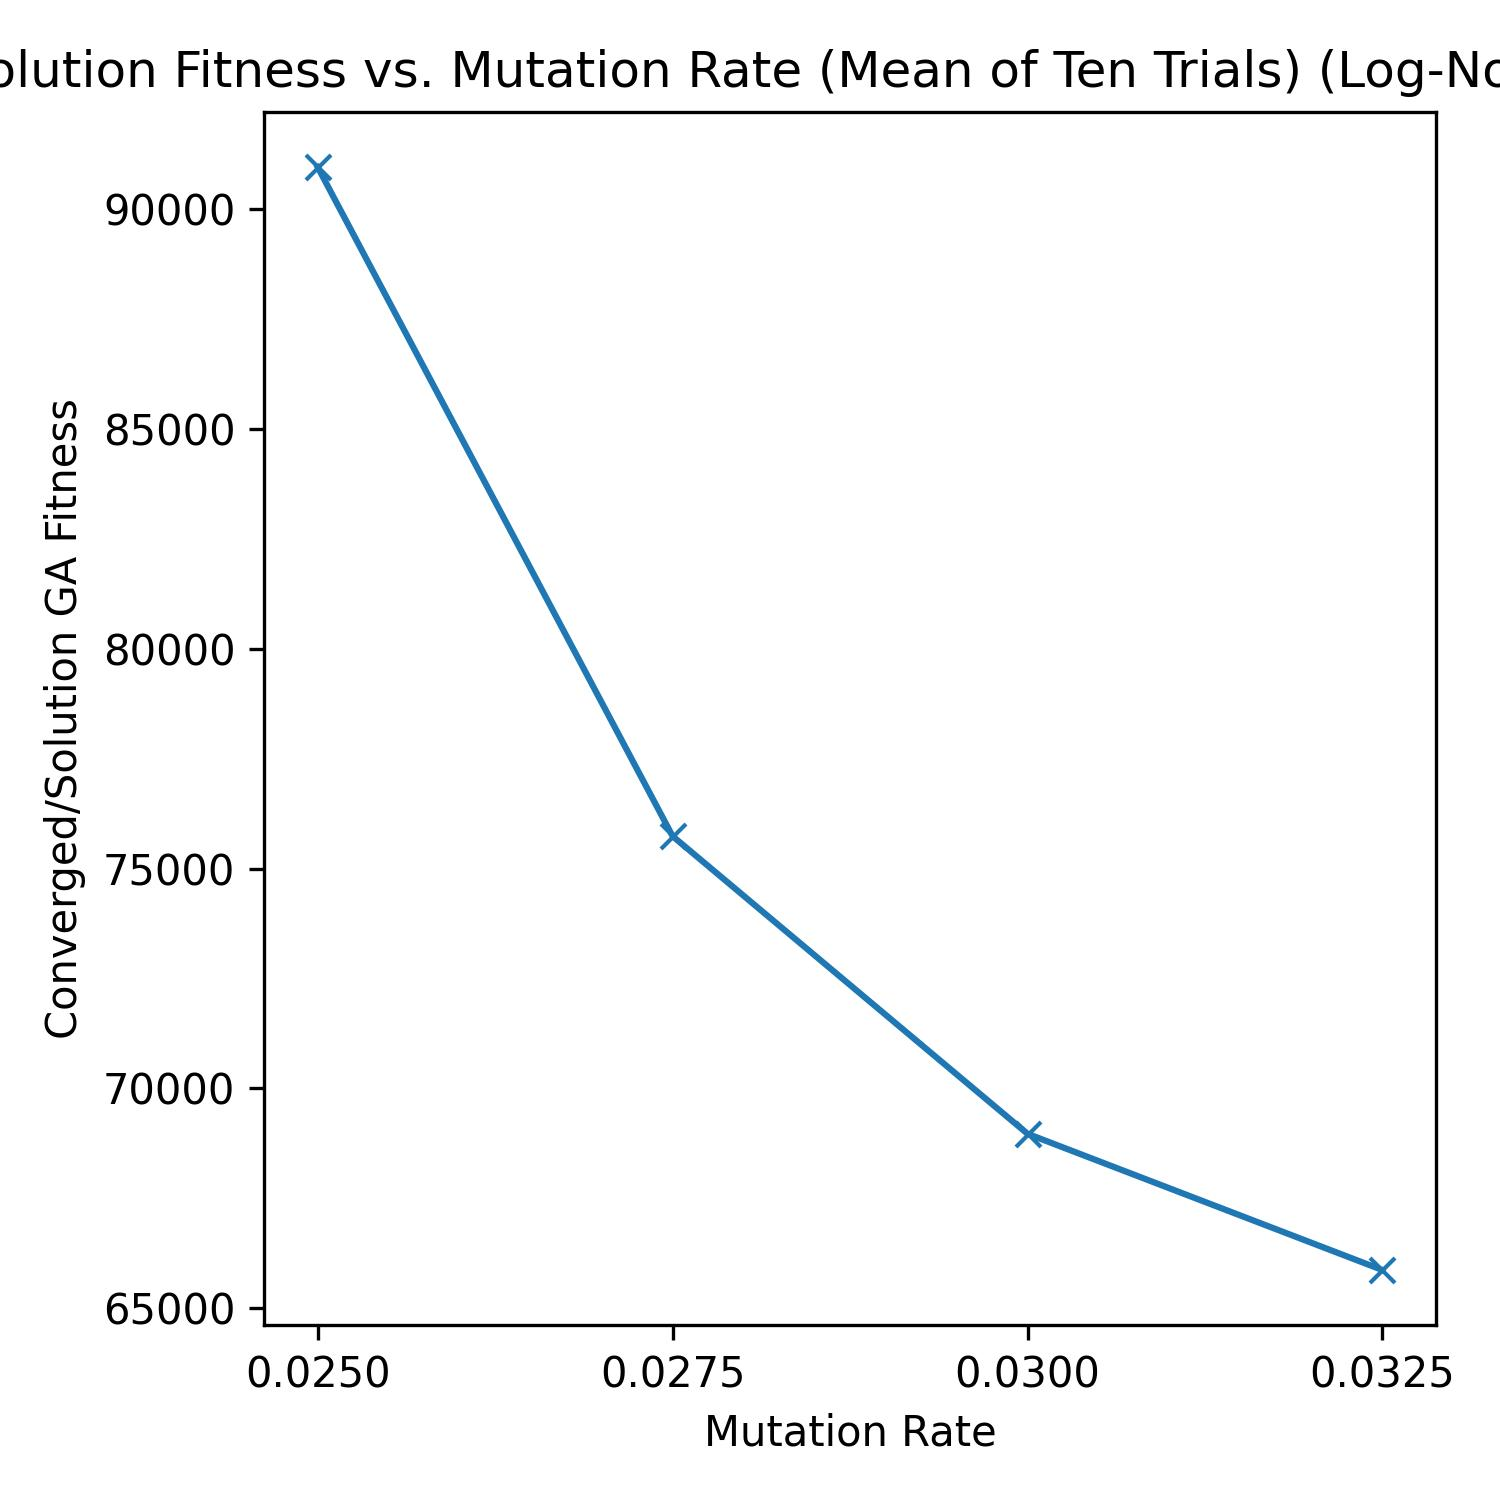
\includegraphics[width=\linewidth]{Figures/sims/mutation/mutation_v_fitness.jpg}
	\caption{Solution fitness of Specialised GA for a range of mutation rates in LN 500 graphs. Mean of ten trails.  \emph{Produced in Python}}. 
	\label{fig:mutation_v_fitness}
\end{figure}

\subsection{GA Static Performance}

This section presents the results of simulations run over each static topology considered to ascertain the performance of each variation of the Specialised GA: Standard (no immigrants); RIGA; EIGA; HIGA. The random topologies are initiated with the following parameters: 
\begin{enumerate}
	\item Graph sizes: [100, 225, 500] 
	\item Watts-Strogtaz: n = [sizes], k = 4, p = 0.25 
	\item Barabsi-Albert: n = [sizes], m = 3 
	\item Log-Normal: n = [sizes], degree = [500, 1125, 2500] 
\end{enumerate}

Simulations 1 and 2 are computed with population size \(120\) and fraction of population to be replaced with immigrants \(ri = 0.15\), \(ei = 0.1\). The GA is run for \(30\) iterations. \\

\subsubsection{Simulation 1} For each trial, a new graph for each static topology is generated and each variation of the GA is run for this same graph. In this simulation, the mean of results for multiple trials is not taken. The results plotted are the raw BGF of one run for each GA-Topology combination: Figure \ref{fig:static_1}.

\begin{figure*}
	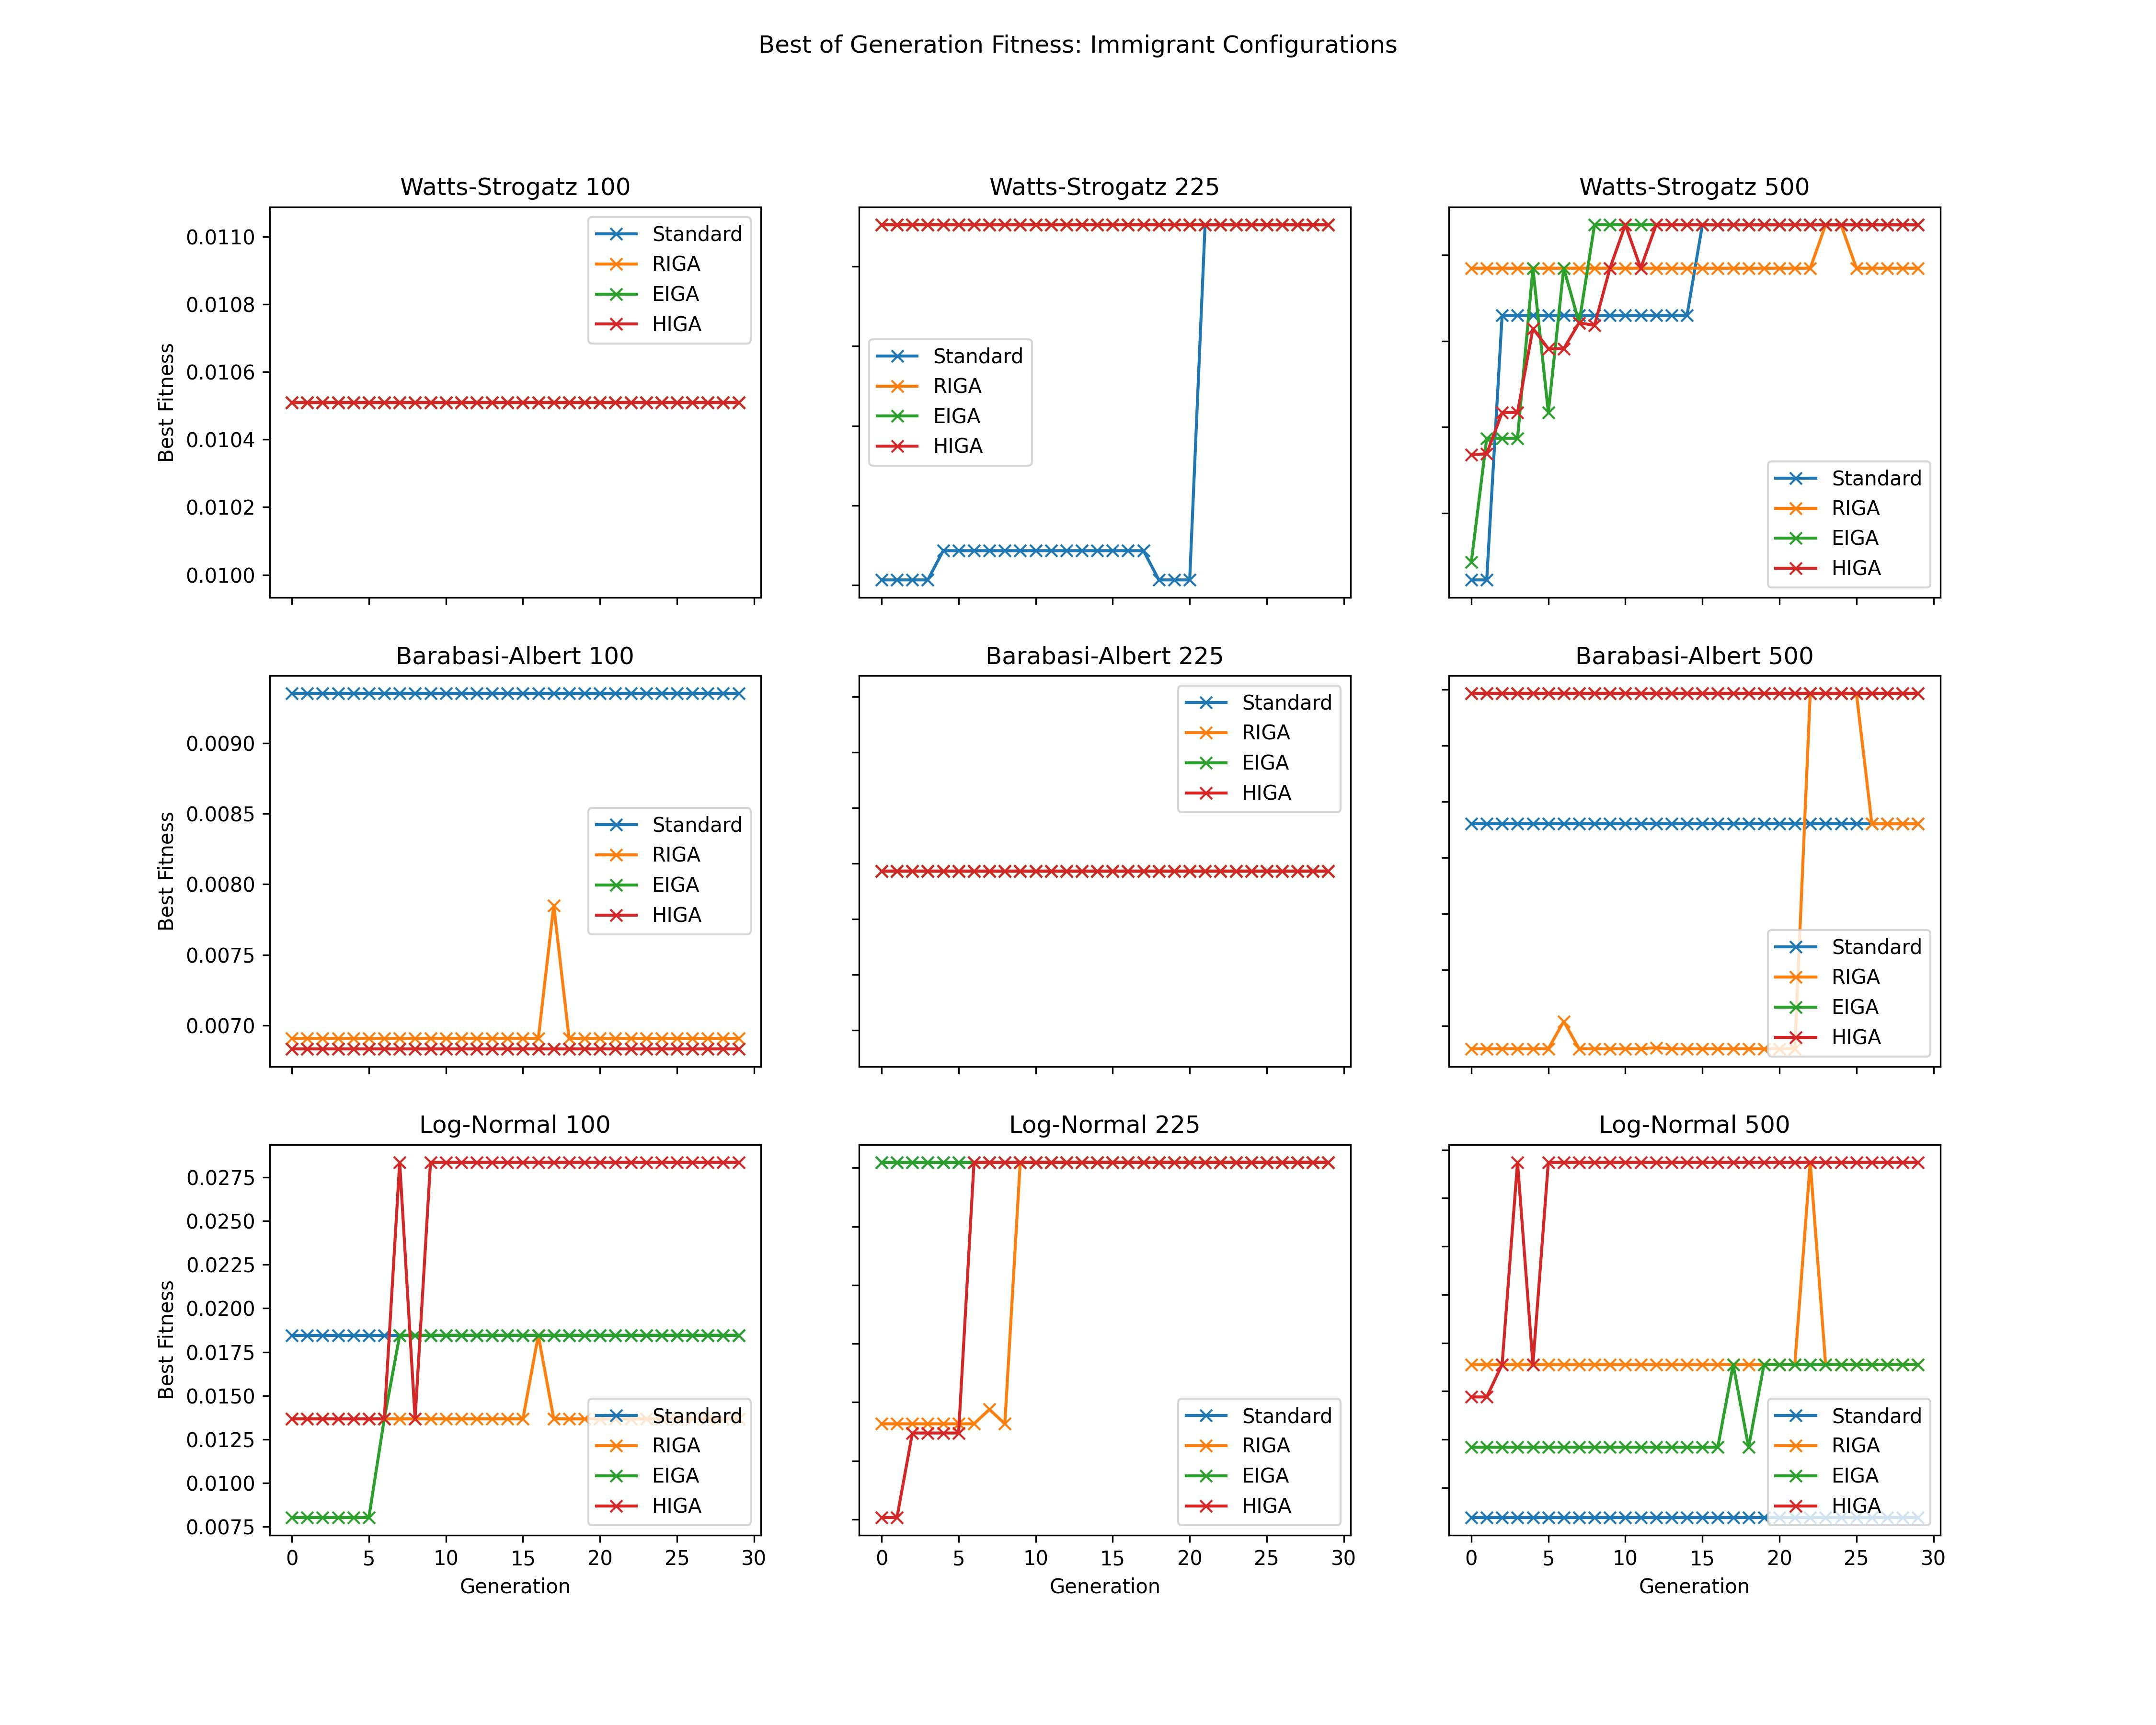
\includegraphics[width=\linewidth]{Figures/sims/static/experiment_1.jpg}
	\caption{BGF of each GA for static topologies.  \emph{Produced in Python}}. 
	\label{fig:static_1}
\end{figure*}

\subsubsection{Simulation 2} The results of \textbf{Simulation 1} are difficult to interperet as it is not clear at what points any of the GA's are performing optimally. The simulation is repeated here for new random topologies, where the target optimal fitness of the true shortest path for each graph and source/destination vertex pair is plotted as a black horizontal line on each graph to be compared with the BGF. Figure \ref{fig:static_2}. 

\begin{figure*}
	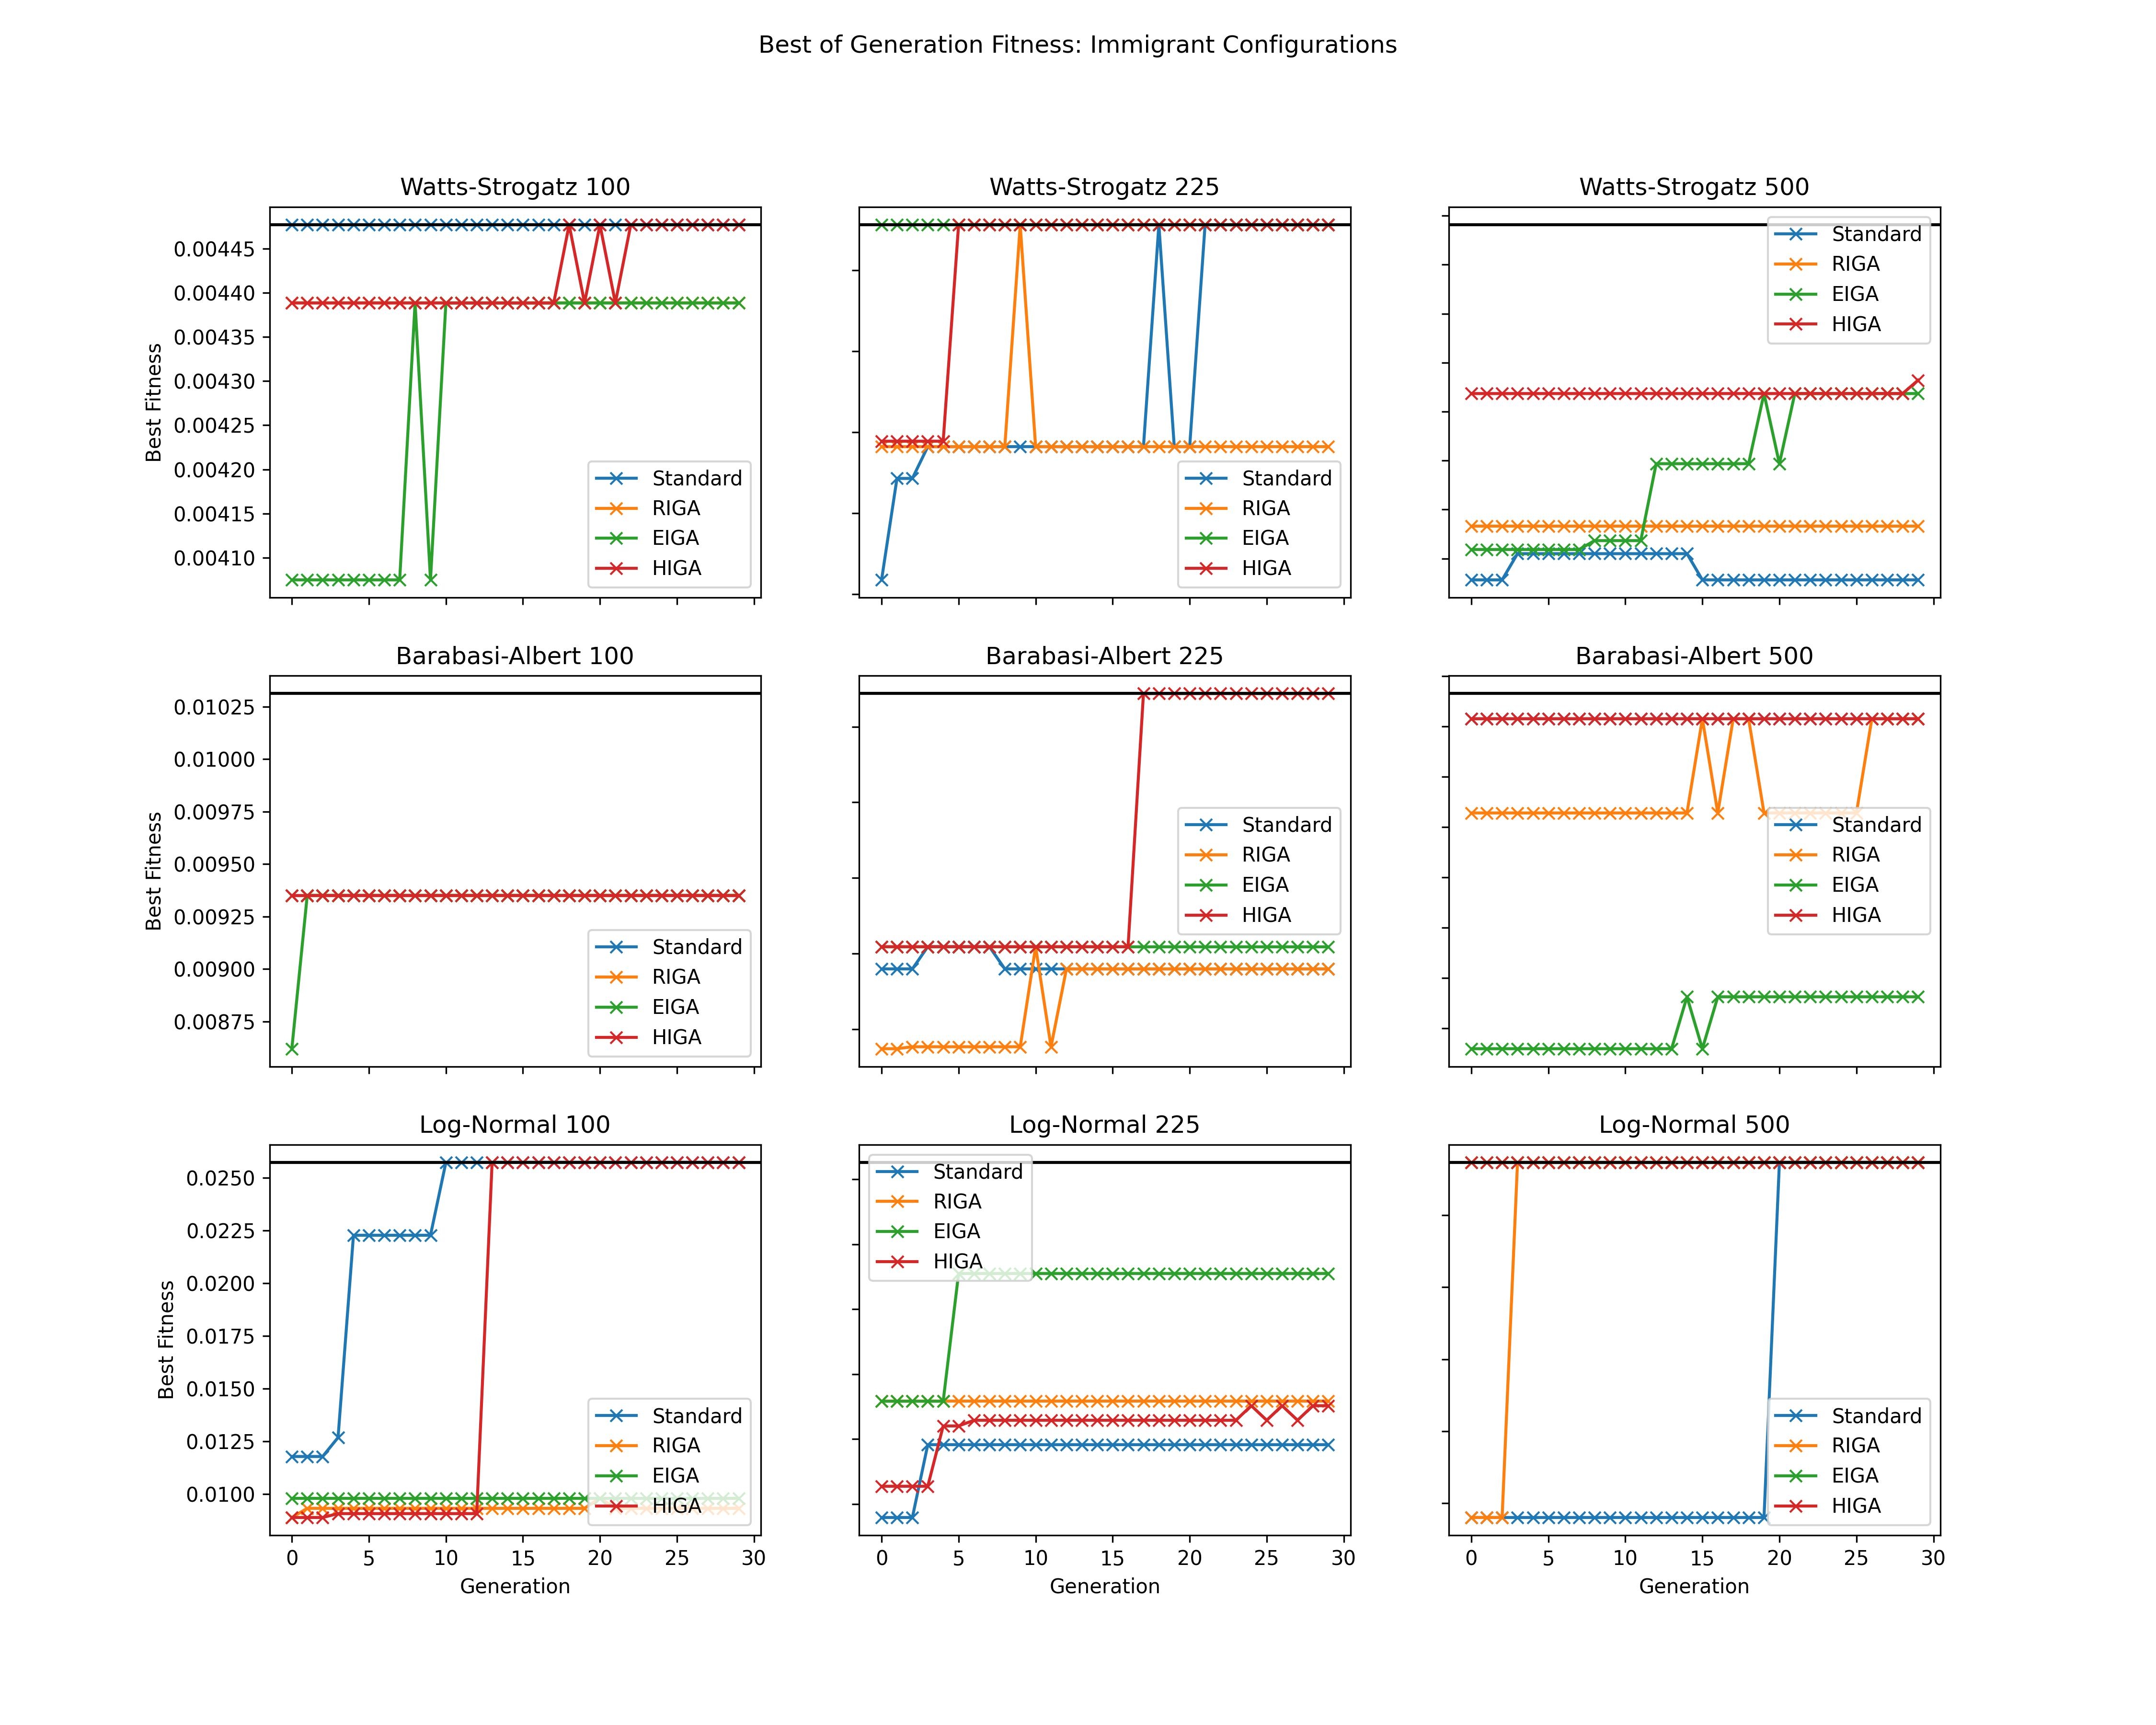
\includegraphics[width=\linewidth]{Figures/sims/static/experiment_2.jpg}
	\caption{BGF of each GA for static topologies with target optimal fitness of true shortest path (Horizontal black line) computed with Dijkstra's. \emph{Produced in Python}}. 
	\label{fig:static_2}
\end{figure*}

\subsubsection{Simulation 3} The simulation is repeated for the optimum population size and random immigrants factor \(ri = 0.1\) suggested by Yang \& Wang \cite{yang:10}: Figure \ref{fig:static_3}. 

\begin{figure*}
	\includegraphics[width=\linewidth]{Figures/sims/static/experiment_3.jpg}
	\caption{BGF of each GA for static topologies with target optimal fitness of true shortest path (Horizontal black line) computed with Dijkstra's. Population size 100; RI = 0.1, EI = 0.1 \emph{Produced in Python}}. 
	\label{fig:static_3}
\end{figure*}

\subsubsection{Simulation 4} Having identified the tendency of the RIGA; EIGA; HIGA to converge to the true optimal solution, with some exceptions where the algorithm falls into local optima, the final simulation over a static topology aims to provide a meaningful relative comparison of the training pattern and maximum fitness of each variation of the Specialised GA. Ten trials of the previous simulation structure are run and the average of corresponding results taken. For each trial, a new set of topologies are generated and the GA instances are run on the same generated topology for each subplot such that the BGF results are comparable.\\

\begin{figure*}
	\includegraphics[width=\linewidth]{Figures/sims/static/experiment_4.jpg}
	\caption{Mean BGF for each GA for the static topologies of ten trials. Population size 100; RI = 0.1, EI = 0.1. Results indicate that HIGA performs best overall whilst elitist methods are optimal for BA / Scale-Free networks. \emph{Produced in Python}}. 
	\label{fig:static_4}
\end{figure*}

Figure \ref{fig:static_4} plots the mean BGF for each topology. In summary, the results indicate that the HIGA performs best on average across all topologies and in particular for Log-Normal networks. For Watts-Strogatz networks both EIGA and the standard GA show simillar average performance to HIGA whilst RIGA shows consistently worse performance on average for the same graphs. Results with Barabasi-Albert networks are more variable. \\

This paper interprets that Barabasi-Albert networks are best solved with HIGA or EIGA, which show simillar performance. For BA networks, the RIGA and standard models show simillar performance. This indicates that routing in BA scale-free networks benefits from elitism more so than increased solution diversity. Other elitist methods of improving GA performance for DOPs may be investigated further for scale-free networks. \\

However, this paper woud note that results over static networks may be biased towards elitist solutions as compared with DSPRP simulations where diversity may be more valuable. From this perspective, it is interesting that HIGA outperforms EIGA. \\ 

\subsection{Dynamics: Change Probability Parameter} 

The first dynamic simulation takes HIGA as a representative and investigates the generational (BGF) performance for each topology under different probability parameters \(Pr_{dyn}\) to effect a change upon each component. Figure \ref{fig:prob_dyn} depicts the results, which are raw from one trial and are not averaged across multiple experiments as with some results presented in this paper. This paper interprets that HIGA shows the desired convergence behaviour overall, whereby the search moves towards higher fitness solution and shows peaks and troughs of fitness as in Yang \& Wang \cite{yang:10} which can be interpreted as the BGF being reset by topological changes, before the GA recovers fitness and converges again to a good solution without restarting the population. \\

In terms of relative performance between probability parameters, it is evident that at \(Pr_{dyn} = 0.01\) there is more stability and the GA remains converged for longer periods of time before the BGF is effected by a change. For higher values, the GA fitness resets more frequently however it appears to recover reliably for \(Pr_{dyn} = 0.05\) and ahcieve high fitness solutions. Hence, it is concluded that \(Pr_{dyn} = 0.05\) effects frequent change upon the shortest paths in each topology but that this can be tolerated by the GA. The probability paramter \(Pr_{dyn} = 0.05\) is used in the subsequent simulations.  

\begin{figure*}
	\includegraphics[width=\linewidth]{Figures/sims/dynamic/prob_dyn.jpg}
	\caption{Dynamic simulations for HIGA over each topology with varied probability parameters  \(Pr_{dyn} = 0.01, 0.025, 0.05\).\emph{Produced in Python}}. 
	\label{fig:prob_dyn}
\end{figure*}

\subsection{Dynamic Simulations} 

For each topology series, and with each model of stochastic topological dynamics proposed, simulations have been run taking the mean of ten trials BGF for each GA variation: Specialised/Standard GA (no immigrants); RIGA; EIGA; HIGA. The results indicate that, even in a dynamic environment with changes affecting the target shortest path several times per run as verified with Dijkstra's shortest path algorithm at each generation, the GA can recover and re-converge to the new optimal solution without restarting the population. Further investigation is required, but this paper interprets the results as showing the HIGA has the best overall performance. \\ 

\subsubsection{Simulation 1} In this simulation topological dynamics of the weight set are simulated over each static topology, with probability parameter \(Pr_{dyn} = 0.05\) which has been demonstrated to effect the shortest paths. Each variation of the GA is run in each of the simulated network environments ten times and the mean of BGF is taken. The population size is set at \(100\) and mutation rate at \(0.03\). The Random/Elitist immigrants fraction is set at \(0.1, 0.1\) for HIGA and \(0.2\) for EIGA and RIGA. Figure \ref{fig:dynamic_1} \ref{fig:dynamic_2}. 

\begin{figure*}
	\includegraphics[width=\linewidth]{Figures/sims/dynamic/series_a_weight.jpg}
	\caption{Dynamic simulations for the weight-set over each topology. \(Pr_{dyn} = 0.05\).\emph{Produced in Python}}. 
	\label{fig:dynamic_1}
\end{figure*}

\begin{figure*}
	\includegraphics[width=\linewidth]{Figures/sims/dynamic/series_a_weight_2.jpg}
	\caption{\#2 Dynamic simulations for the weight-set over each topology. \(Pr_{dyn} = 0.05\).\emph{Produced in Python}}. 
	\label{fig:dynamic_2}
\end{figure*}

\subsubsection{Simulation 2} The same structure of simulation as in \textbf{Simulation 1} is run with topological dynamics of the edge set. Figure \ref{fig:dynamic_3} \ref{fig:dynamic_4}. 

\begin{figure*}
	\includegraphics[width=\linewidth]{Figures/sims/dynamic/series_b_edge.jpg}
	\caption{Dynamic simulations for the edge-set over each topology. \(Pr_{dyn} = 0.05\).\emph{Produced in Python}}. 
	\label{fig:dynamic_3}
\end{figure*}

\begin{figure*}
	\includegraphics[width=\linewidth]{Figures/sims/dynamic/series_b_edge_2.jpg}
	\caption{\#2 Dynamic simulations for the edge-set over each topology. \(Pr_{dyn} = 0.05\).\emph{Produced in Python}}. 
	\label{fig:dynamic_4}
\end{figure*}

\subsubsection{Simulation 3} The same structure of simulation as in \textbf{Simulation 1} is run with topological dynamics of the node set. Figure \ref{fig:dynamic_5} \ref{fig:dynamic_6}.

 \begin{figure*}
	\includegraphics[width=\linewidth]{Figures/sims/dynamic/series_c_node.jpg}
	\caption{Dynamic simulations for the node-set over each topology. \(Pr_{dyn} = 0.05\).\emph{Produced in Python}}. 
	\label{fig:dynamic_5}
\end{figure*}

\begin{figure*}
	\includegraphics[width=\linewidth]{Figures/sims/dynamic/series_c_node_2.jpg}
	\caption{\#2 Dynamic simulations for the node-set over each topology. \(Pr_{dyn} = 0.05\).\emph{Produced in Python}}. 
	\label{fig:dynamic_6}
\end{figure*}

\subsubsection{Simulation 4} The previous dynamic simulations \textbf{1-3} have a limitation. For each subplot specifying the static topology to which dynamics are applied, a new instance of the topology is generated not only for every trial but for each GA variation. The consequence of this is that the BGF data for each GA variation, for each run, is computed over a distinct graph such that the results are not directly comparable. Furthermore, dynamics are applied independently to each separate graph. \\

In order for the resutls reported for each GA variation to be synchronised and comprabale at each generation, the GA variations should be solving the same for the same source and destination vertices over the same graph in each trial. Then, this simulation design carries the additional benefit that dynamics need only be applied to the single graph for each topology, for each run and Dijkstra's algorithm can be used to calculated the true shortest path at each generation for objective comparison with the BGF. \\

These improved simulations are referred to as being \emph{synchronised}. Figure \ref{fig:dynamic_7} presents the results of the synchronsied simulation for topological dynamics of the edge weights. Figure \ref{fig:dynamic_8} presents the results of the synchronised simulation for topological dynamics of the edge set. Figure \ref{fig:dynamic_9} presents the results of the synchronised simulation for topological dynamics of the node set. For each simulation, the target optimal fitness of the true shortest path at each generation is marked in the dashed black line. \\

% Figures 
 \begin{figure*}
	\includegraphics[width=\linewidth]{Figures/sims/dynamic/series_a_weight_sync.jpg}
	\caption{Synchronised dynamic simulations for the weight-set over each topology. \(Pr_{dyn} = 0.05\).\emph{Produced in Python}}. 
	\label{fig:dynamic_7}
\end{figure*}

 \begin{figure*}
	\includegraphics[width=\linewidth]{Figures/sims/dynamic/series_b_edge_sync.jpg}
	\caption{Synchronised dynamic simulations for the edge-set over each topology. \(Pr_{dyn} = 0.05\).\emph{Produced in Python}}. 
	\label{fig:dynamic_8}
\end{figure*}

 \begin{figure*}
	\includegraphics[width=\linewidth]{Figures/sims/dynamic/series_c_node_sync.jpg}
	\caption{Synchronised dynamic simulations for the node-set over each topology. \(Pr_{dyn} = 0.05\).\emph{Produced in Python}}. 
	\label{fig:dynamic_9}
\end{figure*}

\subsubsection{Interpretation of Results} The learning pattern as depicted by the BGF values is encouraging: For static topologies where the target maximum fitness is stable the Specialised GA variants achieve optimal or near optimal fitness in most cases (Figure \ref{fig:static_2}; Figure \ref{fig:static_3}). For dynamic topologies, the most interpretable results are offered by the synchronised simulations with target-fitness calculation: Figure \ref{fig:dynamic_7}, Figure \ref{fig:dynamic_8} and Figure \ref{fig:dynamic_9}. Performance is also promising for dynamic series. The pattern exhibited is that the generation fitness will decrease after a change in topology before recovering to near optimal fitness within a few generations, simply by continuing to evolve the existing population. In some plots, for instance in the synchronous dynamic simulation over Topology Series A: Dynamic Weight Set (Figure \ref{fig:dynamic_7}), examples of the desired GA performance can be seen, for instance in the WS models, where the BGF closely maps the target fitness with convergence to new global optima with one or two generations of a change and minimal deviation. Across all Topology Series are instances where the search becomes stuck at local optima, however, and methods to encourage more consistent convergence need to be investigated further. \\

The relative performance of the Specialised GA variants and performance for different topology series is less clear. Interestingly, performance over the Log-Normal topologies generated appears to be consistently poor as compared with WS and BA models. However, this paper interprets that EIGA and HIGA deviate least from the target fitness for LN models and hence reccommend further investigations into the cause of poor performance and potential remedies, with a focus on Elitist strategies. Barabsi-Albert models are solved well and appear to be best solved with EIGA or HIGA elitist strategies. Watts-Strogatz models are solved most reliably and show best performance with RIGA and HIGA suggesting that diversity strategies are useful for routing in small worlds. \\

With respect to the topological dynamics defined, all three methods appear to be handled well. For a 5\% chance to effect a change upon each component, Topology Series C (Figure \ref{fig:dynamics_9}, node set dynamics) appeared the most turbulent causing frequent sharp changes in BGF. However, the HIGA variant of the Specialised GA performed well on average with the exception of in LN models where convergence to the (near) optimal fitness was less frequent. Both Topology Series A \& B, weight and edge set dynamics, appeared to be solved reliably where better marginally better performance may be interpreted for T. Series A (Figure \ref{fig:dynamics_8}, \ref{fig:dynamics_8}. Topology Series B was solved particularly well for WS, BA and small \(n = 100\) LN models: Figure \ref{fig:dynamic_8}. 

\subsection{Best of Generation Accuracy} 

The Best of Generation Fitness (BGF) provides one lense within which to view the performance of the GA.  Simulations taking the mean of ten trials have been conducted for each topology and dynamic, recording the BGF of each run. These simulations offer a partial view, however the BGF metric does not well represent the error between the GA fitness and true optimum solution at each generation. Then, a new measure of algorithm performance is introduced: Best of Generation Accuracy (BGA) Eq. \ref{eq:bga}. 

\begin{equation}
	bga_{i} = \frac{bgf_{i}}{target_{i}}
	\label{eq:bga}
\end{equation}

The BGA is calculated as the BGF divided by the target optimal fitness for that generation, calculated with Dijkstra's shortest path algorithm. Then, the BGA is a score in the range \([0, 1]\) where a score of \(1.0\) indicates the generation has achieved target maximal fitness. \\

Simulations have been conducted which calculated the mean BGA (mBGA) for each run, and the mean of the mBGA calculated over ten trials for each GA and topology have been recorded. \\

\subsubsection{Weight Set mBGA} 
\begin{center}
\begin{tabular}{||c c c c c||} 
 \hline
 \emph{Graph} & Standard & RIGA & EIGA & HIGA \\ [0.5ex] 
 \hline\hline
 WS & 0.766668 & 0.819361 & 0.748040 & 0.814541 \\ 
 \hline
 BA & 0.600757 & 0.603461 & 0.630320 & 0.623035 \\
 \hline
 LN & 0.472843 & 0.588114 & 0.574488 & 0.578455 \\
\end{tabular}
\end{center}

\subsubsection{Edge Set mBGA} 
\begin{center}
\begin{tabular}{||c c c c c||} 
 \hline
 \emph{Graph} & Standard & RIGA & EIGA & HIGA \\ [0.5ex] 
 \hline\hline
 WS & 0.240832 & 0.301248 & 0.312507 & 0.261252 \\ 
 \hline
 BA & 0.256440 & 0.245533 & 0.224812 & 0.286415\\
 \hline
 LN & 0.174980 & 0.106760 & 0.124692 & 0.128604  \\
\end{tabular}
\end{center}

\subsubsection{Node Set mBGA}

\begin{center}
\begin{tabular}{||c c c c c||} 
 \hline
 \emph{Graph} & Standard & RIGA & EIGA & HIGA \\ [0.5ex] 
 \hline\hline
 WS & 0.423773 & 0.424486 & 0.428482 & 0.390456 \\ 
 \hline
 BA & 0.331057 & 0.339533 & 0.375910 & 0.426892 \\
 \hline
 LN & 0.257281 & 0.273855 & 0.251358 & 0.185078 \\
\end{tabular}
\end{center}

These results indicate that on average the quality of solutions produced at each generation are poor. However, this may not neccessarily indicate that the overall performance of the GAs is very poor. In principle, the requirement of the GA in a dynamic environment is to achieve but not neccesarily to remain at a high fitness region of the search space. For most generations, the GA may reside in a low fitness region from which it moves towards a high fitness region. The GA may function well and converge to a high fitness solution, but spend the majority of generations in a low fitness region especially as a consequence of dynamic changes. The high fitness regions need only be achieved for a few generations for the solution to be returned and used; the mBGA metric may not fully reflect the successful search behaviour and convergence of the GA. \\

Considering the mBGA as a measure of relative performance only, this paper interprets that for the Edge Set Dynamics RIGA/HIGA perform best for Watts-Strogatz graphs; whilst HIGA outperforms for Barabasi-Albert graphs; interestingly, the no-immigrants standard Sepcialised GA outperforms for Log-Normal graphs even under edge dynamics. \\

For the Node Set Dynamics, it is observed again that elitism techniques produce better performance in Barabasi-Albert Scale Free networks as EIGA/HIGA outperform the standard and RIGA variations. For WS graphs simillar performance is seen for each variation excepting HIGA which underperforms. For LN graphs RIGA produces the best performance.\\

For Weight Set Dynamics, the RIGA, EIGA and HIGA outperform the standard Specialised GA with RIGA/HIGA performing best for Watts-Strogatz graphs suggesting that diversity should be emphasised over elitism for Small-Worlds; HIGA and EIGA outperform again for Barabasi-Albert graphs and LN graphs are simillarly solved with RIGA, EIGA and HIGA.  \\

From this, this paper conlcudes that RIGA; EIGA and HIGA are similarly additionally  effective in the dynamic environments constructed for moderate chagne probably \(Pr_{dyn} = 0.05\) under which condition change is expected at every generation, however the target shortest path is no neccessarily affected. Elitism strategies are likely more effective in general for Scale-Free networks whilst diversity can be emphasised to produced better solutions in Small-Worlds. \\ 

Then, a second metric is devised to compare the relative performance of the GA variations where emphasis is placed upon convergence to the optimal solutions. For one hundred generations, the number of generations achieving a BGA of \(1.0\) is recorded and used as a metric of search performance. 

\subsubsection{Edge Set Mean Generations at Target Fitness (/60 Generations)}
\begin{center}
\begin{tabular}{||c c c c c||} 
 \hline
 \emph{Graph} & Standard & RIGA & EIGA & HIGA \\ [0.5ex] 
 \hline\hline
 WS & 3.1 & 4.2 & 4.8 & 2.9 \\ 
 \hline
 BA & 0.9 & 1.5 & 2.1 & 4.5 \\
 \hline
 LN & 0.7 & 0.0 & 0.1 & 0.1 \\
\end{tabular}
\end{center}

\subsubsection{Weight Set Mean Generations at Target Fitness (/60 Generations)} 

\begin{center}
\begin{tabular}{||c c c c c||} 
 \hline
 \emph{Graph} & Standard & RIGA & EIGA & HIGA \\ [0.5ex] 
 \hline\hline
 WS & 8.1 & 9.6 & 6.8 & 11.2 \\ 
 \hline
 BA & 4.1 & 3.0 & 4.5 & 3.5 \\
 \hline
 LN & 9.0 & 12.1 & 11.8 & 11.7 \\
\end{tabular}
\end{center}

\subsubsection{Node Set Mean Generations at Target Fitness (/60 Generations)}

\begin{center}
\begin{tabular}{||c c c c c||} 
 \hline
 \emph{Graph} & Standard & RIGA & EIGA & HIGA \\ [0.5ex] 
 \hline\hline
 WS & 5.2 & 6.0 & 5.7 & 5.8 \\ 
 \hline
 BA & 8.8 & 8.5 & 11.9 & 12.8 \\
 \hline
 LN & 2.2 & 3.0 & 3.8 & 0.1 \\
\end{tabular}
\end{center}

These results interestingly indicate that the different topological dynamics have a distinct effect upon GA performance across variations and topologies, even for the same probability parameter. Results for the weight set dynamics are broadly higher indicating more frequent convergence to the true optimum. Node set dynamics generally produce less frequent convergence to the optimum although better performance is ahcieved for BA scale-free graphs. Edge set dynamics produce the poorest performance by a significant margin. This is possibly because the edge rewiring process causes each topology to devolve into an ER uniform random-graph. \\

Overall, RIGA and HIGA perform better in WS graphs excepting in the case of edge set dynamics where EIGA is more effective. BA graphs are best solved with EIGA, HIGA with little variability. LN graphs benefit from both EIGA and HIGA except in the case of Edge-Set dynamics where convergence approaches zero. 


%------------------------------------------------
\section{Conclusion and Future Work} 

This paper has investigated the DSPRP in random networks with Small-World and Scale-Free properties and Log-Normal degree distributions which are believed overall to be empirically ubiquitous and relevant to communications networks. Small-World and Scale-Free properties have been identified in computer networks, and have further been investigated as a means to improve the routing performance of wireless MANETs and IoT networks \cite{sohn:17} \cite{dong:15}. Building upon existing investigations into the performance of Genetic Algorithms for the DSPRP \cite{yang:10} \cite{kumar:10}, this paper devised three models of topological dynamics effecting each separate aspect of the network architecture. Variations of a Specialised GA for the SSSP were written, based on the work of \cite{yang:10}, employing Random, Elitism and Hybrid Immigrant schemes in order to improve performance in dynamic topologies. \\

In simulations, performance of the developed solutions was somewhat variable but promising. The RIGA, EIGA and HIGA GA's proposed have been demonstrated to be able to consistently converge to the optimal or near optimal shortest path in moderately dynamic environments in most cases: Figure \ref{fig:dynamic_7}, \ref{fig:dynamic_8}, \ref{fig:dynamic_9}. In terms of contributions to the overall understanding of the DSPRP, the results of this paper indicate that routing in dyamic Scale-Free networks benefits most from elistist strategies such as the EIGA. Conversely, Small-World topologies may be better solved with strategies emphasising diversity such as RIGA. Densely connected Log-Normal topologies, as they were generated in this paper where the number of edges is ~5x the number of nodes, present a unique challenge with repsect to the DPSPR and convergence to the true optimum was observed to be relatiely rare. \\ 

Further work is required with respect to methods of simulating realistic topological dynamics. For instance, the method of simulating dynamics of the edge set in this paper tended to effect the statistical properties such as the average pathelength, by incrementally randomising the network, of the initial topologies and this may have resulted in biased simulations. Furthermore, results for the Edge Set dynamics given in the form of the mBGA and average number of generations with true optimal fitness suggested poor performance in lieu of the promising picture painted by the visual simulations. Both methods of assessing the reliability of the GAs are flawed; new metrics of evaluation for DSPRP performance are required. \\ 

The path generation method used in this paper, also used in other works \cite{yang:10} \cite{kumar:10} \cite{yussof:09}, is expensive and scales poorly with the size of the network. Whilst population generation only needs to be commited once before the GA can run, the setting in which networks may need to restart may pose a practical problem considering that population generation for graph of size \(n \geq 500\) took over 100 seconds to compute on an industry standard commercial personal computer. The method of selection used, Stochastic Unviersal Sampling, is also fairly inefficient and future work could investigate  alternatives such as Tournament Selection. \\

There are many interesting cases for future works to build upon this research and propose new and more interesting solutions. For example, \cite{yussof:09} investigates the efficacy of various parallel GA implemnetations for the static SSSP problem that may be deployed over a network of compute nodes which may each maintain and evolve a separate small population. This paper recommends that an intersting and relevant future work would be to combine the DSPRP solution proposed with Yussof et al's parallel archiecture to create parallel solution the DSPRP which may be suited to deployment on real wireless networks, especially where the computing resources at each node are limited. \\


%----------------------------------------------------------------------------------------
%	 REFERENCES
%----------------------------------------------------------------------------------------

\printbibliography % Output the bibliography

%----------------------------------------------------------------------------------------

\end{document}
